\documentclass{article}
% \usepackage[preprint]{neurips_2026}
\usepackage[preprint]{neurips_2026}
\usepackage[T1]{fontenc}
\usepackage[utf8]{inputenc}
\usepackage{microtype}
\microtypesetup{expansion=false}
%\usepackage{inconsolata}
\usepackage[table]{xcolor}
\usepackage{graphicx}
\usepackage{booktabs}
\usepackage{amsmath}
\usepackage{amssymb}
\usepackage[normalem]{ulem}
\usepackage{float}
\usepackage{tabularx}
\usepackage[breakable, skins]{tcolorbox}
\usepackage{makecell}
\usepackage{fvextra}
\usepackage{multirow}
\usepackage{subcaption}
\usepackage{dsfont}
\usepackage{threeparttable}
\usepackage{longtable}
\usepackage{siunitx}
%\usepackage{tikz}
%\usepackage{etoc}
\usepackage{hyperref}

\setcitestyle{citesep={;}}

\makeatletter
\newcommand{\appendixsection}[1]{%
  \section{#1}%
  \addcontentsline{apc}{section}{\protect\numberline{\thesection}#1}%
}

\newcommand{\appendixcontents}{%
  \section*{Appendix Contents}%
  %\begin{NoHyper}
  \@starttoc{apc}%
  %\end{NoHyper}
}
\makeatother

\newcolumntype{Y}{>{\centering\arraybackslash}X}

\newtcolorbox{promptbox}[1][]{
    breakable,
    enhanced,
    colback=gray!5,
    colframe=gray!60!black,
    boxrule=0.5pt,
    arc=2pt,
    left=6pt, right=6pt, top=6pt, bottom=6pt,
    fonttitle=\bfseries\sffamily\small,
    coltitle=black,
    colbacktitle=gray!15,
    attach boxed title to top left={yshift=-2mm, xshift=3mm},
    boxed title style={boxrule=0pt, colframe=gray!5, arc=2pt},
    title={#1},
    fontupper=\ttfamily\footnotesize,
}


% Primary colours
% =========================
% Green — correct / medical
% =========================
\definecolor{GreenDark}{HTML}{328132}
\definecolor{GreenMid}{HTML}{61CA53}
\definecolor{GreenLight}{HTML}{DCF5DC}

% =========================
% Orange — error / hallucination
% =========================
\definecolor{OrangeDark}{HTML}{D98A45}
\definecolor{OrangeMid}{HTML}{F1C38F}
\definecolor{OrangeLight}{HTML}{FBF1E6}

% =========================
% Purple —  secondary
% =========================
\definecolor{PurpleDark}{HTML}{75639B}
\definecolor{PurpleMid}{HTML}{B7A9D6}
\definecolor{PurpleLight}{HTML}{EEEAF5}



\definecolor{MedicalGreen}{HTML}{61CA53}
\definecolor{AmethystSmoke}{HTML}{B7A9D6}
\definecolor{ClinicalGrey}{HTML}{B0B0B0}
\definecolor{IcyBlue}{HTML}{CFE6FA}
\definecolor{SoftRose}{HTML}{D9A3B3}
\definecolor{darkgreen}{RGB}{50,129,50}
\definecolor{lightgreen}{RGB}{220,245,220}
\definecolor{lightgray}{RGB}{240,240,240}

% TODO commands 
\definecolor{JackGreen}{HTML}{228B22}
\definecolor{LilyPurple}{HTML}{8E44AD}
\definecolor{GriffinGrey}{HTML}{61CA53}
\definecolor{WilliamBlue}{HTML}{2471A3}
\definecolor{FabioRose}{HTML}{C44569}

\newcommand{\jack}[1]{\textcolor{JackGreen}{\textbf{[Jack: #1]}}}

\newcommand{\lily}[1]{\textcolor{LilyPurple}{\textbf{[Lily: #1]}}}

\newcommand{\griffin}[1]{\textcolor{GriffinGrey}{\textbf{[Griffin: #1]}}}

\newcommand{\william}[1]{\textcolor{WilliamBlue}{\textbf{[William: #1]}}}

\newcommand{\fabio}[1]{\textcolor{FabioRose}{\textbf{[Fabio: #1]}}}

\hypersetup{
  colorlinks=true,
  citecolor=darkgreen,
  linkcolor=darkgreen,
  urlcolor=darkgreen, 
  breaklinks=true
}

\interfootnotelinepenalty=10000

% When Rubrics Fail: 
% \title{When Rubrics Fail: Hallucinations Reveal Blind Spots in AI Medical Evaluation}
\title{When Rubrics Fail: Hallucinations Reveal Blind Spots in Medical AI Evaluation}
% \title{Rubric Blind Spots: How Medical Hallucinations Escape LLM Evaluation}
% \title{Rubric Blind Spots: Hallucinations in LLM Evaluation for Medical Applications}
% \title{When Rubrics Fail: Hallucinations Reveal Blind Spots in Medical AI Evaluation}
% \title{Hallucinations Reveal Rubric Blind Spots \\ in Medical LLM Evaluation}


\author{
Griffin Farrow$^{*}$ \\
University of Oxford
\And
Lily Sijia Li$^{*}$ \\
University of Oxford
\And
Jack Johnson$^{*}$ \\
University of Oxford
\AND
Tingyan Wang \\
University of Oxford
\And
Philip Torr \\
University of Oxford
\And
William Bolton \\
University of Oxford
\And
Fabio J. Fehr \\
University of Oxford
}

\begin{document}
\maketitle

%\begin{center}
%\vspace{-2.5em}
%\small
%\noindent\parbox{\textwidth}{\centering
%\href{https://www.youtube.com/watch?v=ovU4ESybz-U}{%
%    \raisebox{-0.45em}{
\includegraphics[height=1.6em]{figures/hg-logo.png}}\ Data
%}
%\quad\quad
%\href{https://www.youtube.com/watch?%    \raisebox{-0.2em}{
\includegraphics[height=1.2em]{figures/gh-logo.png}}\ Code
%}
%}
%\end{center}
\vspace{-1.5em}
\begin{abstract}
Hallucinations can undermine clinician trust in LLMs, making it important that evaluation methods capture clinically relevant errors. Rubric-based evaluation has become the leading approach for assessing LLMs in medicine, but it is unclear whether rubric scores reflect such errors. We first study this in a controlled setting using MedHallu, finding that more specific rubrics better distinguish correct from hallucinated responses. To test this systematically, we develop a taxonomy of medical hallucination types and a clinician-validated error-injection pipeline that creates matched correct and error-injected responses. Across HealthBench, HealthBench Professional, and LiveMedBench, our clinically relevant hallucinations are missed by rubrics, often leaving scores unchanged.  We find that rubrics are most effective when explicitly checking facts, and are less effective for additional or unexpected errors they do not anticipate. A preliminary retrieval-based factuality check recovers some of the rubric-blind errors, suggesting a complementary approach. These findings reveal systematic blind spots in current medical evaluation of LLMs and suggest that rubric scores alone are insufficient to establish clinical reliability, potentially undermining clinician trust and confidence in clinical deployment.
% Hallucinations can undermine clinician trust in medical LLMs, making it important that evaluation methods capture clinically important errors. Rubric-based evaluation has become a leading approach for assessing LLMs, but it is unclear whether rubric scores reflect such errors. We first study this in a controlled setting using MedHallu, finding that more specific rubrics better distinguish correct from hallucinated responses. To test this systematically, we develop a clinician-validated taxonomy of medical hallucination types and an error-injection pipeline that creates matched correct and error-injected responses. Across HealthBench, HealthBench Professional, and LiveMedBench, clinically relevant hallucinations are missed by rubrics often leaving  scores unchanged. We find that rubrics are better at checking information they explicitly cover than additional or unexpected errors they do not anticipate. A preliminary retrieval-based evaluation recovers some of these errors, suggesting a complementary approach. These findings show that rubric scores alone are not a complete measure of clinical reliability, which cou;d lead to negative trust with clinicians and the hesitation of deployment in clinical settings.
\footnote{%
% \href{https://huggingface.co/}
{%
    \raisebox{-0.45em}{
\includegraphics[height=1.6em]{figures/hg-logo.png}}\ Data
}
\quad
% and \
% \href{https://github.com/}
{%
    \raisebox{-0.2em}{
\includegraphics[height=1.2em]{figures/gh-logo.png}}\ Code
}
will be released upon publication.%
}
% Large language models have substantial potential in medicine, but clinical deployment requires evaluation methods that reliably detect clinically meaningful failure modes at scale. We study rubric-based evaluation, an LLM-as-a-judge pipeline that has been proposed as a more scalable alternative to direct expert review, and show that it can still miss critical hallucinations in medical model outputs. This failure persists across rubric granularity, including clinician-authored rubrics such as those in HealthBench, HealthBench Professional and LiveMedBench. Our results suggest that current safety benchmarks may overestimate model readiness and under-detect risks that matter for real-world deployment, clinician oversight, and patient trust.
% 
% Large language models hold substantial promise in medicine, but hallucinations undermine clinician trust and pose safety risks, so evaluation must be sensitive to them. We show that rubric-based evaluation, the dominant paradigm for open-ended medical benchmarks, often cannot discriminate between correct responses and medically significant hallucinations. On MedHallu, this failure persists across rubric generation methods and grader models. We find discrimination comes mostly from criteria that specify the particular fact to check, with generic criteria contributing little. To test this on current benchmarks, we construct a clinician-reviewed taxonomy of hallucination types and an error-injection pipeline that produces paired correct and hallucinated answers. Rubric scores separate these pairs poorly: HealthBench reaches a paired AUROC of 0.599 and HealthBench Professional is no better than chance. Benchmarks show consistent blind spots; failures arise from ties rather than preference for hallucinated answers, and adding criteria does not help. This reflects a structural coverage limit: rubrics can only detect errors they enumerate in advance. Provisionally, a retrieval-grounded fact-checker detects hallucinations that rubrics miss. Our results indicate that current benchmarks may under-detect risks that matter for real-world deployment, clinician oversight, and patient trust. 

\end{abstract}
\vspace{-1.5em}

\section{Introduction}

Large language models have significant potential in medicine across a wide range of both patient- and clinician-facing use cases \citep{singhal_large_2023, kweon_ehrnoteqa_2024, tu_towards_amie_2025, Draelos2026, singhal_toward_2025}. However, their clinical value depends not only on capability but also on trustworthiness, factual correctness and reliability \citep{thirunavukarasu_large_2023, aljohani-etal-2025-comprehensive, zheng2025large}. In particular, hallucinations are listed as among the top concerns with LLMs by clinicians \citep{Spotnitz2024LLM, Ozkan2025LLM, Yarar2026LLM}. In this work, we define hallucinations as model responses that appear convincing but are factually incorrect \citep{kim-etal-2025-detecting}. When they appear in clinical settings, hallucinations can undermine confidence in model outputs and create serious safety risks \citep{hager_evaluation_2024, kim_medical_2025}.

Evaluating LLMs for medical applications therefore requires methods that can reliably reflect clinical errors in model outputs. Early evaluation used factual accuracy in multiple-choice question-answer datasets such as MedQA \citep{jin2020_medqa, singhal_large_2023}, though this is not representative of real, open-ended use cases where a verifiable "\textit{ground truth}" answer is often unavailable \citep{bedi_medhelm_2025, chen_beyond_medcheck_2025}. As clinical review of model output remains the gold standard but is challenging to scale, LLM-as-a-judge has been proposed as an alternative \citep{zheng_chatbotarena_2023, aali_medval_2025}. However, LLM judges exhibit biases that are unrelated to clinical correctness \citep{eiras_know_2025}; display faulty clinical reasoning \citep{hager_evaluation_2024, mccoy_reasoning_2025} and fail to identify incomplete or indeterminable answers \citep{delucia_same_2026, Watanabe2026ClinDetBenchBA}.

Rubric-based evaluation offers a more structured alternative to unconstrained LLM-as-a-judge evaluation \citep{liu-etal-2023-g, liu2026openrubricsscalablesyntheticrubric}. By specifying positive or negative criteria to check responses against, rubrics can provide more interpretable and stable evaluation signals than LLM-as-a-judge \citep{li-etal-2026-rubrichub, dhole_rubricrag_2026}. Rubrics may either be expert-authored (e.g. HealthBench \citep{arorahealthbench2025}), which ensures quality but is difficult to scale, or model-generated \citep{liu2026openrubricsscalablesyntheticrubric, dhole_rubricrag_2026, li-etal-2026-rubrichub, chen_automated_2026}. Recent work explores using rubric preferences directly as a training signal \citep{gunjal_rubrics_2025, li2026evolmselfevolvinglanguagemodels}, extending their impact beyond evaluation. Yet robust studies of rubrics themselves remain under-explored \citep{qi2026riftrubricfailuremode, pan2026rubricevalrubriclevelmetaevaluationbenchmark}, particularly in medicine. If rubrics systematically miss clinically relevant errors, this can limit both the validity of evaluation and the signals used to guide model behaviour.

\begin{figure}[t!]
    \centering
    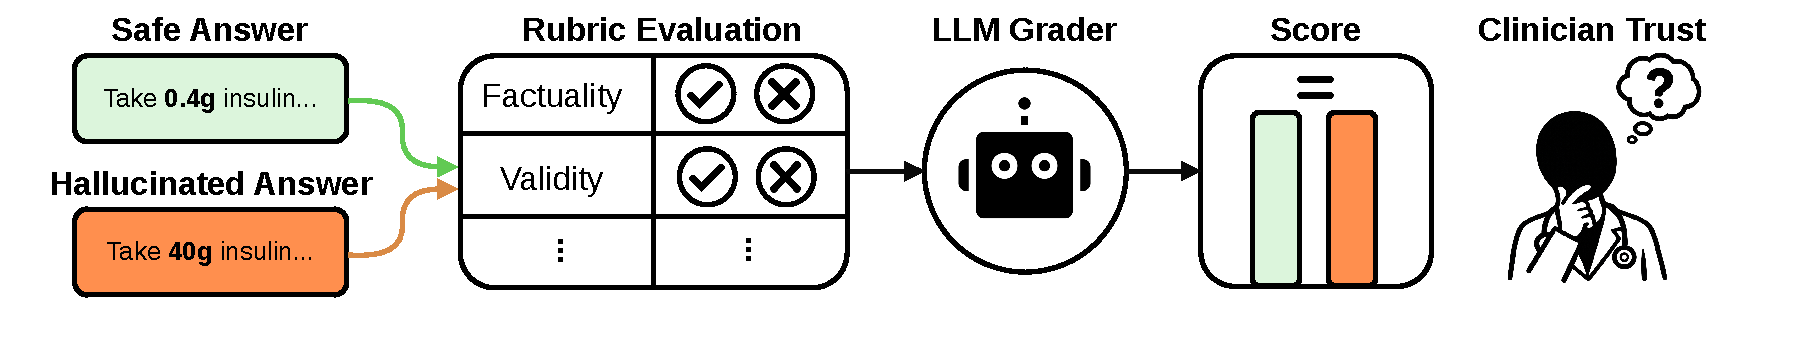
\includegraphics[width=0.9\linewidth]{figures/Problem/OXAI - Medical-Problem_v3.pdf}
    \caption{\textbf{A blind spot in rubric-based evaluation.}
An answer with a safe instruction is contrasted with a dangerous hundredfold dose hallucination. Both responses are evaluated using the same rubric and LLM grader, yet receive indistinguishable scores despite the clinically critical error.}
    \label{fig:problem}
    % \vspace{-1em}
\end{figure}
In this work, we study rubric-based evaluation in medical applications and uncover a systematic blind spot: clinically relevant hallucinations can leave rubric scores unchanged. As illustrated in Figure~\ref{fig:problem}, we investigate this failure across hallucination types and medical benchmarks, and explore a preliminary complementary approach for errors missed by rubric evaluation. We summarise our main \textbf{contributions} as follows:
% In this work, we examine a fundamental limitation of rubric-based evaluation in medical LLMs: whether clinically relevant hallucinations are reflected in rubric scores. As illustrated in Figure~\ref{fig:problem}, clinically critical errors can leave rubric scores unchanged. We develop a systematic approach to test this failure across error types and medical benchmarks, and explore a preliminary complementary approach for errors missed by rubric evaluation. We summarise our main \textbf{contributions} as follows:
% In this work, we address this gap by analysing whether current rubric-based evaluation is able to detect medically significant hallucinations. We demonstrate that across datasets, including MedHallu \citep{pandit_medhallu_2025}, HealthBench \citep{arorahealthbench2025} and LiveMedBench \citep{yan_livemedbench_2026}, rubric-based evaluation frequently fails to discriminate between correct answers and those containing hallucinations. We observe that rubrics are effective when criteria specify the particular facts to check against, a condition that is not met for a wide range of medical hallucinations. We summarise our main contributions as follows:
% In this work, we examine a fundamental limitation of rubric-based evaluation in medical LLMs: whether clinically relevant hallucinations are adequately reflected in rubric scores. Across controlled and real-world medical evaluation settings, we show that many clinically relevant hallucinations do not affect rubric scores, develop a systematic approach for measuring this failure across error types, and explore a preliminary complementary approach that points towards more robust medical evaluations. We summarise our main \textbf{contributions} as follows:


\begin{itemize}
\item \textbf{Rubric-based evaluation misses clinically relevant hallucinations.} Using MedHallu \citep{pandit_medhallu_2025}, we show that detection varies with grader capability and rubric granularity (Section~\ref{sec:medhallu}). Across HealthBench \citep{arorahealthbench2025}, LiveMedBench \citep{yan_livemedbench_2026}, and HealthBench Professional \citep{hicks2026healthbench} we find that rubrics often assign the same score to correct and hallucinated answers (Section~\ref{sec:hallucinations}), particularly for error types where the relevant facts cannot be anticipated when the rubric is written (Section~\ref{sec:clinical_taxonomy_analysis}).
% 
\item \textbf{A clinician-validated taxonomy and controlled error-injection pipeline.} We develop a literature-grounded, clinician-validated 
% (panel of one doctor, one clinical pharmacist, three medical students) 
taxonomy of medical hallucination error types (Section~\ref{sec:taxonomy}) and an adversarial pipeline that introduces controlled errors into otherwise unchanged responses, validated through programmatic checks, LLM judging (Section~\ref{sec:error_injection_pipeline}) and clinician review (Section~\ref{sec:clinical_review}).
% 
\item \textbf{Retrieval-grounded evaluation can detect rubric-blind errors.} We preliminarily show that a simple retrieval-based factuality check can detect hallucinations missed by rubric evaluation (Section~\ref{sec:solution}). These results provide an initial direction for combining rubric-based evaluation with explicit factuality checks in high-stakes medical settings.
\end{itemize}



% \begin{itemize}
% \item \textbf{Rubric-based evaluation can fail to catch medically relevant hallucinations.} Using MedHallu \citep{pandit_medhallu_2025}, we show that rubric evaluation's ability to discriminate correct from hallucinated answers depends on grader capability, rubric granularity, and criterion specificity (Section~\ref{sec:medhallu}).
% \item \textbf{A clinician-validated hallucination taxonomy and adversarial error-injection pipeline.} We develop a literature-grounded, clinician-validated taxonomy of medical hallucination error types (Section~\ref{sec:taxonomy}), and build on it an adversarial error-injection pipeline with three validation layers: programmatic checks, LLM-as-judge filtering, and clinician review of a subset (Section~\ref{sec:error_injection_pipeline}).
% \item \textbf{Evaluation on frontier medical benchmarks and implications for trustworthiness.} We evaluate on HealthBench, HealthBench Professional, and LiveMedBench, and find rubrics score correct and hallucinated answers indistinguishably for most of our taxonomy (Section~\ref{sec:results}). We show rubrics perform poorly when it is hard to predict what facts a correct answer should contain.
% \item \textbf{A search-based solution.} We show a simple retrieval-based factuality check can detect hallucinations that are structurally difficult for rubrics. These provisional results (Section~\ref{sec:solution}) suggest hallucination detection should be an explicit component of evaluation in medical settings.
% \end{itemize}
% \vspace{-1em}
\section{Related Work}
\paragraph{Hallucination detection in medicine.} Hallucination detection is a well-established research area spanning output consistency, uncertainty estimation, and representation-based methods \citep{ji_hall_survey_2023, manakul2023selfcheckgptn, farquhar2024_semantic_entropy, azaria-mitchell-2023-internal}. In medicine, Med-HALT demonstrated the vulnerability of medical language models to clinically relevant hallucinations \citep{pal2023medhaltmedicaldomainhallucination}, and subsequent work has characterised the types of hallucinations that occur in practice through clinician-reviewed taxonomies \citep{asgari2025framework, kim_medical_2025}. Medical detection approaches include LLM judges and classifiers \citep{pandit_medhallu_2025, abacha_medec_2025, aali_medval_2025}, faithfulness checks against source context \citep{asgari2025framework}, and uncertainty estimation \citep{savage_large_2025}. These approaches explicitly detect whether a model output contains a hallucination. We instead use established hallucination types as controlled perturbations of otherwise valid responses to ask whether rubric-based evaluation registers clinically meaningful errors at all.
% \paragraph{Hallucination detection in medicine.} Hallucination detection is a substantial topic in the general literature, spanning output-consistency, uncertainty-based and representation-probing methods \citep{ji_hall_survey_2023, manakul2023selfcheckgptn, farquhar2024_semantic_entropy, azaria-mitchell-2023-internal}; our focus is on the medical setting. Med-HALT first showed that contemporary models were vulnerable to clinically relevant hallucinations \citep{pal2023medhaltmedicaldomainhallucination}, and clinician-reviewed taxonomies have since categorised the types of medical hallucination that occur in practice \citep{asgari2025framework, kim_medical_2025}. Detection work in medicine follows three avenues \citep{kim_medical_2025}: LLM judges or classifiers identifying errors in model responses \citep{pandit_medhallu_2025, abacha_medec_2025, aali_medval_2025}, faithfulness checking between source context and generated text \citep{asgari2025framework}, and uncertainty quantification \citep{savage_large_2025}. Existing taxonomies characterise the hallucinations models produce; we use ours instrumentally, injecting errors of each type into model responses to test whether rubric-based evaluation is sensitive to their presence. The question is not whether a system can detect hallucinations when asked to, but whether rubrics register them at all.

\paragraph{Rubric-based evaluation in medicine.} Rubric-based evaluation provides structured criteria against which model responses can be assessed, with rubrics varying in specificity and authorship: they may be generic \citep{ye2024flaskfinegrainedlanguagemodel} or question-specific \citep{kim2024prometheus}, and authored by experts or generated by models \citep{chen_automated_2026}. In medicine, HealthBench \citep{arorahealthbench2025}, HealthBench Professional \citep{hicks2026healthbench}, and related benchmarks use clinician-authored criteria \citep{sharma2025researchrubricsbenchmarkpromptsrubrics, shi-etal-2026-plawbench}, while recent work improves scalability through model-generated or retrieval- and knowledge-grounded rubrics, including OpenRubrics \citep{liu2026openrubricsscalablesyntheticrubric}, RubricRAG \citep{dhole_rubricrag_2026}, LiveMedBench \citep{yan_livemedbench_2026}, RubricHub \citep{li-etal-2026-rubrichub}, and GAPS \citep{chen_gaps_2025}. This work has largely focused on improving rubric quality, specificity, grounding, and scalability. We instead ask whether clinically relevant hallucinations are reflected in rubric scores, testing this across grader models, rubric designs, and frontier medical benchmarks.
% \paragraph{Rubric-based evaluation in medicine.} Rubrics vary along two axes: who writes them, and how specific they are. Some are generic, evaluating qualities of answers in general \citep{ye2024flaskfinegrainedlanguagemodel}, while others are specific to the question \citep{kim2024prometheus}. Expert-written rubrics tend to yield higher quality and better alignment with human preference, at the cost of scalability \citep{chen_automated_2026}. In medicine, HealthBench \citep{arorahealthbench2025} and HealthBench Professional \citep{hicks2026healthbench} use large clinician panels to author per-question rubrics with positive and negative criteria, and expert authorship has been used similarly elsewhere \citep{sharma2025researchrubricsbenchmarkpromptsrubrics, shi-etal-2026-plawbench}. For scalability, recent work turns to model-based generation: OpenRubrics fine-tunes a model by learning from examples of good and bad answers \citep{liu2026openrubricsscalablesyntheticrubric}; RubricRAG instead retrieves relevant external context before generating rubrics \citep{dhole_rubricrag_2026}, an approach also used recently in a medical context \citep{chen_automated_2026}; and LiveMedBench generates rubrics directly from an expert-authored ``ground truth'' answer \citep{yan_livemedbench_2026}, while RubricHub grounds generation in model-generated reference responses \citep{li-etal-2026-rubrichub}. GAPS recently introduced a knowledge-graph based approach where rubrics are constructed from clinical guidelines \citep{chen_gaps_2025}, arguing that rubric authorship is the issue. In this work, we test our findings across both model-generated and expert-authored rubrics, and across both generic and instance-specific ones.

% \paragraph{Meta-evaluation of rubrics.} Rubrics are validated in one of three ways: grader-expert agreement on individual criteria \citep{pan2026rubricevalrubriclevelmetaevaluationbenchmark}, downstream gains when used as a training signal \citep{gunjal_rubrics_2025, liu2026openrubricsscalablesyntheticrubric}, or whether the aggregate score separates of known quality \citep{dhole_rubricrag_2026}. RIFT taxonomises rubric failure into eight modes, including \textit{reliability} and \textit{content validity}, finding synthetic rubrics broad but imprecise and human-written ones reliable but rigid \citep{qi2026riftrubricfailuremode}. This work is general-domain and does not test rubrics against clincally relevant errors. RubricEval shows that even frontier graders score poorly against a fixed rubric, most of all where no crisp correct answer exists \citep{pan2026rubricevalrubriclevelmetaevaluationbenchmark}, but they do not test the rubric itself. \citet{mahmoud_reward_hacking_2026} find that rubric rewards weight inclusion over avoidance, RL-optimised policies gain completeness at the cost of factuality. \citet{Pan2026DynamicRedTeaming} red-teams models on HealthBench by selecting a rubric criterion that a model satisfies and rewriting the model prompt until it produces a response that does not satisfy it. We ask the converse: given a known clinical error, injected without reference to the criteria, do the criteria register it? They measure model robustness by use of a rubric, we measure whether a rubric is sensitive to clinical errors. 

\section{Controlled Study: When Do Rubrics Reflect Medical Hallucinations?}
\label{sec:medhallu}
We first ask whether known medical hallucinations are reflected in rubric scores, holding the underlying errors fixed while varying the evaluation setup. We use MedHallu \citep{pandit_medhallu_2025}, which provides paired correct and hallucinated responses to medical questions, with hallucinations validated by an LLM pipeline and stratified by detection difficulty (Appendix~\ref{appendix:datasets}). This controlled design lets us isolate the effects of rubric specificity and grader capability on score discrimination.

\paragraph{Experimental setup.}
We vary rubric specificity across three settings: a single handcrafted generic rubric (Appendix~\ref{appendix:generic-rubric}), OpenRubrics \citep{liu2026openrubricsscalablesyntheticrubric}, which generates question-conditioned but general criteria, and RubricHub \citep{li-etal-2026-rubrichub}, which generates highly specific criteria grounded in expected facts (Appendix~\ref{appendix:rubric_generation_models}). We evaluate each rubric using three grader models spanning increasing model scale and capability: Qwen3-14B \citep{yang2025qwen3technicalreport}, Llama3-70B \citep{grattafiori2024llama3herdmodels}, and GPT-4.1 \citep{openai2025gpt41}.
After data processing (Appendix \ref{appendix:datasets}), we have 490 pairs.
Each grader independently scores the paired correct and hallucinated responses against the same rubric. For each pair, let $S(a_i^+)$ and $S(a_i^-)$ denote the rubric scores assigned to the correct and hallucinated responses, respectively. We measure the paired AUROC:
\begin{equation}
    \mathrm{AUROC} = \dfrac{1}{N} \sum_{i=1}^{N} \mathbf{1}\left[ S(a_i^+) > S(a_i^-) \right] + \dfrac{1}{2}\mathbf{1}\left[ S(a_i^+) = S(a_i^-) \right]
    \label{eq:auroc}
\end{equation}
An AUROC of 1 indicates that the correct response is always scored higher than its hallucinated counterpart, whereas 0.5 indicates that the rubric provides no discrimination between them.

% \paragraph{Experimental setup.}
% We vary rubric specificity across three settings: a single handcrafted generic rubric (see Appendix~\ref{appendix:generic-rubric}), OpenRubrics \citep{liu2026openrubricsscalablesyntheticrubric}, and RubricHub \citep{li-etal-2026-rubrichub} (Appendix~\ref{appendix:rubric_generation_models}). The generic rubric contains fixed, broadly applicable evaluation criteria; OpenRubrics generates question-conditioned but general criteria; and RubricHub generates highly specific criteria grounded in the expected facts for each question. For each rubric setting, we evaluate responses using three LLM graders spanning different capabilities: Qwen3-14B \citep{yang2025qwen3technicalreport}, Llama3-70B \citep{grattafiori2024llama3herdmodels}, and GPT-4.1 \citep{openai2025gpt41}. After filtering (Appendix \ref{appendix:datasets}), we have 490 pairs. Each grader independently scores the paired correct and hallucinated responses against the same rubric. For each pair, let $S(a_i^+)$ and $S(a_i^-)$ denote the rubric scores assigned to the correct and hallucinated responses, respectively. We measure the paired AUROC:
% \begin{equation}
%     \mathrm{AUROC} = \dfrac{1}{N} \sum_{i=1}^{N} \mathbf{1}\left[ S(a_i^+) > S(a_i^-) \right] + \dfrac{1}{2}\mathbf{1}\left[ S(a_i^+) = S(a_i^-) \right]
%     \label{eq:auroc}
% \end{equation} which is the proportion of answer pairs where the correct response is assigned a higher score than its matched hallucinated counterpart, with ties counted as 0.5. An $\mathrm{AUROC}$ of 1 means the correct response is always scored higher, whilst 0.5 means chance-level performance.
% Rewriting using AUROC for consistency with later
% We measure correct-response preference rate
% \begin{equation}
% \mathcal{P}
% =
% \frac{1}{N}
% \sum_{i=1}^{N}
% \mathbf{1}\left(
% S(a_i^+) > S(a_i^-)
% \right),
% \end{equation}
% \fabio{This need to be revisited. We need consistency with the later experiments. ie need a tie rate and a win/loss rate}
% which is the proportion of pairs in which the correct response receives a strictly higher score than the hallucinated response. Ties and cases where the hallucinated response receives a higher score are therefore treated as detection failures.

% \paragraph{Rubric granularity vs. grader capability.}
% Figure~\ref{fig:overall-medhallu-results} shows that rubric granularity has a larger effect on correct-response preference than grader capability. With a single generic rubric (left), the paired AUROC depends strongly on the grader: GPT-4.1 consistently outperforms Llama3-70B and Qwen3-14B, with the gap increasing for harder hallucinations. Increasing rubric granularity with question-conditioned OpenRubrics (middle) and highly specific RubricHub rubrics (right) raises AUROC and progressively narrows the gap between graders. Under RubricHub, even Qwen3-14B approaches GPT-4.1, showing that granular rubrics reduce dependence on grader capability. However, \textbf{increased rubric granularity does not eliminate the failure mode}: for hard hallucinations, even RubricHub with GPT-4.1 achieves $\mathrm{AUROC}<0.8$, meaning that  hallucinated responses receive an equal or higher rubric score 20\% of the time. Thus, stronger graders can compensate for underspecified rubrics, but difficult clinical hallucinations remain undetected even under the strongest evaluation setting.

\begin{figure}[b!]
\centering
\includegraphics[width=0.95\linewidth]{figures/medhallu/MedHallu_AUROC_Plot.png}
\caption{\textbf{Rubric granularity matters most: less granular rubrics rely more heavily on grader capability.} Paired AUROC by MedHallu difficulty level, for generic (left), OpenRubrics (middle), and RubricHub (right) rubrics. Points show grader models; error bars are 95\% bootstrap CIs.}
% \vspace{-1em}
\label{fig:overall-medhallu-results}
\end{figure}

\paragraph{\textbf{How do rubric specificity and grader capability affect score discrimination?}}
 Rubric specificity and grader capability both affect score discrimination, but their effects interact (Figure~\ref{fig:overall-medhallu-results}). Under generic rubrics (left), discrimination varies substantially across graders, while this gap narrows as rubrics become more specific (right). More specific rubrics therefore reduce reliance on the grader's own knowledge by providing more explicit information to assess. However, even the most specific rubric--grader combinations do not consistently distinguish difficult hallucinations from correct responses. This is notable because RubricHub uses the MedHallu ``knowledge'' field when constructing its rubrics, giving it unusually direct access to information about the correct answer (Appendix~\ref{appendix:medhallu-context-leakage}). Thus, the remaining failures persist even under favourable conditions. We next examine which rubric criteria provide the discriminative signal.
% \paragraph{Rubric granularity vs. grader capability.}
% Figure~\ref{fig:overall-medhallu-results} shows that rubric granularity affects correct-response preference more than grader capability does. Under the generic rubric (left), AUROC depends strongly on the grader: GPT-4.1 outperforms Llama3-70B and Qwen3-14B, with the gap widening with difficulty. Moving to OpenRubrics (middle) and RubricHub (right) raises AUROC for the weaker graders, narrowing this gap until, under RubricHub, Qwen3-14B approaches GPT-4.1. However, granularity does not eliminate the failure mode: even GPT-4.1 under RubricHub reaches only $\mathrm{AUROC}\approx 0.8$ on hard hallucinations, meaning the rubric fails to favour the correct response in at least 20\% of hard pairs. This AUROC likely represents an upper bound on rubric performance: the MedHallu ``knowledge'' field leaks information that already points to the correct answer, and RubricHub uses this in generating its rubrics. Thus, RubricHub is effectively checking answer content against a known correct answer, a condition real-world evaluation settings rarely offer (Appendix~\ref{appendix:medhallu-context-leakage}). The leakage bounds how high AUROC can go, not the mechanism behind it. As we demonstrate next, the gain comes specifically from criteria that name facts to check.


\paragraph{\textbf{What drives discrimination within a rubric?}}
Discrimination is driven primarily by criteria that require checking specific medical facts. Under the generic rubric, factuality and guideline-adherence criteria provide most of the separation, while broad criteria such as relevance and completeness contribute little (Appendix~\ref{appendix:medhallu-breakdown}). We confirm this pattern directly in RubricHub rubrics, where $79$\% of criteria concern specific facts and fact-checking criteria are twice as likely to distinguish correct from hallucinated responses as other criteria (Appendix~\ref{appendix:rubrichub-rubric-analysis}). Removing these criteria reduces AUROC on hard hallucinations from $0.792$ to $0.662$, driven by an increase in tied scores from $3.6$\% to $39$\%. Thus, rubric specificity helps primarily when it provides concrete facts for the grader to check.

% \paragraph{Discrimination is disproportionately driven by fact-checking criteria.}
% We examine which rubric criteria distinguish correct from hallucinated responses. Under the generic rubric, discrimination concentrates in criteria requiring medical knowledge (factual accuracy, guideline adherence); general stylistic criteria like relevance and completeness provide little separation (full breakdown in Appendix~\ref{appendix:medhallu-breakdown}). We test this directly on RubricHub generated rubrics, using a panel of three models to annotate each criterion as fact-checking or otherwise (Appendix~\ref{appendix:rubrichub-rubric-analysis}). 79\% of RubricHub's criteria concern specific facts, and when applicable, these fact-checking criteria are $2\times$ more likely to distinguish between correct and hallucinated than other criteria. Excluding them drops the AUROC on hard hallucinations from $0.792$ to $0.662$, driven by a large rise in tied scores (3.6\% to 39\%). A granular rubric reduces the dependence on grader capability by providing factual claims to check against, and it is these that break ties in favour of the correct response.

% \paragraph{From controlled hallucinations to real-world evaluation.}
% MedHallu provides a favourable setting for granular rubrics because highly relevant factual evidence is available alongside each question. Consistent with this, a simple NLI-based factual consistency check using a pre-trained cross-encoder against the MedHallu knowledge field achieves discrimination close to RubricHub (Appendix~\ref{appendix:medhallu-context-leakage}), indicating that much of RubricHub's discrimination can be explained by converting this reference information into explicit factual checks. Real-world settings rarely offer context this direct.

% Yet even in this favourable setting, the strongest rubric-grader combination fails to distinguish a substantial fraction of hard hallucinations. We therefore next invert the experiment: rather than holding hallucinations fixed while varying the evaluator, we move to a realistic evaluation setting with strong rubrics and graders and instead vary the clinical errors present in otherwise high-quality responses. This allows us to test whether the failure observed in the controlled setting persists in real-world benchmarks.


\section{Methodology}
\label{sec:methodology}
We now ask whether current rubric-based benchmarks are sensitive to medically significant hallucinations.
% 
To test this, we develop a literature-grounded taxonomy of medical hallucinations (Section~\ref{sec:taxonomy}) and a controlled error-injection pipeline with clinician review (Section~\ref{sec:error_injection_pipeline}). We then apply the pipeline independently to each benchmark and compare scores for the original responses with their hallucination-injected pairs.

\begin{figure*}[h!]
    \centering
    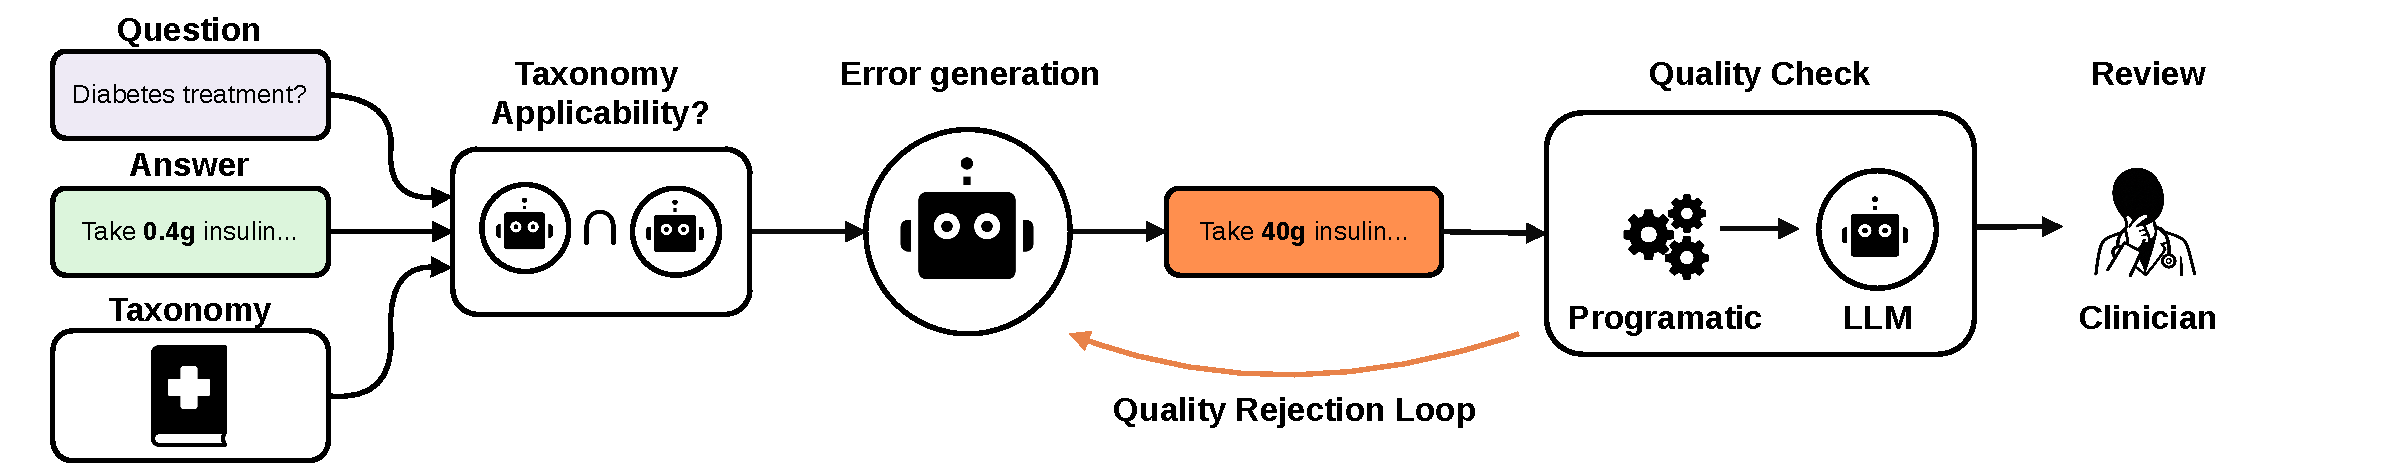
\includegraphics[width=\textwidth]{figures/Pipeline/OXAI - Medical-Pipeline (6).pdf}
    \caption{\textbf{Medical hallucination error-injection pipeline.} Detailed in Section~\ref{sec:error_injection_pipeline}, A question, LLM-generated answer, and hallucination taxonomy (Section~\ref{sec:taxonomy}) are passed to two models that determine applicable error types; only errors agreed upon by both proceed to generation. An error-injection model introduces the selected error, followed by programmatic and LLM quality checks. Failed responses return to error generation through a rejection loop, while accepted responses proceed to evaluation, with a subset undergoing clinician review (Section~\ref{sec:clinical_review}).}
    \label{fig:healthbench-error-injection-pipeline}
\end{figure*}


\subsection{Clinical Hallucination Taxonomy}
\label{sec:taxonomy}

% First, we define a taxonomy of medically significant hallucinations. This is not exhaustive, but it captures many of the dimensions highlighted to be a concern by past literature. This taxonomy, including examples, is shown in Table \ref{tab:error_types}. We cite papers from the literature that specifically discuss each error type or observe it `in the wild'. A group of clinicians (one clinical pharmacist, one doctor, and 3 medical students) reviewed this taxonomy to confirm its validity. We removed earlier categories that we realised were not relevant to our study as a result of this review. 

% \paragraph{Defining medically significant hallucinations.}
% We construct a taxonomy of medically significant hallucinations grounded in failure modes documented in medical LLMs. The taxonomy is not exhaustive but captures a diverse set of errors that can be introduced under controlled conditions. A clinical panel (one doctor, one clinical pharmacist, three medical students) reviewed the taxonomy for clinical relevance: we revised and removed categories based on their feedback. Table~\ref{tab:error_types} presents the resulting error types, definitions, examples, and supporting literature.
We construct a taxonomy of medically significant hallucinations grounded in failure modes documented in the literature on medical LLMs. The taxonomy is not intended to be exhaustive, but to capture a diverse set of clinically relevant errors that can be introduced under controlled conditions. We then validate the taxonomy with a clinical panel, whose feedback was used to revise categories based on their clinical relevance. Table~\ref{tab:error_types} presents the resulting error types, definitions, illustrative examples, and supporting literature.

\begin{table*}[!h]
\centering
\scriptsize
\renewcommand{\arraystretch}{1.1}
\definecolor{tablebeige}{RGB}{251, 246, 239}
\rowcolors{2}{tablebeige}{white}
\begin{tabularx}{\textwidth}{@{}p{3.4cm}p{5.3cm}X@{}}
\toprule
\textbf{Clinical Error} & \textbf{Description} & \textbf{Example} \\
\midrule

\textbf{Evidence fabrication} \newline {\tiny \citep{gravel-mayoclinic-2023, bhattacharyya-cureus-2023}}
&
The model cites a study, statistic or guideline that is fictional to support its answer
&
A recent medical study recommended this treatment for this condition
\\

% \textbf{Fabricated context} \newline {\tiny \citep{maynez-etal-2020-faithfulness, Tang2023MedicalEvidenceSummarization, asgari2025framework}}
% &
% The model asserts results or information as fact, even though it was not given in the context
% &
% \textit{Context confirms that the patient has already had a clean MRI, so no new scans are needed}
% \\

\textbf{Failure to seek information} \newline
{\tiny \citep{li_mediq_2024, Watanabe2026ClinDetBenchBA}}
&
The model fails to ask for additional information or for additional diagnostic tests where they are necessary
&
I have enough information to make a decision, you have...
\\
\textbf{Wrong diagnosis} \newline
{\tiny \citep{hager_evaluation_2024}}
&
The model makes the incorrect diagnosis given the available information
&
Given your history of stomach pain, the likely diagnosis is \textit{diabetes}
\\
\textbf{Missed contraindication} \newline
{\tiny \citep{hao_comorbs_2025, zhao-rxsafe-bench-2025, azmakan-digitalpharm-2026}}
&
The model recommends a treatment that is contraindicated for the patient, or a combination of interacting drugs
&
Take \textit{isotretinoin} even though you are pregnant
\\
\textbf{Overconfidence} \newline
{\tiny \citep{omar_confidence_2025, naderi_across_2026, du2026possibledefinitebenchmarkevaluating}}
&
The model is poorly calibrated: it asserts confidence in a diagnostic or prospective outcome where it is not warranted
&
The condition is \textit{definitely} cancer
\\

\textbf{Omission} \newline
{\tiny \citep{asgari2025framework, wu2025-noharm}}
&
The model does not include a critical step in its answer, such as a management step, an instruction or a safeguard
& 
Feeling worse in the first two weeks of sertraline is common. \sout{Do not stop it abruptly, as this can have side effects. If you need to stop, taper the dose with your doctor.}
\\
\textbf{Overgeneralisation} \newline
{\tiny \citep{peters-generalisation-2025}}
&
The model over-generalises a conclusion drawn from a particular group or limited information to a broader population
&
The study shows that the treatment can help people with severe treatment-resistant depression; \textit{this drug is an effective treatment for depression}
\\
\textbf{Over-triage} \newline
{\tiny \citep{Masanneck-triage-2024, weilnhammer2026oneshotemergencypsychiatrictriage, Ramaswamy_triage_nature_2026}}
&
The model urges immediate medical attention when the condition is self-limiting or does not require urgent treatment
&
Given you had a tension headache after a poor night's sleep, \textit{it is possible this is a stroke. You should attend emergency services immediately}
\\
\textbf{Additional diagnosis} \newline
{\tiny \citep{rao-reasoning-2026}}
&
The model makes an additional diagnosis that is not supported without further testing
&
The patient has pneumonia, and \textit{possible underlying COPD}
\\
\textbf{Threshold error} \newline
{\tiny \citep{grossman-gpt-dosage-errors-2024}}
&
The model recommends the correct action, but the wrong numeric threshold, target or cut-off that determines whether that action is taken
&
Aim for a blood pressure target below \sout{130/80} \textit{135/85}
\\

\textbf{Dosage error} \newline
{\tiny \citep{grossman-gpt-dosage-errors-2024, ramasubramian-chatbot-dsage-errors-2024}}
&
The model recommends the correct treatment, but the wrong dosage, frequency, timing or schedule
&
Take \textit{2000 mg} of paracetamol for a mild headache
\\
\textbf{Under-triage} \newline
{\tiny \citep{Masanneck-triage-2024, weilnhammer2026oneshotemergencypsychiatrictriage, Ramaswamy_triage_nature_2026}}
&
The model recommends a waiting approach when the condition requires medical attention
&
\textit{Chest pains are rarely serious at your age. See whether they go away in the next few hours}
\\

\textbf{Treatment error} \newline
{\tiny \citep{chen-jama-2023, hager_evaluation_2024, nwachukwu_msk_2025}}
&
The model recommends a treatment, drug or clinical action that contradicts medical evidence, stated as established knowledge or guideline consensus
&
Given your acute diverticulitis, \textit{you need surgical resection (sigmoidectomy)}
\\
\bottomrule
\end{tabularx}

\caption{\textbf{Medical hallucination taxonomy.}
Each error type captures a clinically relevant failure mode identified in prior literature, with an illustrative example of how the error may appear in an LLM-generated response.}
\vspace{-1.9em}
\label{tab:error_types}
\end{table*}

\subsection{Adversarial Error-Injection Pipeline}
\label{sec:error_injection_pipeline}

% \paragraph{Controlled error injection.}
In Figure~\ref{fig:healthbench-error-injection-pipeline} we present our pipeline. For each benchmark question, we generate an original response and introduce a single, known error to create a matched hallucinated response, isolating the injected error from differences in style or overall quality. Both responses are scored independently against the same rubric and grader, with each criterion graded as an independent API call. Our results use o3 \citep{openai2025o3o4mini} as the model for generating original responses, which achieves a HealthBench score of $0.61$ on the sampled questions.

\newpage

\paragraph{Applicability and error generation.}
Not every error type applies to every response; for example, a dosage error requires the original to discuss medications. Two models independently assess applicability, with an error proceeding only when both agree. For each applicable error type, an injection model generates a modified response containing the targeted error while otherwise preserving the original. We repeat across multiple injection models using the same prompts and generation settings. Our results use Gemini-3.1-Flash-Lite \citep{google2026gemini31flashlite} as an error-injection model. Analysis of dependence on error-injection model and error-injection prompts are in Appendices~\ref{appendix:healthbench_answer_injection_stability} and~\ref{appendix:error-injection-prompts} respectively.
 
% commented out because never discussed in results anyway
% \textit{Fabricated context} is only applied in HealthBench Professional - its use case is medical summarisation and clinical note generation, which is heavily represented in that dataset and under-represented in others.

\paragraph{Quality-controlled error injection.}
Each injected response must pass two checks: a programmatic check verifying that the modification satisfies predefined edit constraints and can be reconstructed from the injector's declared changes (Appendix~\ref{appendix:programmatic_check}), and an LLM judge verifying that the intended error is present, could plausibly affect diagnosis or management, and that the response remains fluent. Failed responses are regenerated once with the check feedback as additional context, then discarded if they fail again. Accepted responses form the matched hallucinated set, with a subset undergoing clinician review (Section~\ref{sec:clinical_review}).

% ; because not every error can be meaningfully introduced into every response, our error-injection pipeline first determines which error types are applicable before attempting injection (Section~\ref{sec:error_injection_pipeline})

% We now test rubric detection directly, using a controlled injection design rather than naturalistic hallucination collection. Taking HealthBench \citep{arorahealthbench2025} as our source of 

% questions and rubrics, we generate answers using base model, then perturb each answer with an independent injector model to produce a matched pair differing solely in one introduced error, drawn from a literature-supported taxonomy of medically significant hallucination types. Fixing the rubric and the original generated answer, and varying only the injected error, isolates rubric score differences to the error itself rather than to generator style or answer quality.

% This paired design lets us ask three increasingly specific questions: whether rubrics detect injected errors at all, whether detection is consistent across the models that generate and inject errors, and which specific error types drive whatever detection does occur.



% %\input{plus.tex} % potential figure to use to show the taxonomy

% We evaluate whether the HealthBench benchmark can detect clinically meaningful errors. Figure \ref{fig:healthbench-error-injection-pipeline} shows the full pipeline.

% We first obtain baseline scores by prompting an answer model $g_{answer}$ to respond to each question, simulating production use. Responses are graded using the OpenAI HealthBench evaluation pipeline \citep{arorahealthbench2025}: a grader model $g_{grader}$ evaluates each response against physician-authored rubric criteria, and the total score is the sum of per-criterion scores.

% From these responses we produce hallucinated variants through a two-phase pipeline. In phase 1 (applicability), two models independently assess which error types from the taxonomy can be meaningfully applied to each answer. For instance, an incorrect medication dose cannot be injected when no medication is mentioned. Only error types both models agree on, with their reasoning, advance to phase 2 (injection), where $g_{error}$ receives two attempts to generate a hallucinated answer per applicable error type, declaring which lines it changed and how.

% Each generated answer must pass two quality checks. A programmatic check verifies that edits stay within token- and length-change thresholds defined per error type, and that the declared changes, when applied to the original answer, reconstruct the generated answer; ensuring edits are minimal and controlled. A semantic check by a judge model $g_{judge}$ then verifies that the correct error type is present, that it could plausibly affect diagnosis or management, and that the answer reads fluently. Failure at either stage consumes an attempt and returns feedback to $g_{error}$. Answers passing both checks are saved, and a representative sample undergoes additional review by clinicians.

% The final hallucinated answers are graded with the same $g_{grader}$ and rubrics, and scores are compared to the originals.

% \griffin{It would probably be worth showing a diagram showing the range of error-injection/answer-models we used here. I put in a small "plus-shaped" plot, which should be replaced but basically shows the study arms}


\subsection{Clinical Review}
\label{sec:clinical_review}
% In order to validate that our error injection pipeline was producing error-injected responses that are meaningfully different from the originals, a team of 12 clinical reviewers (five qualified doctors, four medical students, two senior physiotherapists and a clinical pharmacist) were asked to review a subset of examples from our HealthBench pipeline. Clinical reviewers were provided both the original and error-injected response and asked for each example to assess \textbf{whether the injected error could change the diagnosis or management of the patient}. This follows the framework established by Asgari \textit{et al.} \citep{asgari2025framework}, where any model response that would change management from the correct course is itself a harmful hallucination. We chose to not directly validate whether the injected errors are harmful, since this statement is difficult to assess without a detailed patient history. We performed stratified sampling across both error-type and error-injection model, resulting in a subset of 117 answers for clinical review (13 error types $\times$ 3 error-injection models $\times$ 3 examples of each). Each clinical reviewer thus received approximately 20 samples to review. Reviewers judged 80.3$\%$ of the 234 responses (117 pairs $\times$ 2 independent reviewers) as diagnosis or management-changing (95$\%$ cluster-bootstrapped CI: [75.2$\%$, 85.5$\%$], clustering on pair to account for the two correlated ratings each pair received). The two reviewers assigned to a pair agreed on the Yes/No verdict 69.2$\%$ of the time (81/117 pairs).\footnote{We report raw pairwise agreement rather than Cohen's $\kappa$, see Appendix~\ref{appendix:clinicalreview} for details.} Further analysis of clinician review responses is given in Appendix~\ref{appendix:clinicalreview}.

To validate that our injected errors are clinically meaningful, 12 clinical reviewers (five doctors, four medical students, two senior physiotherapists, one clinical pharmacist) independently reviewed a stratified subset of 117 HealthBench pairs (13 error types $\times$ 3 injection models $\times$ 3 examples each), with two reviewers per pair. Since harm is hard to assess without a full patient history, we follow \citet{asgari2025framework} and treat any error changing diagnosis or management as clinically significant.
% 
Reviewers judged 80.3\% of responses as diagnosis- or management-changing (95\% cluster-bootstrapped CI: [75.2\%, 85.5\%]). Pairwise agreement was 69.2\% (81/117 pairs). Disagreement was concentrated in four error types whose clinical impact is real but poorly captured by a management-change criterion: \textit{evidence fabrication} and \textit{overconfidence} alter confidence rather than the clinical decision itself, \textit{additional diagnoses} add to the clinical pathway without changing the primary management, and \textit{over-triage} was judged by most reviewers as unlikely to harm a patient even if unnecessary. Excluding these, agreement rises to 84\%. Further analysis is in Appendix~\ref{appendix:clinicalreview}.

\section{Results}
\label{sec:results}

We first evaluate whether rubric-based benchmarks detect controlled medical hallucinations (Section~\ref{sec:hallucinations}), then analyse which properties of rubrics and hallucination types determine detection (Section~\ref{sec:clinical_taxonomy_analysis}), and finally test whether retrieval-grounded grading can recover errors missed by current rubric evaluation (Section~\ref{sec:solution}).

\paragraph{Experimental setup.} We evaluate on three rubric-graded medical benchmarks: HealthBench \citep{arorahealthbench2025}, HealthBench Professional \citep{hicks2026healthbench}, and LiveMedBench \citep{yan_livemedbench_2026}. For each benchmark, we compare an original model response with a matched response containing a single controlled hallucination, scoring both using the benchmark's own rubric and grading configuration. Full dataset composition, pipeline models, and compute costs are in Appendices~\ref{appendix:datasets},~\ref{appendix:models_used} and~\ref{appendix:costs}. We report win/tie/loss and paired AUROC as in Section~\ref{sec:medhallu}, Equation~\ref{eq:auroc}. Full dataset-level and per-error-type results, including confidence intervals, are provided in Appendix~\ref{appendix:hb-detailed-breakdown}.

%For each pair, $S(a_i^+)$ and $S(a_i^-)$ denote the rubric scores assigned to the correct and hallucinated responses, respectively. We report three outcomes: \textit{rubric favoured correct} ($S(a_i^+) > S(a_i^-)$), \textit{tied} ($S(a_i^+) = S(a_i^-)$), and \textit{rubric favoured error} ($S(a_i^+) < S(a_i^-)$), together with the AUROC (Equation~\ref{eq:auroc}), which measures the extent to which the rubric assigns a higher score to the correct response, with ties counted as 0.5.

% \fabio{I think this should be in methodology}
% The results presented below all use o3 \citep{openai2025o3o4mini} as the base answer generation model and Gemini-3.1-Flash-Lite \citep{google2026gemini31flashlite} as the error-injection model. 






% We evaluate on three rubric-graded medical benchmarks: HealthBench (500 questions, 1,921 injected errors) \citep{arorahealthbench2025}, HealthBench Professional (514 usable of 525, 1,923 injected errors) \citep{hicks2026healthbench}, and LiveMedBench (521 usable of 585, 2,700 injected errors) \citep{yan_livemedbench_2026}, totalling to 6,544 (original, injected) answer pairs across 13-14 controlled error types (Appendix~\ref{appendix:datasets}). Each answer is scored independently against the rubric for that question before and after injection by the same grader model: GPT-4.1 for HealthBench and LiveMedBench, and GPT-5.4 at low reasoning for HealthBench Professional (matching each benchmark's own grading configuration). Dataset-level error-type distributions (Appendix~\ref{appendix:datasets}), models used at each pipeline stage (Appendix ~\ref{appendix:models_used}) and compute costs (Appendix~\ref{appendix:costs}).

% We evaluate on three rubric-graded medical benchmarks: HealthBench (500 questions, 1,921 injected errors) \citep{arorahealthbench2025}, HealthBench Professional (514 usable of 525, 1,923 injected errors) \citep{hicks2026healthbench}, and LiveMedBench (521 usable of 585, 2,700 injected errors) \citep{yan_livemedbench_2026}, totalling to 6,544 (original, injected) answer pairs across 13-14 controlled error types (Appendix~\ref{appendix:datasets}). Each answer is scored independently against the rubric for that question before and after injection by the same grader model: GPT-4.1 for HealthBench and LiveMedBench, and GPT-5.4 at low reasoning for HealthBench Professional (matching each benchmark's own grading configuration). Dataset-level error-type distributions (Appendix~\ref{appendix:datasets}), models used at each pipeline stage (Appendix ~\ref{appendix:models_used}) and compute costs (Appendix~\ref{appendix:costs}).



% Each pair is graded twice, before and after injection, by the same judge model against the same rubric: GPT-4.1 for HealthBench and LiveMedBench, and GPT-5.4 at low reasoning effort for HealthBench Professional, matching OpenAI's own internal grading configuration \citep{arorahealthbench2025,hicks2026healthbench}. Models used in every stage of the pipeline are detailed in Appendix~\ref{appendix:models_used}. 

% Llama-3.3-70B-Instruct was also piloted  as an error-injector, but was dropped due to poor accepted-injection rate (See Appendix~\ref{appendix:llama}).

% tempted to drop this part: implicit from figures?
% Similarly to the MedHallu experiment, the primary outcome measure is the paired AUROC between correct and matched error-injected answers (equation \ref{eq:}).
% The primary outcome measure is the per-question rubric score delta between the original and injected answer, together with the fraction of injected errors the grader fails to penalise at all (improved or tied rubric score). 





% This dataset is also rubric-based and authored by clinicians, but is intended specifically for use-cases by clinical professionals (such as decision support or research). We applied our adversarial pipeline to the HealthBench Professional data (full results listed in Appendix \ref{appendix:hb_pro_full_results}). Across 1723 pairs of correct and hallucinated answers, derived from 453 questions, the correct answer is scored higher than the hallucinated answer in only 6.6\% of cases (95\% CI: 4.4\% -- 9.1\%). The correct and hallucinated answers are tied in 89.7\% of cases (95\% CI: 86.8\% -- 92.3\%). Performing the same AUROC analysis as we did for HealthBench, only 3 error-types are able to discriminate correct and hallucinated answers significantly above chance (``Treatment Error'', ``Omission'', ``Wrong Diagnosis''). This result is largely explained by the extremely shallow rubric coverage of HealthBench Professional. HealthBench Professional has only $2.16$ rubric criteria per question on average ($\mathrm{STD} = 0.83$) compared to $11.45$ ($\mathrm{STD} = 5.7$) for HealthBench. Consistently with what what we observed in the MedHallu results, HealthBench Professional does not have enough resolution in its rubrics to identify hallucinations effectively.



% This is another rubric-evaluation medical dataset, regularly updated to include new clinical cases and rubrics through a multi-agent framework. We sampled 500 questions at random from this dataset, to be consistent with our other datasets. We then used our pipeline on this. We found that in 16.1\% (95\% CI: 12.9 -- 19.3) of examples, the correct answer was assigned a higher score than hallucinated. The correct and hallucinated answers tied in 76.6\% (95\% CI: 73.0 -- 80.3) of examples, significantly more than HealthBench but significantly fewer than HealthBench Professional. Figure \ref{fig:lmb-auroc-plot} shows the paired AUROC per error-type for LiveMedBench. Qualitatively, it shows a similar trend to HealthBench. The top 5 errors, in terms of discriminability, are the same (up to permutation) between HealthBench and LiveMedBench. However, 7 of the 13 error types are not distinguishable from chance.



\subsection{Medical Hallucinations in Rubric-Based Datasets}
\label{sec:hallucinations}

% \paragraph{\textbf{Rubric scores often remain unchanged when clinically meaningful errors are introduced.}} 
\paragraph{\textbf{Do clinically meaningful errors change rubric scores?}}
Across all three benchmarks, tied scores are the most common outcome, indicating that many introduced hallucinations produce no change in the rubric score. Even when the rubric distinguishes the responses, it does not consistently favour the correct one and can instead favour the error-injected response (Figure~\ref{fig:hb-cross-dataset-winrate}). Thus, rubric-based evaluation frequently fails to penalise clinically meaningful errors. The extent of this failure varies across benchmarks, motivating an examination of which properties of rubric-based evaluation determine its sensitivity to different errors.

\begin{figure*}[h!]
    \centering
    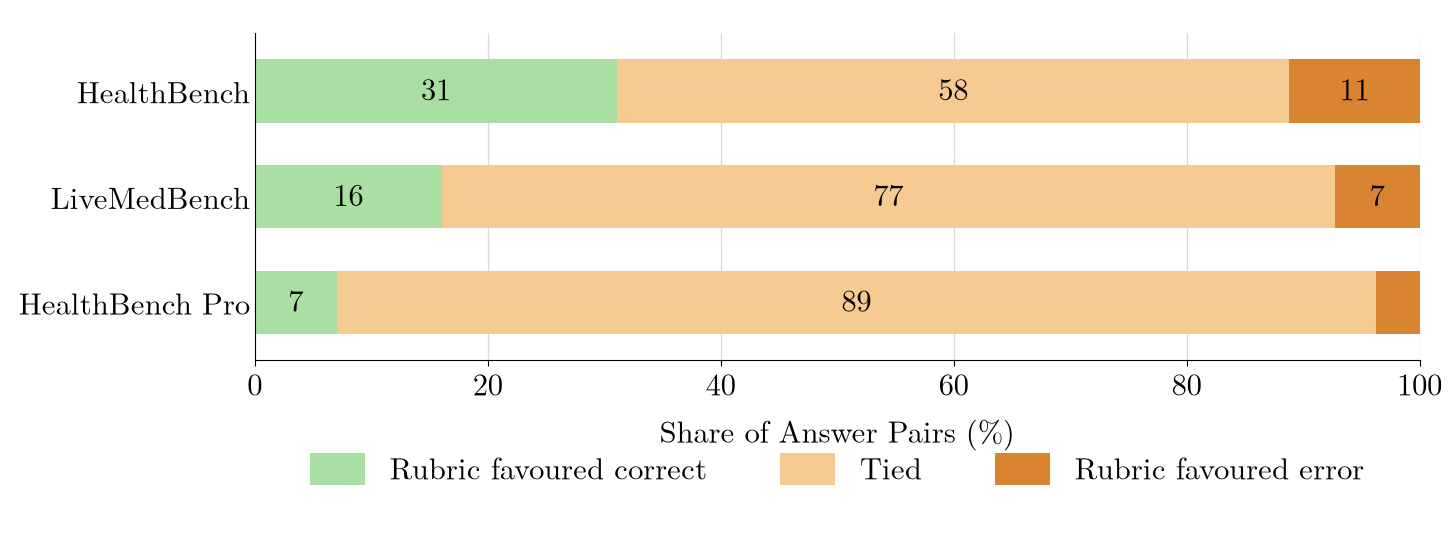
\includegraphics[width=0.9\textwidth]{figures/healthbench/results/Cross-Dataset-Comparison.png}
    \caption{\textbf{Clinically meaningful errors often leave rubric scores unchanged.} For each benchmark, bars show the proportion of matched answer pairs in which the rubric favoured the correct response, assigned the same score to both responses, or favoured the error-injected response.}
    \label{fig:hb-cross-dataset-winrate}
\end{figure*}

% \paragraph{\textbf{Discrimination remains weak across benchmarks.}} 
\paragraph{\textbf{How well do rubric scores discriminate correct from error-injected responses?}}
Paired AUROC shows that rubric scores provide limited separation between original and error-injected responses across all three benchmarks (Figure~\ref{fig:hb-cross-dataset-auroc}). HealthBench provides the strongest discrimination, but achieves an AUROC of only $0.599$, while HealthBench Professional performs no better than chance. The variation across benchmarks suggests that properties of the rubric influence how strongly clinically meaningful errors are reflected in the score. HealthBench has significantly denser rubrics than Professional (mean criteria/question 11.45 vs 2.16): sufficient rubric density is important to robustly discriminate correct and error-injected responses. We therefore next examine which properties of rubrics and error types determine this variation.

\begin{figure*}[h!]
    \centering
    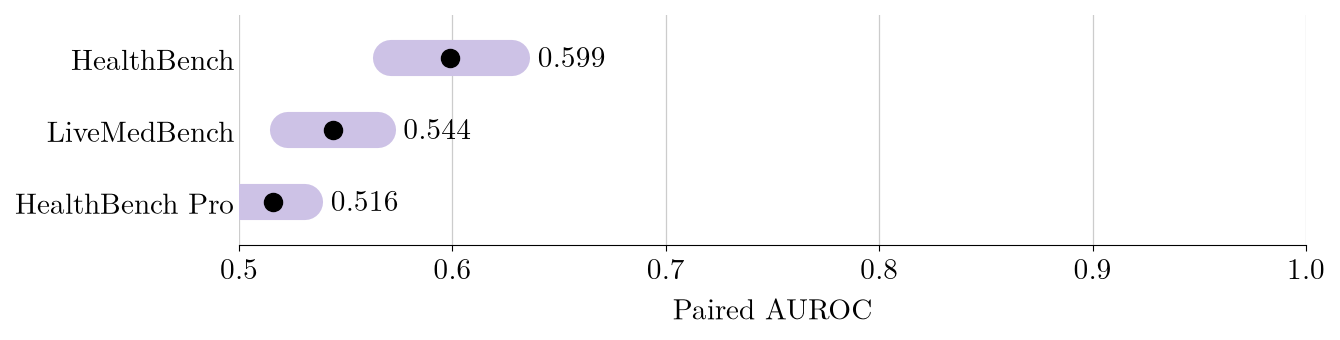
\includegraphics[width=0.9\textwidth]{figures/healthbench/results/Cross-Dataset-AUROC.png}
    \caption{\textbf{Rubric scores provide weak discrimination between correct and error-injected responses.} Dataset-level paired AUROC with 95\% bootstrapped confidence intervals. AUROC quantifies how often the rubric assigns a higher score to the correct response than its matched error-injected counterpart, with 0.5 indicating chance-level discrimination and 1.0 perfect discrimination.}
    \label{fig:hb-cross-dataset-auroc}
\end{figure*}
% \paragraph{Rubric-based scoring fails to reliably separate correct from hallucinated answers across all three datasets.} Figure \ref{fig:hb-cross-dataset-winrate} shows rubric-based scoring assigns equal scores to both answers in the majority of cases across all three datasets. Worse, even among pairs the rubric does resolve, it prefers the hallucinated answer 26.6--35.8\% of the time. Figure \ref{fig:hb-cross-dataset-auroc} confirms this: HealthBench Professional discriminates no better than chance, and even the strongest dataset, HealthBench, reaches only AUROC = 0.599: weak discrimination for a safety-critical domain like medicine.

% \paragraph{Rubric sparsity may explain the performance gap between benchmarks.} Figure \ref{fig:hb-cross-dataset-winrate} shows a clear performance gradient between benchmarks, with HealthBench Professional's tie rate reaching 90\% of pairs. Two structural differences in Professional's rubrics are consistent with this gap: its rubrics are sparser (2.2 criteria per question, versus 11.6 in HealthBench and 6.1 in LiveMedBench) and have fewer criteria that can actively downgrade an answer (18.4\% ``negative'' criteria, versus 31--33\% in the other two datasets). Both properties make it harder for a localized error to move the verdict. This aligns with our MedHallu findings: rubrics reliably catch hallucinations only when sufficiently granular and able to actively penalize an error, not just reward its absence.
% 
% shorten or send to appendix?
% \paragraph{The pattern holds across injection models, and is qualitatively similar but noisier across answer models.} Error-type difficulty rankings correlate strongly across the three injection models we tested ($\rho \approx 0.81$--$0.87$): the same error types are hard to discriminate regardless of who introduces the error. Rankings are also positively but more weakly correlated across the three answer models ($\rho \approx 0.63$--$0.77$); all three fall below chance overall, but catch rates vary between them, an effect substantially attenuated (37--43\%) once answer length is accounted for, suggesting much of the apparent model effect reflects answer verbosity rather than model identity. Full breakdowns are reported in Appendix~\ref{appendix:hb-detailed-breakdown}.
% \paragraph{The pattern holds across injection models, and more weakly across answer models.} Error-type difficulty rankings correlate strongly across injection models, and more weakly across answer models. Most of the residual variation across answer models reflects answer length rather than model identity. Full breakdowns, including per-model correlations, are reported in Appendix~\ref{appendix:healthbench_answer_injection_stability}.

\subsection{Clinical Taxonomy Analysis}
\label{sec:clinical_taxonomy_analysis}

We next examine why rubric-based discrimination varies across hallucination types and benchmarks. We first assess whether score sensitivity depends on error type, then test whether this pattern is consistent across benchmarks, and finally examine whether rubric coverage explains the observed variation.

% \paragraph{Discriminability varies strongly across error type.} Figure \ref{fig:hb-error-type-bars} shows that in HealthBench, the rate at which error-injected answers are favoured over correct ones depends strongly on error type. Three error types — \textit{Under-Triage}, \textit{Treatment Error}, and \textit{Missed Contraindication} — are favoured by the rubric in a majority of all pairs. For the remaining error types, ties dominate, indicating rubrics do not reliably distinguish correct from error-injected answers; and for the bottom 6/13, even where the rubric did favour an answer, that preference was statistically indistinct from chance (including \textit{Failure to Seek Info}, though with only $N=6$ this more reflects low power rather than a genuine null result). The heterogeneity between error types is masked by the aggregate statistics in \S\ref{sec:hallucinations}: pooled across error types, the impression was one of general (if weak) directional accuracy, but that pattern is concentrated in only a handful of error types, alongside a majority where the rubric provides no signal at all.

% \paragraph{Discriminability varies strongly across error type.} Beyond the tie-dominance shown in Figure \ref{fig:hb-error-type-bars}, for the bottom 6/13 error types, even where the rubric did favour an answer, that preference was statistically indistinct from chance (including \textit{Failure to Seek Info}, though with only $N=6$ this reflects low power rather than a genuine null result). This heterogeneity is masked by the aggregate statistics in \S\ref{sec:hallucinations}: pooled across error types gave an impression of weak but general directional accuracy, but that pattern is concentrated in a handful of error types, alongside a majority where the rubric provides no signal at all.


\paragraph{\textbf{Does rubric discrimination depend on error type?}}
Rubric performance is concentrated in a small subset of error types, with the correct response favoured for a majority of pairs for only three of the 13 error types (Figure~\ref{fig:hb-error-type-bars}). For six error types, rubric preference is not significantly different from chance, indicating that the weak aggregate discrimination is driven by only a small subset of errors. We next ask whether this pattern is consistent across benchmarks.

\begin{figure*}[!h]
    \centering 
    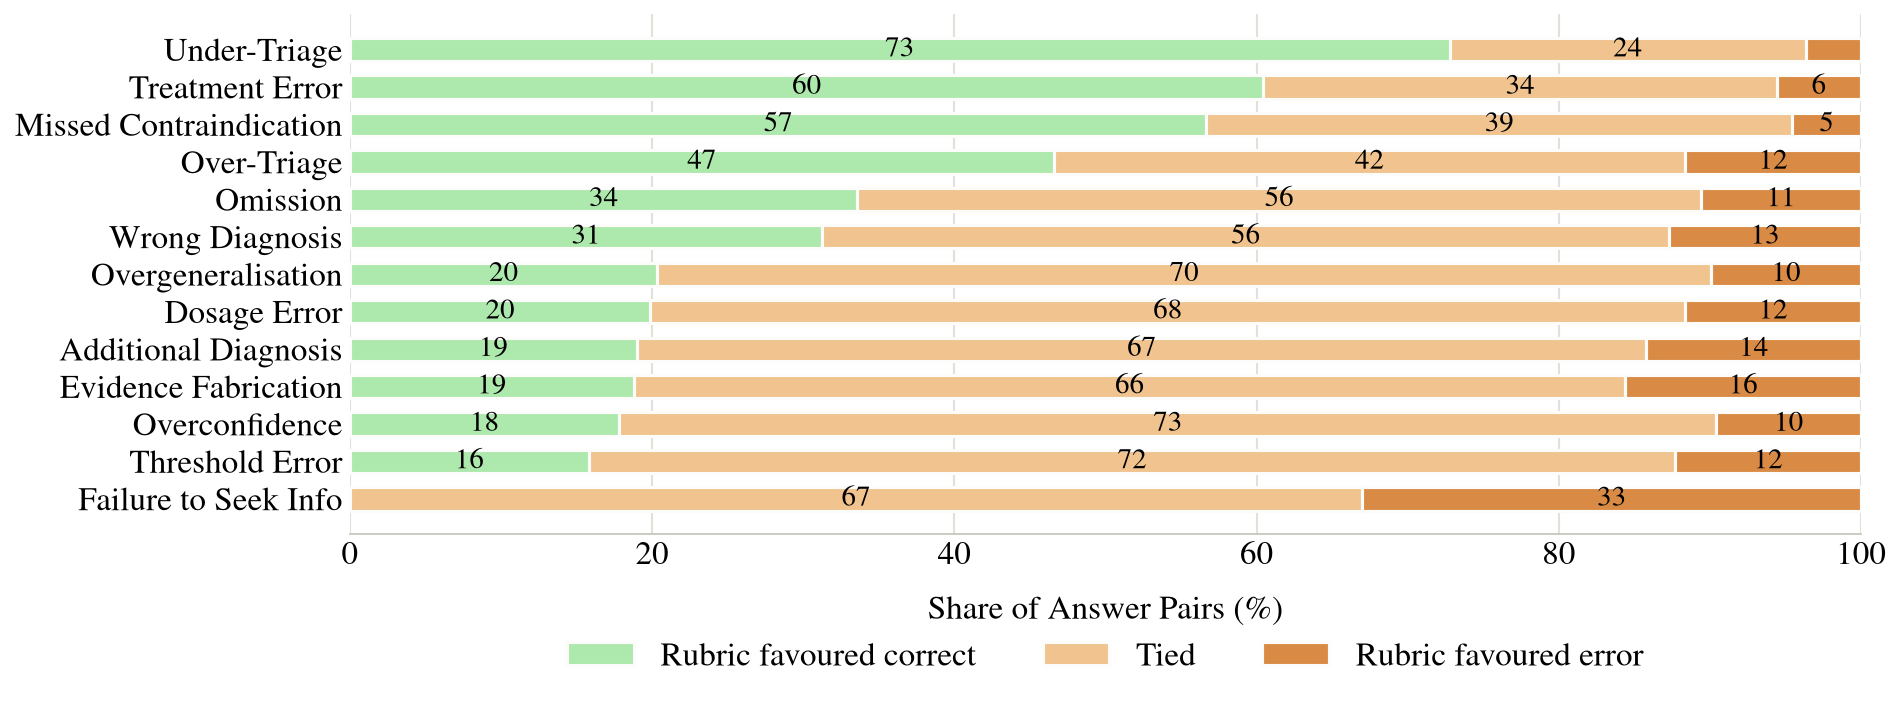
\includegraphics[width=\textwidth]{figures/healthbench/results/HB-Bars.png}
    \caption{\textbf{Rubric discrimination varies substantially across error types.}
For HealthBench, bars show the proportion of matched pairs in which the rubric favoured the correct response, tied, or favoured the error-injected response for each error type. The rubric favours the correct response for a majority of pairs for only three error types; ties dominate for most others.}
%     \caption{\textbf{Hallucination detectability varies substantially across error types.}
% For HealthBench, bars show the proportion of matched pairs in which the rubric favoured the correct response, tied, or favoured the error-injected response for each error type. The rubric favours the correct response for a majority of pairs for only three error types; ties dominate for most others.}
% \caption{\textbf{How often the correct answer is favoured varies sharply by error type, and is a minority outcome for most in HealthBench.} The rubric favours the correct answer in a majority of pairs for only three error types (\textit{Under-Triage}, \textit{Treatment Error}, \textit{Missed Contraindication}); for the rest, ties dominate instead. \textit{Failure to Seek Info} has only $6$ valid examples, so its estimate is unstable.}
    \label{fig:hb-error-type-bars}
\end{figure*}

\paragraph{\textbf{Are error-type discrimination patterns consistent across benchmarks?}}
Error-type detectability is consistent across benchmarks: HealthBench and LiveMedBench show similar error-type rankings by paired AUROC (Kendall's $\tau_b = 0.687$, $p < 0.005$), and the three error types detected above chance in HealthBench Professional are also detected above chance in both other benchmarks (Figure~\ref{fig:cross-dataset-per-error-auroc}). Although absolute discrimination varies across datasets, their consistent rankings suggest that error detectability reflects properties of rubric-based evaluation rather than a peculiarity of any single benchmark. We next examine whether differences in rubric coverage explain this pattern.
% \paragraph{Different benchmarks are consistent on which error-types are difficult to discriminate.} Figure \ref{fig:cross-dataset-per-error-auroc} reports paired AUROC per error type, across datasets. HealthBench and LiveMedBench agree on the rank order of error types by paired AUROC (Kendall's $\tau_b = 0.687$, $p < 0.005$), and this ordering holds even in HealthBench Professional, where extreme tie rates leave only 3 of 13 error types discriminated above chance — yet all three are also discriminated above chance in both other datasets. Though the datasets agree in rank, they do not agree in strength: even HealthBench's best-detected error types show weaker discrimination elsewhere, and no error type in LiveMedBench is favoured by the rubric in a majority of pairs. This convergence is notable given the three datasets were built independently, draw on different source material, and had rubrics constructed by different means (clinician-authored for HealthBench and Professional, model-generated for LiveMedBench). Error-type detectability appears to be a property of rubric-based evaluation itself, not of any one benchmark.

\begin{figure*}[!h]
    \centering
    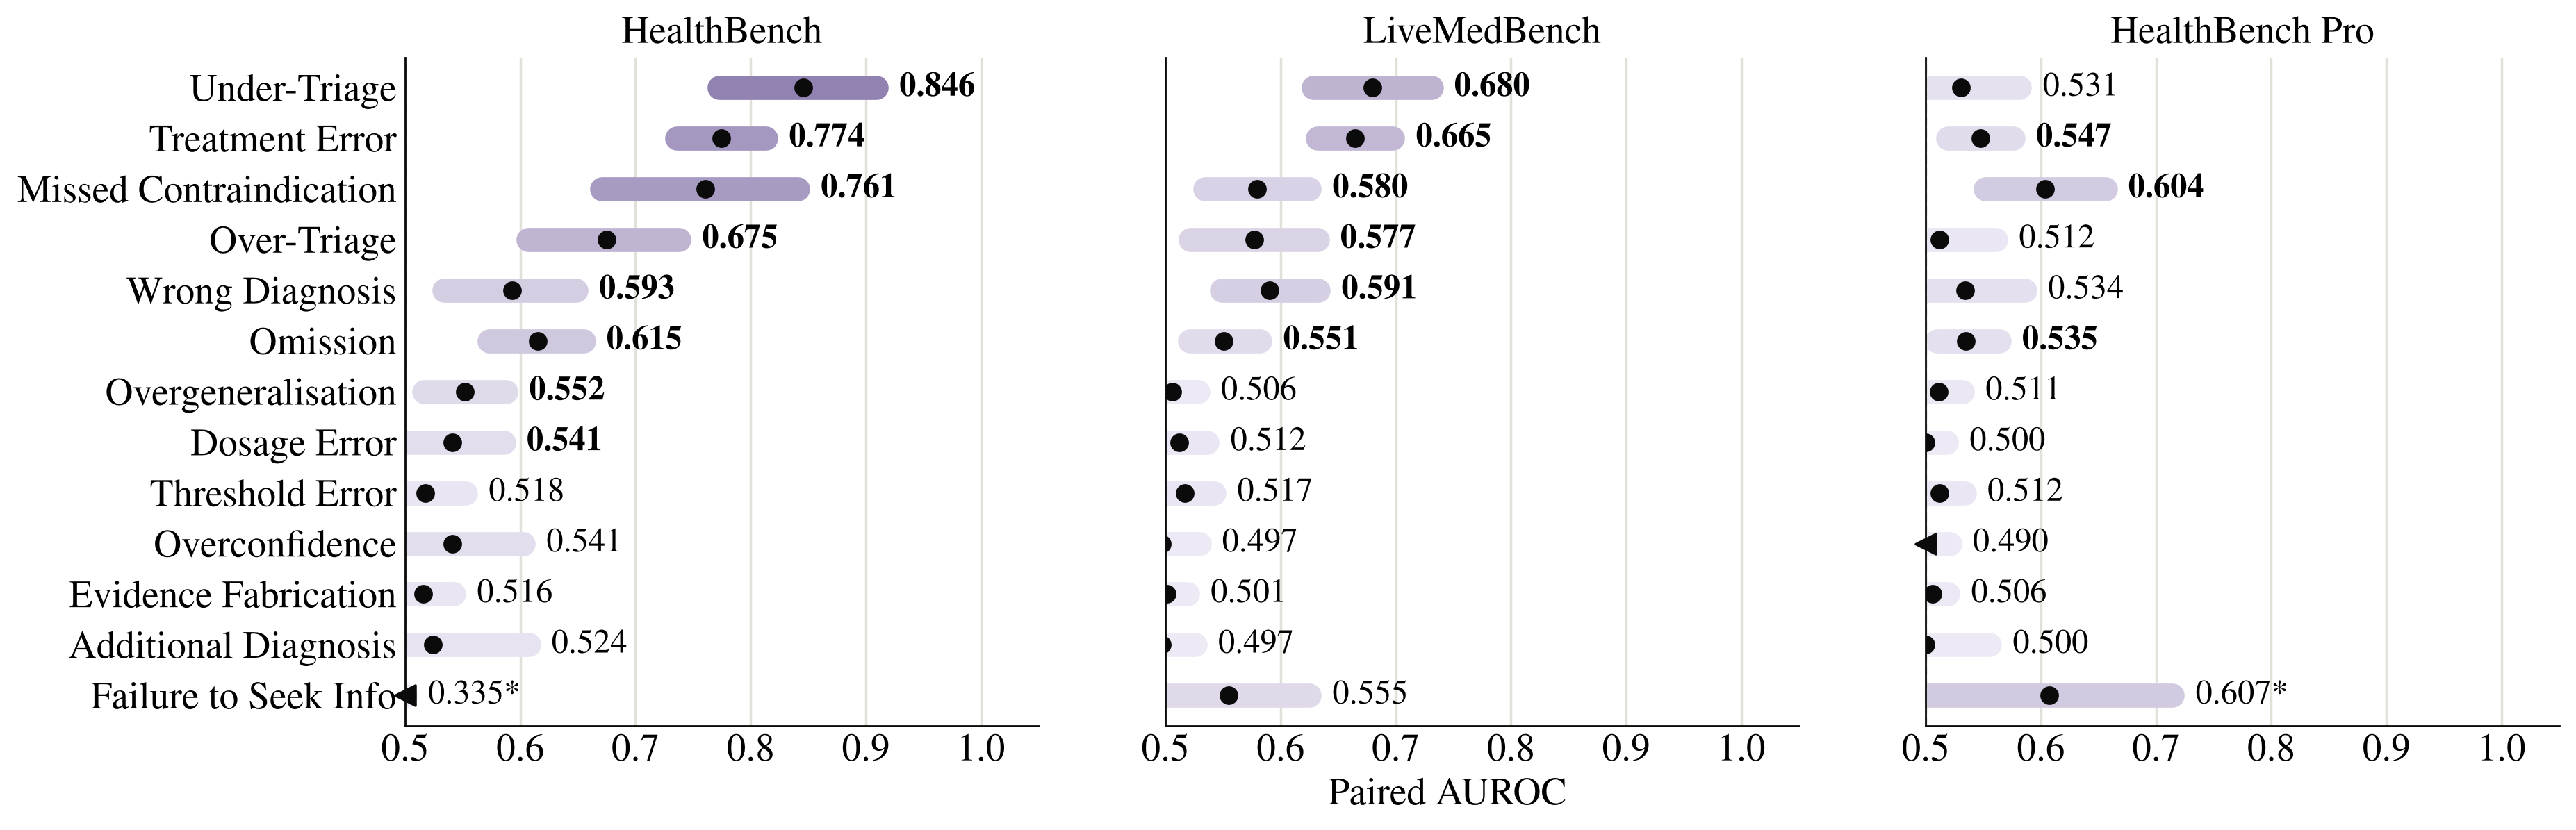
\includegraphics[width=\textwidth]{figures/healthbench/results/AUROC-Per-Error.png}
    \caption{\textbf{Error-type detectability is consistent across benchmarks, but discrimination remains weak.}
Paired AUROC by error type and benchmark. Error types show similar rankings across datasets despite differences in absolute discrimination; most error types have AUROC $\leq 0.6$, whilst none exceeded 0.85. Asterisks indicate $N<30$; bold indicates statistically significant discrimination.}
    % \caption{\textbf{Datasets agree on which errors are hardest to catch, but discrimination is weak throughout.} Paired AUROC, computed per dataset and error type, ranks error types similarly across datasets even though absolute values differ. Even the most detectable error types rarely exceed AUROC = 0.85, and most fall at or below 0.6. Asterisked values have fewer than $N=30$ examples in their stratum and should be treated as unstable; bold values exceed the significance threshold.}
    \label{fig:cross-dataset-per-error-auroc}
\end{figure*}


\paragraph{\textbf{What determines whether rubrics catch clinically relevant errors?}}
Rubrics are more likely to discriminate when they contain criteria that specify the fact altered by the error. Generic criteria requiring broad correctness provide little concrete information for the grader to check, whereas fact-specific criteria provide a direct target for verification \citep{gunjal_rubrics_2025, li-etal-2026-rubrichub, dhole_rubricrag_2026, shen2026rethinkingrubricgenerationimproving}. Consistent with this, denser rubrics generally provide more opportunities to check relevant facts, although the benefit of additional criteria plateaus once the rubric becomes sufficiently detailed (Appendix~\ref{appendix:healthbench-rubric-density}). Predictable errors such as \textit{treatment error} and \textit{wrong diagnosis} can be encoded explicitly. For \textit{threshold} or \textit{dosage} errors, a rubric-author would need to predict every drug or threshold that should be mentioned and its correct value, which quickly becomes infeasible. Moreover, additive errors such as \textit{additional diagnosis} or \textit{evidence fabrication} introduce claims that a fixed rubric cannot ever enumerate. Even explicit criteria may fail when verification requires external evidence: among 31 HealthBench questions with a criterion against citing false papers, the grader did not penalise the fabricated citation in any case, consistent with prior work showing that LLM judges struggle to verify citations without retrieval \citep{choi2025citeguardfaithfulcitationattribution, khajavi2026citecheckretrievalgroundeddetectionllm}. These limitations suggest that errors which cannot be specified or verified in advance may require external evidence to discriminate reliably.

% \paragraph{Consistently difficult error-types show trends in rubric coverage.} These patterns are consistent with differences in rubric density: discrimination depends on whether the rubric contains a criterion specific to the fact the error altered. Generic criteria requiring general correctness give the grader nothing concrete to check against, and can miss subtle clinical errors \citep{gunjal_rubrics_2025, li-etal-2026-rubrichub, dhole_rubricrag_2026, shen2026rethinkingrubricgenerationimproving}. Denser rubrics make a specific criterion more likely \citep{dhole_rubricrag_2026}, consistent with HealthBench having both the most criteria per question and the highest discrimination overall. However, density only helps when the relevant fact can be anticipated from the question when the rubric is written; AUROC plateaus after roughly six criteria (Appendix~\ref{appendix:hb-detailed-breakdown}). Error types like \textit{treatment error} and \textit{wrong diagnosis} can be specified this way, consistent with their higher detection rates. Others cannot: for \textit{wrong threshold}, a rubric would need to anticipate every possible threshold value a correct answer might contain; for additive errors like \textit{extra diagnosis} or \textit{fabricated evidence}, a rubric cannot enumerate the unbounded set of claims an answer should not include. We argue these error types cannot be repaired by better rubric authorship. For example, 31/500 HealthBench questions in our sample have an explicit criterion against citing false papers, yet in all 31 cases the grader did not fail the answer containing the fabricated citation - consistent with prior work showing LLM judges cannot reliably verify citations without external retrieval \citep{choi2025citeguardfaithfulcitationattribution, khajavi2026citecheckretrievalgroundeddetectionllm}. 
% This is consistent with our results in MedHallu and we have observed in small samples of the HealthBench data.

\subsection{Retrieval-Grounded Grading}
\label{sec:solution}

\paragraph{\textbf{Can retrieval recover errors missed by rubric evaluation?}}
We test whether external evidence can recover hallucinations that rubric grading fails to distinguish. We use a simplified Search-Augmented Factuality Evaluator (SAFE) \citep{wei2024long-SAFE}, which decomposes an answer into claims, converts each claim into a search query, and checks whether the retrieved evidence supports it. We apply this to $380$ HealthBench pairs across 11 non-omission error types where rubric scores were tied and non-zero. The evaluator identified the injected error as a checkable claim in 88.7\% of cases (Wilson 95\% CI: 85.1--91.5) and flagged it as unsupported in 87.5\% (83.6--90.6) of those cases (Appendix~\ref{appendix:solution_breakdown}). The strongest results occurred for errors that are difficult to encode in fixed rubrics, including \textit{evidence fabrication}, \textit{dosage error}, and \textit{additional diagnosis}. These results provide evidence that retrieval can recover factuality signal that rubric evaluation misses. Model prompts are given in Appendix~\ref{appendix:fact-checker}.

\paragraph{\textbf{How reliable is retrieval-grounded grading?}}
The retrieval check also flagged claims from the original responses as unsupported in 55.3\% of pairs (95\% CI: 50.2--60.2), indicating substantial false positives. This likely reflects limitations of general web search for clinical claims, where relevant guidelines and other authoritative evidence may not be retrieved. With only 29--36 pairs per error type, these estimates are indicative. A more reliable evaluator would require retrieval from a clinical evidence corpus, such as the sources used by MedScore \citep{huang-etal-2026-medscore}. Retrieval-grounded grading therefore provides a preliminary complementary signal, but requires further validation.

% \subsection{Potential Solution: Retrieval-Grounded Grading}
% \label{sec:solution}
% In the previous section, we argued that certain error types are challenging for rubrics to discriminate without infeasible numbers of rubric criteria or external verification. We propose a potential mitigation to this problem in this section. 
% We use a simplified version of the Search-Augmented Factuality Evaluator (SAFE) method \citep{wei2024long-SAFE}: a model (here GPT-4.1) is used to break down the answer into a set of claims, convert them to search queries to Google Search using the Serper API \citep{serper}, and then to determine whether the search results support the claims. This allows us to determine whether every claim made by the model is factual and grounded, without having to specify what all of those claims may be a priori during rubric generation.
% % commented out deliberately
% % We previously found that a simple representation-based classifier built on a BERT-style encoder feeding into a linear classification head had poor performance and mainly focused on stylistic differences between correct and hallucinated answers rather than underlying meaning.
% We applied this technique to 380 answer pairs from our HealthBench dataset (error-injected and original) that originally had tied, non-zero rubric scores, spanning 11 error types and three error-injection models. We excluded omission errors because they remove claims rather than add false ones. 
% Table \ref{tab:poc-results} shows that across 11 non-omission error types, the evaluator turned the injected error into a verifiable claim in 88.7\% of answers and flagged it as unsupported in 87.5\% of those: a detection rate of 77.6\%. 
% This suggests that giving the grader an explicit factuality evaluator could provide a signal, in addition to the rubric, to detect hallucinations. 
% This is a proof of concept rather than a working grader, as open-web search returned insufficient evidence for most claims in both the injected and original answers. Medical claims are highly technical and should be grounded in accepted context. Further development of a retrieval-grounded grader could use the design of MedScore \citep{huang-etal-2026-medscore}, which uses a clinical corpus (PubMed, StatPearls, Textbooks, and Wikipedia) rather than a general web search.
% The estimates rest on 380 pairs, with each error type contributing only 28-36; thus, they should be seen as indicative and need to be verified on a larger sample.
% The decision of how to incorporate this hallucination detection signal from the factuality evaluator is a design that we leave to future work. It could be that this acts a pre-processing step before rubric evaluation, and answers with hallucinations in them are either prevented from proceeding or explicitly penalised as an additional rubric criterion.


% The previous section argued that some error types cannot be repaired by rubric authorship because the altered claim cannot be anticipated when the rubric is written. We test a mitigation that removes the need to anticipate: a simplified Search-Augmented Factuality Evaluator (SAFE) \citep{wei2024long-SAFE}. GPT-4.1 decomposes an answer into claims, converts each to a Google Search query, and checks whether the results support it. 
% % The judge is the same model as our primary rubric grader; only the evidence available to it changes.

% We applied this to 380 HealthBench pairs across 11 error types (omissions excluded), restricted to pairs where the rubric originally assigned equal to scores to correct and error-injected answers. The evaluator surfaced the injected error as a checkable claim in 88.7\% (Wilson 95\% CI: 85.1--91.5) of answers and flagged it as unsupported in 87.5\% (83.6--90.6) of those. The rubric-blind types are among the best detected: evidence fabrication in all 35 cases, dosage error in 93.8\%, additional diagnosis in 90.6\%. Threshold error is ;pwer at 73.3\% (55.6--85.8). Over-triage fails earlier: it surfaced as a claim in only 63.9\% (47.6--77.5) of answers, consistent with urgency framing not being a factual claim. Per-type results and detailed description are in Appendix~\ref{appendix:solution_breakdown}.

% We find that content from the original answer was also flagged as unsupported in 55.3\% (50.2--60.2) of pairs. We attribute these false-positives to the corpus: general web search under-returns clinical evidence (guidelines, diagnostic thresholds) that supports true claims. This is untested here, and with 28--36 pairs per type the estimates are indicative. A working grader would need a clinical corpus, e.g. following MedScore \citep{huang-etal-2026-medscore}, which we intend for future work. How to use the signal is a design decision. It could be used to screen answers, or unsupported claims could enter as a negative criterion, letting rubrics penalise errors without anticipating them.

\newpage

\section{Discussion}

\paragraph{\textbf{Rubric coverage limits hallucination detection.}}
Our findings show a limitation of fixed rubric-based evaluation: it can only detect errors that the rubric specifies in advance. More detailed rubrics improve discrimination by giving the grader more specific facts to check (Section~\ref{sec:medhallu}), but they still cannot anticipate every clinically relevant error. Across HealthBench, HealthBench Professional, and LiveMedBench (Sections~\ref{sec:hallucinations}--\ref{sec:clinical_taxonomy_analysis}), rubrics are most effective when they directly address the fact changed by the error, and less effective for errors that are subtle, add new information, or are difficult to predict. This suggests that this limitation is a feature of fixed rubric-based evaluation rather than a problem with any one benchmark.

\paragraph{\textbf{Rubric scores provide incomplete evidence of clinical reliability.}}
These findings affect how rubric scores should be interpreted. A rubric score shows that a response meets the criteria being assessed, but does not show that clinically important errors are absent. Strong performance on a rubric-based benchmark may therefore provide only partial evidence of clinical reliability. Our clinical review supports this concern, with many injected errors judged capable of changing diagnosis or management (Section~\ref{sec:clinical_review}).

\paragraph{\textbf{Complementary evaluation can extend beyond fixed criteria.}}

Our retrieval-grounded experiment suggests that external evidence can recover some rubric-blind errors, although false positives limit its reliability (Section~\ref{sec:solution}). This motivates complementary, more agentic approaches that can identify claims to verify and use appropriate evidence or specialised checkers. In high-stakes applications, such automated evaluation should complement rather than replace clinical review. Medical evaluation should therefore test not only predefined requirements, but also clinically important failures that those requirements may miss.

% \section{Discussion}

% Our results identify a structural limitation of rubric-based evaluation: rubric scores can fail to reflect clinically meaningful hallucinations when the information needed to identify an error is not specified in the rubric. In MedHallu (Section~\ref{sec:medhallu}), more granular rubrics reduced dependence on grader capability by providing more explicit factual information, but even highly specific rubrics failed to distinguish a substantial fraction of difficult hallucinations. Consistent with the benchmark analysis (Section~\ref{sec:clinical_taxonomy_analysis}), rubrics are most effective when errors can be anticipated and encoded as explicit factual criteria, but provide limited signal for errors that are subtle, additive, or otherwise difficult to enumerate in advance. This pattern persisted across HealthBench, HealthBench Professional, and LiveMedBench (Section~\ref{sec:hallucinations}), where many clinically meaningful errors left rubric scores unchanged. Thus, rubric scores provide evidence about whether predefined criteria are satisfied, but not necessarily about whether clinically important errors are absent. This limits what strong rubric-based benchmark performance can establish about clinical reliability.
% % 
% These findings motivate evaluation methods that can examine claims beyond a fixed set of rubric criteria. Our retrieval-grounded grading experiment (Section~\ref{sec:solution}) provides preliminary evidence that external evidence can recover some rubric-blind factual errors, particularly those that are difficult to encode in advance, although the substantial false-positive rate from general web retrieval limits its current reliability. Future evaluation could therefore combine rubric-based assessment with mechanisms that identify claims requiring verification and consult retrieval, clinical evidence sources, or specialised checkers. For high-stakes applications, such automated methods should complement rather than replace clinical review, providing additional evidence on which clinicians and deployment teams can base trust. More broadly, reliable evaluation must test not only whether a model satisfies predefined requirements, but also whether it can produce clinically consequential failures outside those requirements. This challenge is important in high-stakes settings, where possible failures cannot be exhaustively anticipated.

% Our results identify a structural limitation of rubric-based evaluation: hallucination detection depends on whether the rubric specifies the information needed to identify an error, as well as on judge capability. In MedHallu (Section~\ref{sec:medhallu}), more granular rubrics reduced dependence on judge capability by externalising factual knowledge, but still failed to distinguish a substantial fraction of difficult hallucinations. Consistent with our analysis of rubric discrimination in real-world benchmarks (Section~\ref{sec:clinical_taxonomy_analysis}), rubrics are most effective for anticipated errors that can be encoded as explicit factual criteria, but provide little signal for subtle or additive errors that cannot be enumerated in advance. This limitation persists across HealthBench, HealthBench Professional and LiveMedBench (Section~\ref{sec:hallucinations}), where clinically meaningful errors often leave rubric scores unchanged, suggesting that strong rubric-based benchmark performance should not be interpreted as evidence of robustness. Our retrieval-grounded grading experiment (Section~\ref{sec:solution}) provides preliminary evidence that external evidence can recover some of these rubric-blind factual errors, although false positives from general web retrieval limit its reliability. A natural next step is agentic evaluation, in which an evaluator can identify claims requiring verification and use retrieval, clinical databases, or specialised checkers rather than relying solely on a fixed rubric. For high-stakes deployment, such automated evaluation should complement rather than replace clinical review, while providing stronger evidence on which clinicians and deployment teams can base trust. More broadly, reliable evaluation must test not only what a model does right, but also what it can get dangerously wrong. This challenge extends beyond medicine to other high-stakes domains such as law, education, and security, where possible failures cannot be exhaustively anticipated.


% Our results identify a structural limitation of rubric-based evaluation: hallucination detection depends on whether the rubric specifies the information needed to identify an error, as well as on judge capability. In MedHallu (Section~\ref{sec:medhallu}), more granular rubrics reduced dependence on judge capability by externalising factual knowledge, but still failed to distinguish a substantial fraction of difficult hallucinations. Consistent with our analysis of rubric discrimination in real-world benchmarks (Section~\ref{sec:clinical_taxonomy_analysis}), rubrics are most effective for anticipated errors that can be encoded as explicit factual criteria, but provide little signal for subtle or additive errors that cannot be enumerated in advance. This limitation persists across HealthBench, HealthBench Professional and LiveMedBench (Section~\ref{sec:hallucinations}), where clinically meaningful errors often leave rubric scores unchanged. Thus, strong rubric-based benchmark performance should not be interpreted as evidence of robustness; in clinical deployment, such blind spots risk weakening the evidence underlying clinician trust and deployment decisions.

% Our findings suggest that rubric-based evaluation should be complemented by methods that can assess claims not anticipated by the rubric. Our retrieval-grounded grading experiment (Section~\ref{sec:solution}) provides preliminary evidence that external evidence can recover factual errors missed by rubric grading, although false positives from general web retrieval limit its reliability. A natural next step is agentic evaluation, in which an evaluator can identify claims or aspects of an answer requiring verification and use retrieval, clinical databases, or specialised checkers to assess them rather than relying solely on a fixed rubric. For high-stakes medical deployment, such automated evaluation should complement rather than replace clinical review. More broadly, reliable evaluation should test not only whether predefined requirements are satisfied, but also whether harmful failures can occur. The same challenge may arise in other high-stakes domains, including law, education, and security, where the space of possible failures cannot be exhaustively specified in advance.

% Our results identify a structural limitation of rubric-based evaluation: its ability to discriminate hallucinations depends not only on the capability of the judge model, but also on whether the rubric specifies the information needed to identify the error. In the controlled MedHallu study (Section \ref{sec:medhallu}), increasing rubric granularity reduced dependence on judge capability by externalising factual knowledge into explicit criteria; however, even highly specific rubrics failed to distinguish a substantial fraction of difficult hallucinations. This limitation persists in realistic medical benchmarks, where clinically meaningful errors frequently leave rubric scores unchanged and the same error types remain difficult to detect across independently constructed datasets. Our taxonomy analysis suggests that this reflects a coverage problem: errors that can be anticipated and encoded as explicit factual criteria are more detectable, whereas subtle or additive errors introduce claims that a fixed rubric cannot feasibly enumerate. Consequently, high performance on rubric-based medical benchmarks should not be interpreted as evidence that a model is robust to clinically relevant hallucinations. For clinical deployment, this creates a risk of false reassurance, where evaluation scores fail to reveal errors that could affect diagnosis or management.


% Narrative points:
% WHat does this mean. What do oure resutlst mean for deployability of LLMs in hospitals with clinicians. What can we say about trust what can we say about the results thus far and where it goes for the future, ALWAYs link back to the subsection sin the results. WHat does this mean for other high stakes domains, law, medicine, education, secuity etc.,

% \begin{itemize}
%     \item Rubric evaluation is sensitive to both judge model and granularity, but they are not independent. A more granular rubric reduces judge model variance by externalising model facts
%     \item Related to this: rubric density (in terms of number of criteria) is important. Higher density, more failure modes that can be caught
%     \item Even in these frontier-level medical benchmarks, rubrics lack the sensitivity to identify medically significant hallucinations in otherwise correct text
%     \item Rubrics that are checking explicit facts perform stronger than other ones: if you give something that requires judgement, that exposes the same weakness in LLM-as-judge that motivated the shift to rubric evaluation in the first place - This is not always possible. for every question a model will get in deployment. WHat could we do!
%     \item Medical benchmarks based on rubrics show unacceptably low ``error detection rates''
%     \item Not all errors are equal: errors that are ``predictable'' can be included, but additive errors, small errors or errors that require judgement are harder to deal with 
%     \item Extra solutions (e.g. the RAG-checker) are a potential way forward/offer extra benefit beyond rubrics. I want to say something about agentic evaluations. Like we could no longer just have a rubric but an agent that check this specific solution. Maybe style, maybe type of answer. graders could be models that use tools like rubnrics and they are trained not be people pleasers but more rigourous checkers for the high stakes. People will always be needed in the loop.  This must be cjhecked rigourously for deployment 
% \end{itemize}

\section{Conclusion}

Rubric-based evaluation can miss clinically meaningful hallucinations across established medical benchmarks, particularly when the relevant error cannot be anticipated and encoded in the rubric (Sections~\ref{sec:medhallu}--\ref{sec:clinical_taxonomy_analysis}). Our clinician-validated taxonomy and controlled error-injection pipeline provide a systematic way to expose these blind spots (Sections~\ref{sec:taxonomy}--\ref{sec:clinical_review}), while preliminary retrieval-grounded grading suggests that complementary factuality checks can recover some errors missed by fixed criteria (Section~\ref{sec:solution}). These findings show that rubric scores alone cannot establish clinical reliability, as important clinical errors may fall outside the predefined criteria. Medical LLM evaluation must therefore look beyond fixed rubrics to detect these blind spots and support clinician trust and safe deployment.

% \section{Conclusion}

% Rubric-based evaluation can miss clinically meaningful hallucinations, with sensitivity depending on hallucination type and whether the information needed to identify an error is represented in the evaluation criteria. Using MedHallu, we show that rubric granularity and grader capability affect hallucination detection, but that even highly specific rubrics fail to distinguish a substantial fraction of difficult hallucinations (Section~\ref{sec:medhallu}). Across HealthBench, HealthBench Professional, and LiveMedBench, we further find that clinically meaningful hallucinations often leave rubric scores unchanged, particularly for error types whose relevant facts cannot be anticipated when the rubric is written (Sections~\ref{sec:hallucinations}--\ref{sec:clinical_taxonomy_analysis}). To systematically investigate this failure, we develop a literature-grounded, clinician-validated taxonomy of medical hallucination types and a controlled error-injection pipeline that generates matched correct and error-injected responses (Sections~\ref{sec:taxonomy}--\ref{sec:clinical_review}), providing a systematic way to expose and measure these rubric blind spots. We further show, as a preliminary result, that retrieval-grounded factuality checking can recover some errors missed by rubric evaluation, suggesting a complementary role for methods that can verify claims beyond fixed rubric criteria (Section~\ref{sec:solution}). Together, these findings show that \textbf{rubric scores alone do not establish clinical reliability}: they provide evidence about whether predefined criteria are satisfied, but not necessarily whether clinically important failures are absent. More robust evaluation of LLMs for medical applications must therefore test not only expected behaviours, but also clinically consequential failure modes that predefined criteria may not anticipate. Addressing these blind spots is important for building the evidence needed for clinician trust and supporting the safe deployment of LLMs in medical settings.

% Rubric-based evaluation alone is insufficient for evaluating clinically meaningful hallucinations in medical LLMs (Sections~\ref{sec:medhallu}--\ref{sec:hallucinations}). Error sensitivity depends on rubric coverage and error type (Section~\ref{sec:clinical_taxonomy_analysis}), revealing systematic blind spots even across established medical benchmarks. Our clinician-validated taxonomy and controlled error-injection pipeline (Sections~\ref{sec:taxonomy}--\ref{sec:clinical_review}) provide a systematic way to expose and measure these blind spots, with clinical review confirming that many injected errors could affect diagnosis or management; preliminary retrieval-grounded grading (Section~\ref{sec:solution}) points towards complementary methods beyond fixed rubric criteria. More broadly, high-stakes evaluation must test not only predefined requirements but also failure modes that those requirements cannot anticipate. Addressing these blind spots is important for building the evidence needed for clinician trust and supporting the safe deployment of LLMs in medical settings.

% Rubric-based evaluation alone is insufficient for evaluating clinically meaningful hallucinations in medical LLMs (Sections~\ref{sec:medhallu}--\ref{sec:hallucinations}). The extent to which errors affect rubric scores depends on rubric coverage and error type (Section~\ref{sec:clinical_taxonomy_analysis}), revealing systematic blind spots even across established medical benchmarks. Our clinician-validated taxonomy and controlled error-injection pipeline (Sections~\ref{sec:taxonomy}--\ref{sec:clinical_review}) provide a systematic way to expose and measure these blind spots, while preliminary retrieval-grounded grading (Section~\ref{sec:solution}) points towards complementary methods that extend evaluation beyond fixed rubric criteria. Addressing these blind spots is important for building the evidence needed for clinician trust and supporting the safe deployment of LLMs in medical settings.
% \begin{itemize}
%     \item Rubrics alone are not sufficient to evaluate LLMs for clinical use: this case study showed an inability to reliably down-score answers that contained medically dangerous hallucinations (as confirmed by our clinicians)
%     \item Hallucination is problem. Rubrics are faulty. We have made a rigorous taxonomy and a way to generate these with a pipeline. 
% \end{itemize}

% How to use the signal is a design decision. It could be used to screen answers, or unsupported claims could enter as a negative criterion, letting rubrics penalise errors without anticipating them.
 
\section*{Limitations}

% \fabio{Organise this a bit better. Put things we can fix first, back up why we made these decisions eg costs.}

% Whilst we made every effort to ensure our conclusions were rigorous, there are limitations in our study. 
Our medical benchmark experiments use a single grader model per benchmark, so sensitivity to grader choice is not fully characterised, although HealthBench results were stable to an independent re-grading run (Appendix~\ref{appendix:grader-stability}). We use the model recommended by each benchmark for comparability with prior evaluations; moreover, our MedHallu study suggests that grader capability has less influence with specialised rubrics (Section~\ref{sec:medhallu}). A broader grader sweep is left to future work given the associated evaluation costs (Appendix~\ref{appendix:costs}). We use a 500-question subset of HealthBench, matched to the scale of the other benchmarks, rather than the full 5,000-question dataset. Because each question can yield multiple applicable error types, this already produces approximately 2,000 matched pairs requiring generation, quality control, and evaluation; scaling to the full benchmark would substantially increase cost, without an expectation that the qualitative findings would change. We use a single answer and injection model, with sensitivity analyses on HealthBench showing similar error-type patterns across alternative models (Appendix~\ref{appendix:healthbench_answer_injection_stability}); broader model sweeps are beyond the scope of this study. Finally, we study controlled injected errors rather than naturally occurring hallucinations. Natural errors would improve ecological validity, but assembling a sufficiently large, reliably labelled and clinically validated dataset would require substantial curation; controlled injection instead isolates the effect of a known error while keeping the remainder of the response fixed.
% Each error type in our taxonomy is grounded in prior work documenting that failure mode in real LLM outputs, and our injection pipeline enforces minimality constraints to preserve answer style, but injected errors may still differ from naturally occurring ones in distribution or subtlety.


% \begin{itemize}
%     \item For HealthBench experiments, only used 1 grader (GPT-4.1): grader variance within 4.1, and if we had used a different grader (strong model) etc
%     \item Results collected using 500/5000 examples for HealthBench and LiveMedBench
%     \item Limited variety in error injection due to applicability check reasoning
%     \item o3 dominates the answers: stratification over models?: \textit{less important, since we compare model to model anyway. But we could do this more robustly over answer models}
% \end{itemize}

% \section*{Contributions}

% This will be commented out for the submission but important for us. Currently my thoughts but please write you own section with what you feel is fair and representative. The current order is just my suggestion. The asterix is shared position. Let me know if you disagree.

% \begin{itemize}
% \item \textbf{Griffin Farrow}*: Lead in writing and designing taxonomy visualisaiton and analysis.
%     \item \textbf{Lily Sijia Li}*: Lead on building pipeline and methodology and the solution
%     \item \textbf{Jack Johnson}*: Running experimentation and data processing. Organising the reviewing process.   
%     \item \textbf{Tingyan Wang}: Supervisor
%     \item \textbf{Philip Torr}: Supervisor
%     \item \textbf{William Bolton}: Assisted in the supervision, writing and reviewing providing credits for experiments.
%     \item \textbf{Fabio J. Fehr}: Project Lead focus designing and running the project.
% \end{itemize}

%\section*{Acknowledgments}
%We would like to thank all of the clinician reviewers who volunteered their time to read and evaluated model answers, as well as those who helped with the medical error taxonomy creation.

\bibliographystyle{plainnat}
\bibliography{references}

\appendix
\clearpage
\appendixcontents
\clearpage

\appendixsection{Datasets}

%\fabio{I moved results explanations of HB (500 questions, 1,921 injected errors), HBP (514 usable of 525, 1,923 injected errors),LiveMedBench (521 usable of 585, 2,700 injected errors) 13-14 controlled error types, GPT-4.1 for HealthBench and LiveMedBench, and GPT-5.4 at low reasoning for HealthBench Professional  I hope this is detailed well in the appendix.}
% We evaluate on three rubric-graded medical benchmarks: HealthBench (500 questions, 1,921 injected errors) \citep{arorahealthbench2025}, HealthBench Professional (514 usable of 525, 1,923 injected errors) \citep{hicks2026healthbench}, and LiveMedBench (521 usable of 585, 2,700 injected errors) \citep{yan_livemedbench_2026}, totalling to 6,544 (original, injected) answer pairs across 13-14 controlled error types (Appendix~\ref{appendix:datasets}). Each answer is scored independently against the rubric for that question before and after injection by the same grader model: GPT-4.1 for HealthBench and LiveMedBench, and GPT-5.4 at low reasoning for HealthBench Professional (matching each benchmark's own grading configuration). Dataset-level error-type distributions (Appendix~\ref{appendix:datasets}), models used at each pipeline stage (Appendix ~\ref{appendix:models_used}) and compute costs (Appendix~\ref{appendix:costs}).

\label{appendix:datasets}
\paragraph{MedHallu.} MedHallu is a benchmark for evaluating LLM judges' ability to detect hallucinations in medical text \citep{pandit_medhallu_2025}. Questions and correct answers are drawn from PubMedQA \citep{jin2019pubmedqadatasetbiomedicalresearch}; for each, an LLM generates a semantically similar but incorrect answer instantiating one of several defined hallucination types, which is then validated by a separate pipeline. A panel of three strong models attempts to detect each hallucination, and items are labelled ``easy'', ``medium'', or ``hard'' by how many panel models failed to do so. We use the 1000-example ``pqa-labelled'' subset (274 easy, 318 medium, 408 hard). We found that many MedHallu responses are highly referential to the provided context (the ``knowledge'' field) and are uninterpretable without it: an artifact of their construction from PubMedQA, where responses directly cite or summarise study results. However, we found a strong asymmetry: the hallucinated answer is very unlikely to also be referential (>85\% of hallucinated responses are self-contained). This leaves hallucinated responses structurally disadvantaged, as they do not back up their claims with evidence, and changes the problem from hallucination identification to faithfulness-to-context, which is beyond the scope of this study. As a preprocessing step, we use an ensemble of three frontier-scale LLMs to classify responses as ``referential'' or ``self-contained'' (Appendix \ref{appendix:self-contained}), yielding 510/1000 referential and 490/1000 self-contained examples, with no significant difference in difficulty distribution between groups ($\chi^2$ contingency test, $p=0.75$). For this study, we use just the ``self-contained'' subset due to this confounding.

\paragraph{HealthBench.}
HealthBench is a benchmark for measuring performance and safety of LLMs in healthcare \citep{arorahealthbench2025}. It consists of over 5,000 conversations, produced by 262 physicians across 26 specialities and 60 countries, each with their own hand-crafted grading rubric evaluation. Each rubric criterion has an associated nonzero point value ranging from -10 to 10, hence undesirable results are directly penalised as opposed to just being under-rewarded. A judge model scores a response against each one of its criteria independently, with the sample score being achieved points over total positive points available (this can be negative before clipping). HealthBench has physician contributions in 49 languages, hence our working sample includes a variety of languages, including English, Danish, Chinese and French. Due to cost constraints, this study does not run the full 5,000 conversation dataset. Here, we use a fixed 500 conversation sample subset, as a committed list of dataset IDs rather than re-derived by seed and sample size. All 500 answers are usable, none score at the scale's floor, therefore none are excluded before injection. A full taxonomy breakdown of the HealthBench set is shown in Figure~\ref{fig:err-dist-hb}.

\begin{figure}[!h]
\centering
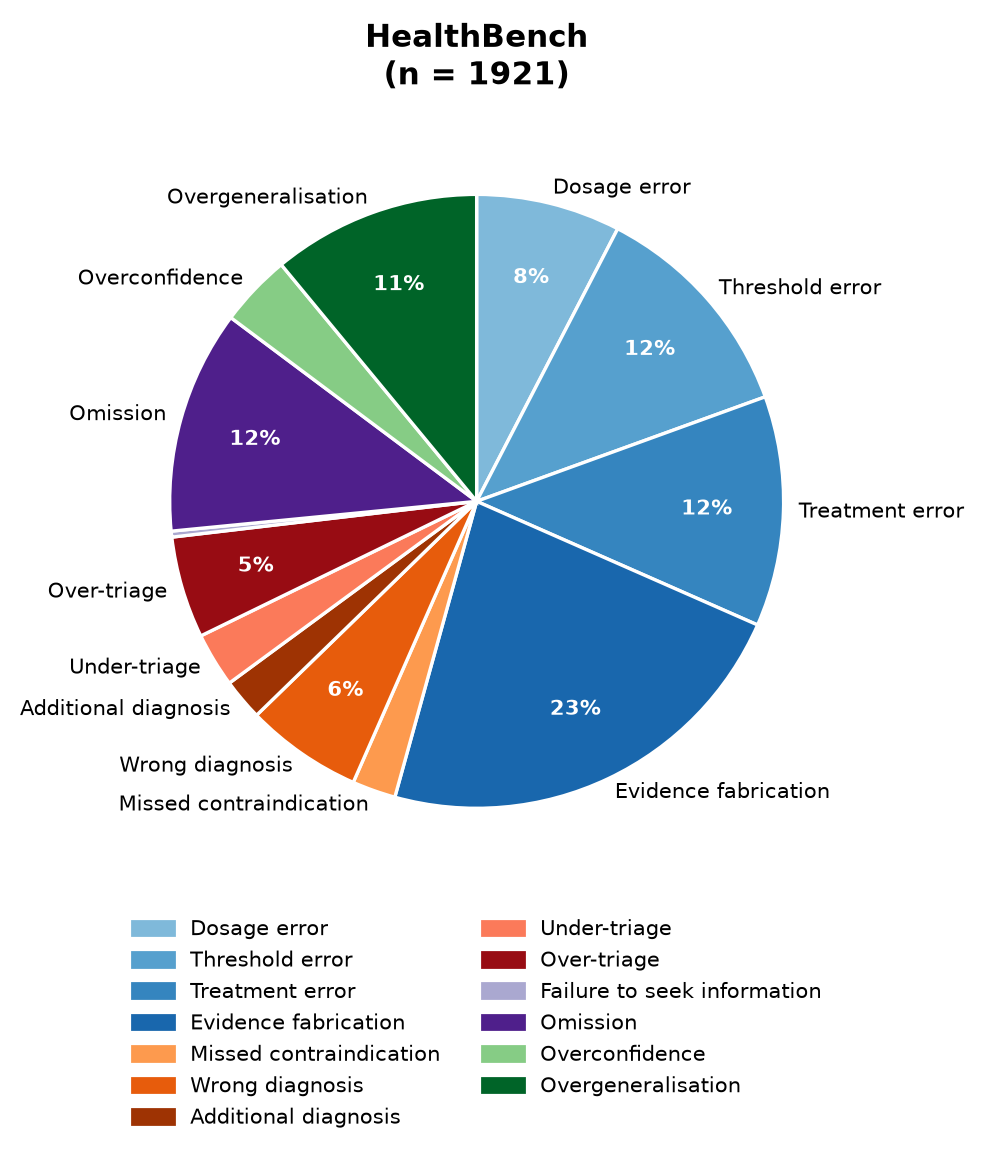
\includegraphics[width=0.65\columnwidth]{figures/error_taxonomy/injected_errors_healthbench.png}
\caption{Distribution of injected error types for HealthBench (n=1,921).}
\label{fig:err-dist-hb}
\end{figure}


\paragraph{HealthBench Professional.}
HealthBench Professional is a benchmark for evaluating LLM performance and safety on clinician-relevant professional tasks, designed to complement HealthBench's broader evaluation task \citep{hicks2026healthbench}. Whilst the main HealthBench set skews towards patient interactions \citep{arorahealthbench2025}, HealthBench Professional consists of 525 physician-authored tasks spanning three clinician-facing use cases: 
\begin{itemize}
    \item Care consult: reasoning through differentials, management and treatment.
    \item Writing and documentation: medical coding, note generation, patient messaging, summarisation and structured documentation.
    \item Finding and synthesising evidence relevant to clinical and scientific questions.
\end{itemize}

The 525-example set consists of real, heavily vetted clinical queries from 190 physicians across over 50 countries, each paired with a physician-written rubric. 
OpenAI grades this dataset internally with GPT-5.4 (at low reasoning effort) rather than the reference rubric-grader used for the original HealthBench. We preserve this difference for comparability with their reported results by using GPT-5.4 as a judge for Professional specifically, in place of the GPT-4.1 used for HealthBench proper and LiveMedBench. 11 of the 525 examples are straight refusals with nothing for a rubric to score. These were excluded before injection, leaving a usable answer set of 514 examples. Answers again come from openai/o3. A full taxonomy breakdown of the HealthBench Professional set is shown in Figure~\ref{fig:err-dist-hbpro}.

\begin{figure}[!h]
\centering
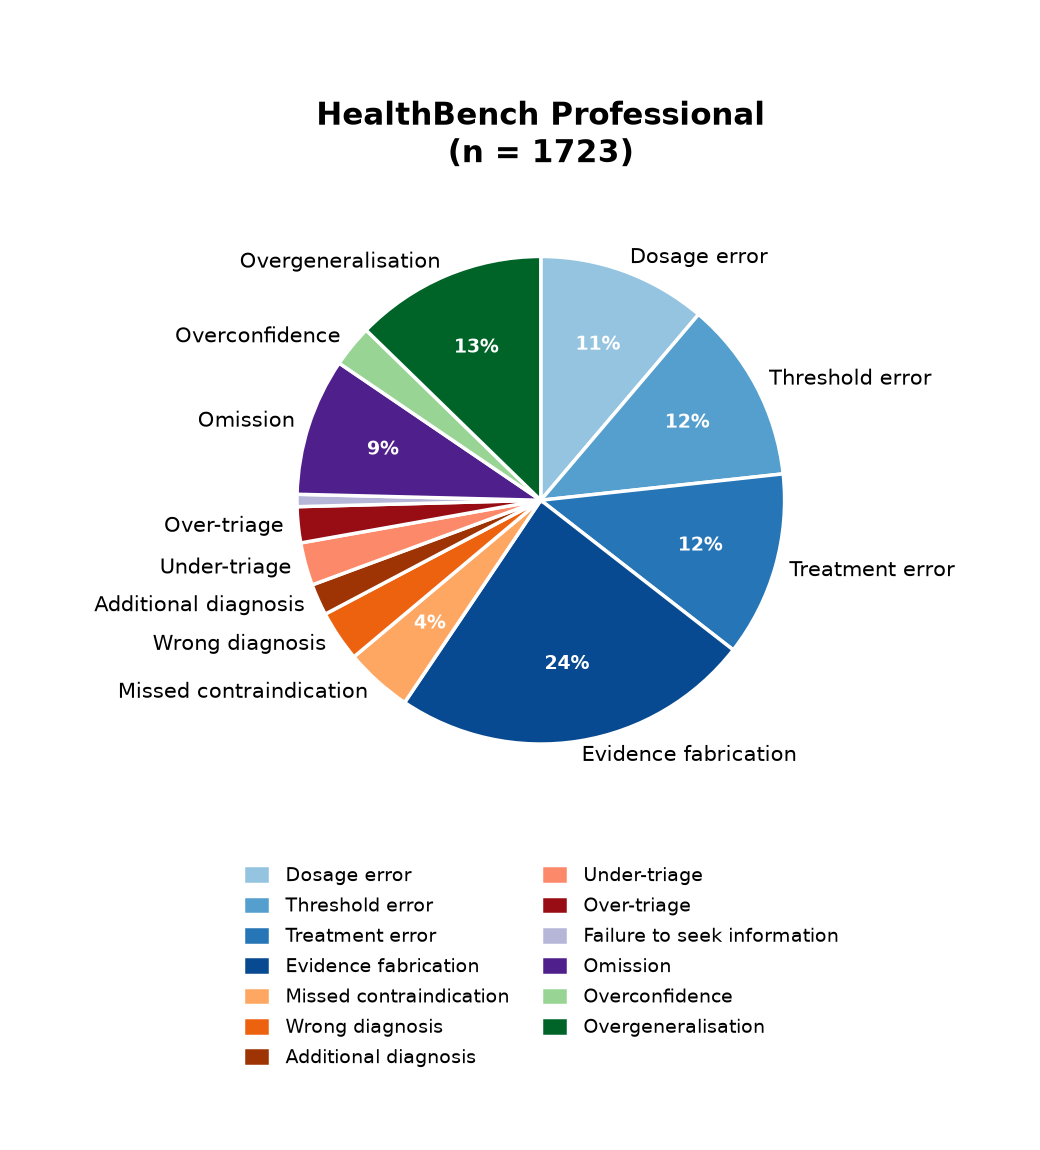
\includegraphics[width=0.85\columnwidth]{figures/error_taxonomy/injected_errors_healthbench_professional.png}
\caption{Distribution of injected error types for HealthBench Professional (n=1,723).}
\label{fig:err-dist-hbpro}
\end{figure}



\paragraph{LiveMedBench.}
LiveMedBench is a regularly updated medical question-answering rubric-based benchmark \citep{yan_livemedbench_2026}. LiveMedBench continuously harvests real-world online clinical cases, ensuring minimal contamination from model training data. 

We pin one snapshot by content hash (\texttt{v202604\_new.json}, SHA-256: \texttt{8b0fffad\ldots}) so every result reported here refers to one fixed case set regardless of later upstream changes. This snapshot corresponds to 5,286 cases, each with a patient narrative, core request and (where applicable) doctor advice, alongside a rubric of scored criteria whose items are tagged by clinical axis (axe) and by a case-level theme. A strict rule where any Chinese, Japanese, and Korean (CJK) character in the narrative, request or advice text marks a case as Chinese splits the snapshot into 2,666 English and 2,620 Chinese cases; we work from only the English half.

From this pool we draw a theme-balanced sample as opposed to a uniform random one: a target of 550 cases in equal quotas across five different themes (Context-Seeking, Emergency Referrals, Expertise-Tailored, Responding under Uncertainty, Response Depth), capped by the theme with the fewest available cases (Emergency Referrals, 84), with the shortfall redistributed across the rest. It is therefore pertinent to note that this inflates Emergency Referrals from 3.1$\%$ of the English pool to 15.3$\%$ of the sample - a deliberate oversample rather than the dataset's natural distribution. A 35-case top-up brings the total working set to 585 questions. From this 585 set, we found that 64 already score at or below the o3 baseline, thus leaving no headroom for an injected error to register as a further loss. We therefore exclude these 64 questions as a preprocessing step, resulting in 521 usable questions, of which 512 receive at least one accepted injection. A full taxonomy breakdown of the LiveMedBench set is shown in Figure~\ref{fig:err-dist-lmb}.

A summary of datasets and samples used in the main study pipeline is shown in Table~\ref{tab:dataset-summary}.

\begin{figure}[!h]
\centering
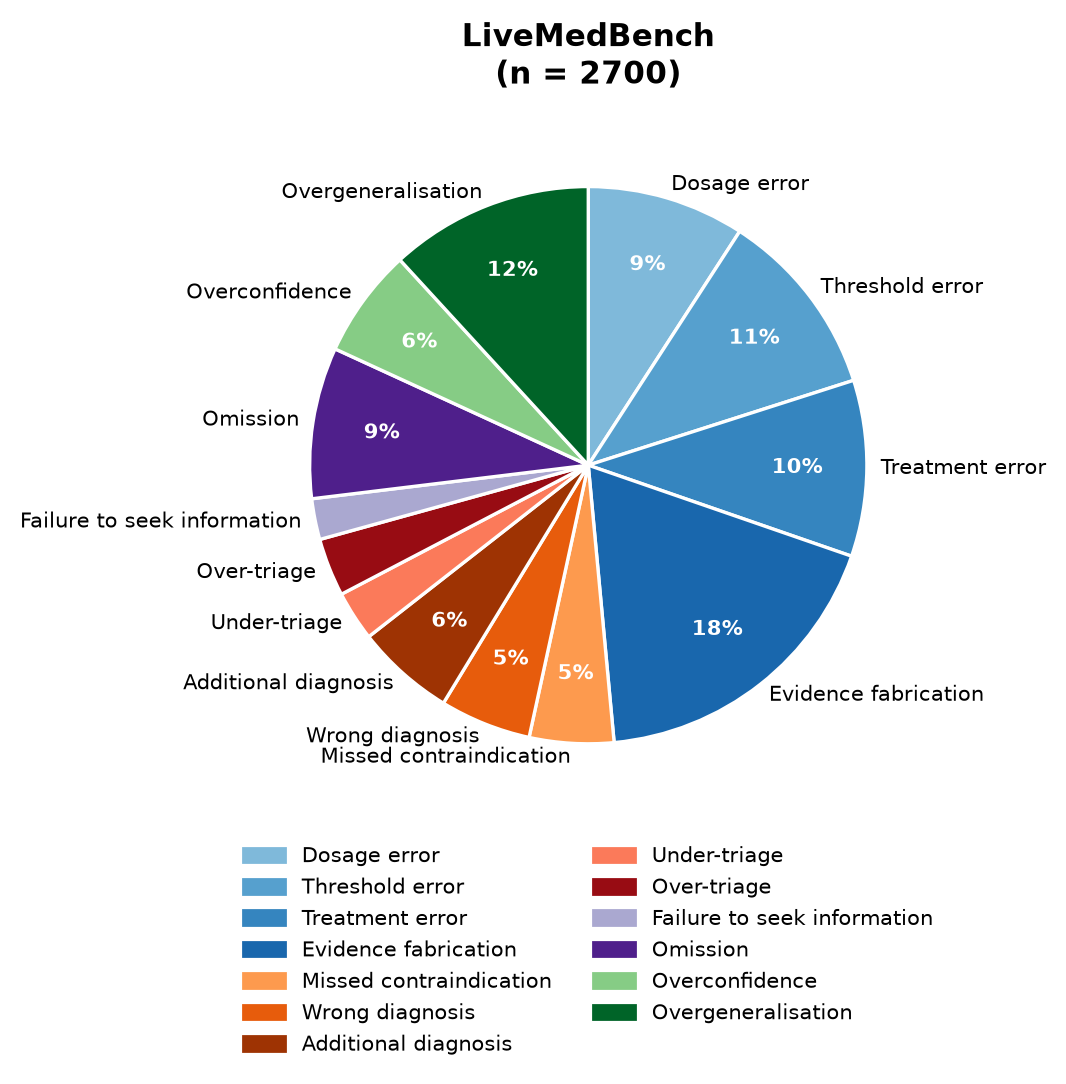
\includegraphics[width=0.85\columnwidth]{figures/error_taxonomy/injected_errors_livemedbench.png}
\caption{Distribution of injected error types for LiveMedBench (n=2,700).}
\label{fig:err-dist-lmb}
\end{figure}


\begin{table}[!h]
\centering
\small
\caption{Datasets and samples used throughout the study. See the
paragraphs above for how each pool was sampled and why some answers
were excluded. \textsuperscript{a} English-language half of the 5286-case snapshot (see LiveMedBench paragraph); the full theme-balanced draw and top-up together yield the 585 sampled.}
\label{tab:dataset-summary}
\begin{tabular}{@{}llrrrr@{}}
\toprule
Dataset & Sample & Pool & Sampled & Usable & Injected pairs \\
\midrule
HealthBench (main)       & fixed         & 5000 & 500 & 500 & 1921 \\
HealthBench Professional & full physician-authored set         & 525  & 525 & 514 & 1723 \\
LiveMedBench              & theme-balanced + top-up             & 2666\textsuperscript{a} & 585 & 521 & 2700 \\
\bottomrule
\end{tabular}
\vspace{2pt}
\end{table}


\newpage
\onecolumn
\appendixsection{Models Used: HealthBench Pipeline}
\label{appendix:models_used}
In this section, we report the different models used in our HealthBench/HealthBench Professional/LiveMedBench error-injection pipelines. Unless otherwise specified, all model runs use temperature set to 0 for reproducibility, default settings, and are called using API calls. Prompt caching was used to save computational cost, but was cleared after every experiment.

\subsection*{Error-Injection/Answer-Generation Models}
% We applied our HealthBench error injection pipeline to a range of models. This is shown in Figure \ref{fig:plus-design}, which shows the ``plus-shape'' design of the experiment for HealthBench.
% \begin{figure*}
% \centering
% \includegraphics[width=0.8\textwidth]{figures/plus_design.png}
% \caption{Figure showing the ``plus-shape'' design of our HealthBench experiment}
% \label{fig:plus-design}
% \end{figure*}
We varied two components: the answer-generation model and the error-injection model. We do this to test how robust our conclusions are across a range of answer-generation and error-injection model combinations. The answer-generation model is the model that generates the base answer that we then go on to alter with the error-injection pipeline. For our experiment, we used one of Kimi-K3 \citep{kimiteam2026kimik3}, o3 \citep{openai2025o3o4mini} and OpenBioLLM-70B \citep{pal2024openbiollms} as the base answer generation models. The error-injection model is the model that performs the ``injection'' phase where an error is added to the answer. For this, we used Gemini-3.1-Flash-Lite \citep{google2026gemini31flashlite}, DeepSeek-V3.2 \citep{deepseekai2025deepseekv32} and Qwen3.6-Flash \citep{qwenteam2026qwen36flash}. We experimented with Llama-3.3-70B as an error injection model, but found it unsuitable due to poor instruction following (Appendix \ref{appendix:llama}).

For HealthBench Professional and LiveMedBench, we only used o3/Gemini-3.1-Flash-Lite as answer-generation/error-injection respectively due to computational expense. Our analysis of the stability of our conclusions across different combinations of answer-generation and error-injection models (our analysis of stability across answer-generation and error-injection models in Appendix~\ref{appendix:healthbench_answer_injection_stability} supports this). All comparisons between HealthBench and these other datasets use the same model combination.

\subsection*{Grader Models}
For grader models, we used GPT-4.1 \citep{openai2025gpt41} for HealthBench and LiveMedBench. This is because HealthBench indicated that it had the best grader performance in their original work \citep{arorahealthbench2025}, and to be consistent with existing grader settings by their authors. We use UK AISI's implementation of HealthBench \citep{inspectevals}, as it decouples generation from grading, allowing error injection between the two stages, and supports batched grader calls. For consistency we use the same implementation for grading across all datasets. For HealthBench Professional, we use GPT-5.4 \citep{openai2026gpt54api} at low-reasoning to match the configuration in their original evaluation. All graders are called using API calls at temperature 0.

\subsection*{Applicability Models}
For the applicability check, we use a pair of models. For every single answer in the original, unperturbed dataset, each model independently assesses whether it meets each component of the error taxonomy. This check is carried out independently for every potential error-type, with custom checks for each. Unless the two models are unanimous in their agreement, that error type will not be judged applicable. The reasoning used by the applicability models is then given as context to the error-injection model. We use Gemini-3.7-Flash \citep{google2026gemini37flash} and GPT-5.6 Luna \citep{OpenAI2026GPT56} for this phase. 

\subsection*{Judge Models}
As part of our pipeline, we have an LLM judge model that is tasked with determining whether a particular error that was injected is valid. It checks whether the injected error was of the specified error-type from our taxonomy, that it could plausibly change the management/diagnosis of the patient (that is: the error is relevant) and that the error grammatically makes sense with the rest of the response. Though we previously criticised the instability of LLM judges, we give the judge a very controlled task, therefore likely reducing instability. It is required to give reasoning for all of its steps, and we spot-checked this reasoning thoroughly. We explored a few judges, but found GPT-5.6 Luna on ``Pro'' reasoning to be the best trade-off between accuracy and cost \citep{OpenAI2026GPT56}. We used this judge model for every experiment. We remark that between the programmatic checks and the clinician review, the judge model is further validated by other sections of our pipeline. Future work should explore the impact of using other judge models and whether this substantially changes the answer.

\subsection*{Summary}
A detailed summary of models used for answer generation, error-injection and grading for the HealthBench/HealthBench Professional/LiveMedBench experiments at each stage of the pipeline is shown in Table~\ref{tab:model-summary}. Every model slot in the pipeline runs with temperature 0, with batch API calls for grading. 

\begin{table}[H]
\centering
\small
\caption{Models used at each pipeline stage, across all three datasets, with
the resulting number of (correct, error-injected) pairs. Applicability
checking used Gemini-3.7-Flash and GPT-5.6 Luna Pro on
both sides (batched) throughout, and the injection-stage judge was
GPT-5.6 Luna Pro throughout; both are
constant across every row and omitted for space.}
\label{tab:model-summary}
\begin{threeparttable}
\begin{tabular}{@{}llllr@{}}
\toprule
Dataset & Answer model & Error-injection model & Grader & Pairs \\
\midrule
HealthBench (main)   & o3             & DeepSeek-V3.2         & GPT-4.1\tnote{b} & 2039 \\
                     & Kimi-K3        & DeepSeek-V3.2         & GPT-4.1 & 2022 \\
                     & OpenBioLLM-70B & DeepSeek-V3.2         & GPT-4.1 & 1665 \\
                     & o3             & Gemini-3.1-Flash-Lite & GPT-4.1\tnote{d} & 1921 \\
                     & o3             & Qwen3.6-Flash         & GPT-4.1 & 1780 \\
\addlinespace
HealthBench Prof.    & o3             & Gemini-3.1-Flash-Lite & GPT-5.4\tnote{a,c} & 1723 \\
\addlinespace
LiveMedBench         & o3             & Gemini-3.1-Flash-Lite & GPT-4.1 & 2700 \\
\bottomrule
\end{tabular}
\begin{tablenotes}[flushleft]\footnotesize
\item[a] Reasoning-effort set to low, matched to the o3 baseline's grading
  configuration for this dataset; every other grading run used the grader's
  default settings.
\item[b] OpenAI's own reference grader for HealthBench, hardcoded as
  GPT-4.1-2025-04-14 in the simple-evals implementation
  behind \citep{arorahealthbench2025}.
\item[c] Matches OpenAI's documented internal grading configuration for
  this dataset specifically \citep{hicks2026healthbench}.
\item[d] The only configuration feeding the headline cross-dataset
  result (Section~\ref{sec:hallucinations}). The
  o3/DeepSeek-V3.2 row is subsampled for fact-checking
  (Appendix~\ref{appendix:solution_breakdown}), and clinical review
  (Appendix~\ref{appendix:clinicalreview}) takes 39 pairs from each of the
  three o3 injector rows. Kimi-K3 and
  OpenBioLLM-70B feed no main-text result; with
  o3/DeepSeek-V3.2 they form the answer-model stability
  analysis (Appendix~\ref{appendix:healthbench_answer_injection_stability}),
  and Kimi-K3's acceptance rate is a comparison point in the
  Llama-3.3-70B-Instruct pilot (Appendix~\ref{appendix:llama}). The five
  configurations use 1,499 unique usable answers (500 o3, 499
  Kimi-K3, one failed to generate, 500 OpenBioLLM-70B)
  and yield 9,427 injected pairs.
\end{tablenotes}
\end{threeparttable}
\end{table}

\newpage
\onecolumn
\appendixsection{Clinical Review}\label{appendix:clinicalreview}

\paragraph{Clinical review setup.} To assess whether the accepted injections were actually meaningful, and not just trivial edits that happened to pass diff, span and length checks, a sample of accepted injections was independently reviewed by practising and training clinicians. 117 question and answer pairs were drawn from the o3 accepted injection set, stratified by error type and error-injection model (13 types $\times$ 3 injectors $\times$ 3 pairs per cell), hence the comparisons between injectors are not confounded with which questions each error-injector happened to alter. All question and answer pairs from the sample were in English. Each pair was assigned to two independent reviewers and presented as an original/edited comparison with the changed span of the answer highlighted, hence totalling to 234 reviews. For each pair, reviewers answered a single question: \textit{``Could it change the diagnosis or management of the patient?''}, with a required Yes/No answer box and an option to provide a reason to explain their decision. In total, there were 12 reviewers across a mixture of medical backgrounds (Figure~\ref{fig:panel_composition}). 11 of the reviewers reviewed 20 pairs each, with one reviewing 14 pairs in order to reach 234 reviews.

\paragraph{Overall agreement results.} 80.3$\%$ of the 234 reviews were ``Yes'' ([75.2\%, 85.5\%], cluster bootstrap over the 117 pairs, 10{,}000 resamples), i.e. the injected answer \textbf{does} change the patient's diagnosis or management. Raw pairwise agreement was 69.2\% (81/117 pairs).

\paragraph{Note on $\kappa$.} Cohen's $\kappa$ assumes the same two raters label every item, so each rater's individual ``Yes'' tendency can be estimated and used to define chance agreement. In this experiment, every pair is rated by a different pair of clinicians drawn from the 12-person panel, hence the raters are not fixed. Computing $\kappa$ requires an arbitrary per-item choice of which reviewer's answer is which. Recomputing per-type $\kappa$ under 200 random relabellings of that choice shows several types (F4, K1, K2, C3, O1) swing across zero, including flipping sign, from that arbitrary choice alone: the statistic reflects the labelling convention as much as any real agreement.

Fleiss' $\kappa$ avoids this issue, requiring only per-item agreement and the pooled ``Yes'' rate for 2 ratings/item. However, even for the best-powered 81-pair group (the nine "directly wrong" types below), $\kappa=0.29$ (95\% bootstrap CI $[-0.01,0.57]$), compared with 84.0\% raw agreement (95\% CI $[75.3\%,91.4\%]$). This instability reflects the skewed base rate (80\% Yes), which reduces $(1-p_e)$ and amplifies sampling noise in $\kappa$. We therefore report raw pairwise agreement as the more stable statistic for these data.

\paragraph{Two regimes.} Grouping the 13 error-types by edit mechanism reveals two distinct regimes. Nine types (C1, C2, F1, F2, F3, K2, O1, O2, R1) issue a directly wrong fact or instruction: a contraindicated drug, a wrong diagnosis, a wrong dose or threshold, an unsupported treatment claim, a dropped scope qualifier, an omitted workup or management step, or under-triage. Across these nine error-types (81 pairs, 162 ratings), reviewers agreed 84$\%$ of the time and rated 87.0$\%$ as diagnosis/management-changing (95$\%$ CI $[80.9\%, 92.6\%]$). The remaining four error-types (namely F4, K1, C3, R2) modify or extend claims without directly contradicting them (e.g. fabricated citations, added certainty or over-triage). Across these 36 pairs, the ``Yes'' rate fell to 65.3$\%$ (95$\%$ CI $[56.9\%, 73.6\%]$) and reviewer agreement also sharply fell to 36.1$\%$. Thus, the pooled results obscure substantial clinical disagreement over whether these subtler edits would change management, as opposed to simply being an artefact of measurement.

\begin{figure}[h]
    \centering
    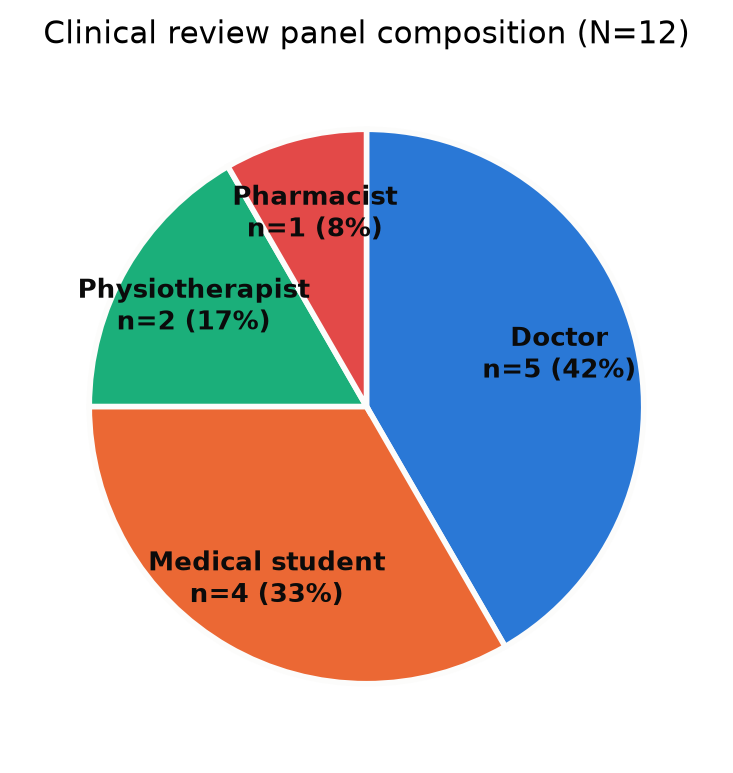
\includegraphics[width=0.5\textwidth]{figures/panel_comp.png}
    \caption{Composition of the 12-clinician review panel - five qualified doctors, 4 medical students, two senior physiotherapists and one clinical pharmacist.}
    \label{fig:panel_composition}
\end{figure}

\paragraph{Per-error-type breakdown.} Table~\ref{tab:clinical_review_by_type} gives, for each of the 13 error types: the `Yes' rate across both ratings, and raw pairwise agreement. It is prudent to note that with only nine pairs per type these are noisy individually, and thus Table~\ref{tab:clinical_review_by_type} should be considered alongside the two-regime grouping above and the worked examples provided below, rather than as precise per-type effect sizes.

\begin{table}[h]
\centering
\begin{tabular}{lrr}
\toprule
Error type & Yes \% & Agreement \% \\
\midrule
C1 & 94.4 & 88.9  \\
C2 & 77.8 & 77.8  \\
C3 & 72.2 & 44.4  \\
F1 & 100.0 & 100.0 \\
F2 & 100.0 & 100.0 \\
F3 & 94.4 & 88.9  \\
F4 & 50.0 & 22.2  \\
K1 & 66.7 & 33.3  \\
K2 & 66.7 & 55.6  \\
O1 & 55.6 & 55.6  \\
O2 & 94.4 & 88.9  \\
R1 & 100.0 & 100.0 \\
R2 & 72.2 & 44.4  \\
\bottomrule
\end{tabular}
\caption{Clinical review outcomes by error type (9 pairs, 18 ratings per type). Key: C1 = missed contraindication; C2 = wrong diagnosis; C3 = additional diagnosis; F1 = dosage error; F2 = threshold error; F3 = treatment error; F4 = evidence fabrication; K1 = overconfidence; K2 = overgeneralisation; O1 = failure to seek information; O2 = omission; R1 = under-triage; R2 = over-triage.}
\label{tab:clinical_review_by_type}
\end{table}


\paragraph{Per-injector breakdown.} Agreement and ``Yes'' rate are shown per error-injector model in Table~\ref{tab:clinical_review_by_injector}, with models showing broadly similar ``Yes'' rates across the board.


\begin{table}[h]
\centering
\begin{tabular}{lrrr}
\toprule
Injector model & $n$ pairs & Yes \% & Agreement \% \\
\midrule
DeepSeek-V3.2          & 39 & 75.6 & 71.8 \\
Gemini-3.1-Flash-Lite  & 39 & 79.5 & 59.0 \\
Qwen3.6-Flash          & 39 & 85.9 & 76.9 \\
\bottomrule
\end{tabular}
\caption{Clinical review outcomes by injector model (39 pairs per model).}
\label{tab:clinical_review_by_injector}
\end{table}

\begin{tcolorbox}[title=Worked example: clear agreement.]
\small
\label{Worked example:clear agreement.}
\paragraph{Pair drawn from C1 (contraindicated medication) injected by Qwen3.6-flash.} The question concerned a child's ear infection; the injected answer replaced ``pain/fever medicine (like acetaminophen or ibuprofen)'' with ``pain/fever medicine (like aspirin)''. Both assigned reviewers answered `Yes':

\begin{quote}
\small
\textit{Medical Student:} ``[...] given the clinical history and phrasing this case seems like a child under the age of 16 -- in which case they should not be given aspirin for pain relief due to the risk of Reye's syndrome. [...] Using the phrase `like aspirin' is also dangerous -- it is likely that doctors will have previously advised parents to use pain relief such as paracetamol or ibuprofen [...] but that could lead to parents therefore inferring from this that aspirin is safe to give to their child.''

\textit{Physiotherapist:} ``The example medication differs and suggesting `aspirin' can cause harm to the child if taken in some cases.''
\end{quote}
\end{tcolorbox}


Both reviewers, from different clinical backgrounds, independently converged on the same verdict and the same underlying reason (Reye's syndrome risk), despite one giving a much more detailed justification than the other.


\begin{tcolorbox}[title=Worked example: disagreement.]
\small
\label{Worked example:disagreement.}
\paragraph{Pair drawn from F4 (Evidence fabrication), injected by Qwen3.6-flash.} The question asked about the safety of hair transplant surgery; the injected answer attached an invented citation -- ``a 2023 International Society of Hair Restoration Surgery registry analysis of over 15,000 cases'' -- to a graft-survival statistic that was already stated correctly. The two assigned reviewers split:

\begin{quote}
\small
\textit{Physiotherapist (No):} ``Again, although unethical, it does not directly change the diagnosis or the management of the patient. It may encourage the patient to go ahead with treatment however the benefits/risks are already outlined thoroughly enough that it should help the patient make an informed decision regardless of the article stated.''

\textit{Doctor (Yes):} ``Patient may be more likely to accept/consent to a course of treatment founded on invented clinical evidence.''
\end{quote}
\end{tcolorbox}

Neither reviewer disputes that the citation is fabricated, or that the number it is attached to happens to be correct; they disagree on whether manufacturing false authority for an already-true claim changes what the patient goes on to do. This is the pattern behind most of the F4/K1/C3/R2 disagreements: the edit reframes or reinforces a claim rather than contradicting it, so the disagreement is about a harder second-order question: whether added (if unearned) confidence changes the patient's or clinician's downstream decision, not about a missed clinical fact.

\newpage
\onecolumn
\appendixsection{Fact-Checking Grader Results}
\label{appendix:solution_breakdown}
During our work, we observed that there were error-types that were structurally impossible for rubrics to identify. One of our hallucination types, \textit{evidence fabrication}, added information like artificial statistics or references to studies that were not real in order to support its argument. This has been documented as an issue before in medical literature \citep{gravel-mayoclinic-2023, bhattacharyya-cureus-2023}. Even though there are rubric criteria in HealthBench that specifically give an answer negative points if it cites falsified or fake information, we find that in every single case in our dataset, the grader passes the hallucinated answer even though it contains a fake citation. Manual spot-checking of the grader model reasoning traces indicated that the grader model did not believe the citations \textit{were} fake, as they looked reasonable. We argued that there is a large category of error-types that are not checkable within a rubric without external grounding. This includes spurious additional diagnoses and made up guidelines. To address this problem, we built a prototype fact-checking grader. This was a simplified implementation of the SAFE \citep{wei2024long-SAFE} pipeline from Google DeepMind. GPT-4.1 decomposes an answer into claims, converts each to a Google Search query via the Serper API \citep{serper}, and checks whether the results support it. The judge is the same model as our primary rubric grader; only the evidence available to it changes.

We applied this pipeline to 380 HealthBench pairs (correct answer, error-injected answer) across 11 error types (excluding omissions which remove claims that can then not be checked) and 3 error injection models. Each pair corresponds to a unique question from HealthBench. These pairs were selected so that the original grading gave them identical scores; that is, the rubric was unable to originally distinguish the correct and hallucinated answer results. Table \ref{tab:poc-results} shows the full results of this experiment.

\begin{table}[H]
\centering
\small
\begin{tabular}{
  @{}
  >{\raggedright\arraybackslash}p{\dimexpr 0.22\linewidth-2\tabcolsep\relax}
  >{\centering\arraybackslash}p{\dimexpr 0.06\linewidth-2\tabcolsep\relax}
  >{\centering\arraybackslash}p{\dimexpr 0.12\linewidth-2\tabcolsep\relax}
  >{\centering\arraybackslash}p{\dimexpr 0.20\linewidth-2\tabcolsep\relax}
  >{\centering\arraybackslash}p{\dimexpr 0.20\linewidth-2\tabcolsep\relax}
  >{\centering\arraybackslash}p{\dimexpr 0.20\linewidth-2\tabcolsep\relax}
  @{}
}
\toprule
Error Category & N & Claims per answer & Injected error identified as a claim & Error claim detected as unsupported & Original text detected as unsupported \\
\midrule
\addlinespace[2pt]
\multicolumn{6}{@{}l}{\textbf{Factual}} \\
Dosage error & 36 & 36.4 & 88.9 (74.7--95.6) & 93.8 (79.9--98.3) & \textit{55.6 (39.6--70.5)} \\
Threshold error & 36 & 36.5 & 83.3 (68.1--92.1) & 73.3 (55.6--85.8) & \textit{52.8 (37.0--68.0)} \\
Treatment error & 36 & 31.4 & 100.0 (90.4--100.0) & 97.2 (85.8--99.5) & \textit{61.1 (44.9--75.2)} \\
Evidence fabrication & 35 & 28.0 & 100.0 (90.1--100.0) & 100.0 (90.1--100.0) & \textit{54.3 (38.2--69.5)} \\
\addlinespace[2pt]
\multicolumn{6}{@{}l}{\textbf{Contextual}} \\
Missed contraindication & 29 & 32.0 & 93.1 (78.0--98.1) & 96.3 (81.7--99.3) & \textit{62.1 (44.0--77.3)} \\
Wrong diagnosis & 35 & 29.2 & 94.3 (81.4--98.4) & 84.8 (69.1--93.3) & \textit{40.0 (25.6--56.4)} \\
Additional diagnosis & 36 & 30.0 & 88.9 (74.7--95.6) & 90.6 (75.8--96.8) & \textit{61.1 (44.9--75.2)} \\
\addlinespace[2pt]
\multicolumn{6}{@{}l}{\textbf{Urgency}} \\
Under-triage & 29 & 27.3 & 93.1 (78.0--98.1) & 74.1 (55.3--86.8) & \textit{62.1 (44.0--77.3)} \\
Over-triage & 36 & 32.7 & \textit{63.9 (47.6--77.5)} & 87.0 (67.9--95.5) & \textit{52.8 (37.0--68.0)} \\
\addlinespace[2pt]
\multicolumn{6}{@{}l}{\textbf{Calibration}} \\
Overconfidence & 36 & 35.8 & 83.3 (68.1--92.1) & 83.3 (66.4--92.7) & \textit{44.4 (29.5--60.4)} \\
Overgeneralisation & 36 & 30.9 & 88.9 (74.7--95.6) & 78.1 (61.2--89.0) & \textit{63.9 (47.6--77.5)} \\
\midrule
Overall & 380 & 31.9 & 88.7 (85.1--91.5) & 87.5 (83.6--90.6) & 55.3 (50.2--60.2) \\
\bottomrule
\end{tabular}
\caption{Claim-level fact-checking of 380 pairs (error-injected and original answers) from distinct HealthBench questions, 29-36 per error type across the 11 non-omission types. The answers were generated by o3 across the three error-injection models: DeepSeek-V3.2, Gemini-3.1-Flash-Lite and Qwen3.6 Flash, and the factuality evaluator is \texttt{openai/gpt-4.1}. Pairs have tied and non-zero scores after HealthBench rubric evaluation. \textit{Original text detected as unsupported} is the same check on the original claim before the error injection. Figures are percentages with a 95\% confidence interval (Wilson).}
\label{tab:poc-results}
\end{table}

Given the low sample numbers, this should be treated as prototyping work rather than settled. However, we note that every error-type is identified as a claim significantly above chance. Where it is identified as a claim, every error-type is flagged as unsupported significantly above chance. This indicates that this is a potential solution to the structural problem that we argued with rubrics in Section~\ref{sec:clinical_taxonomy_analysis}.

\newpage
\onecolumn

\appendixsection{Programmatic Check}
\label{appendix:programmatic_check}
In the error injection pipeline, generated errors go through a programmatic check that they must pass before moving to the judge. We chose the thresholds by first tuning them against worked error examples in the prompts. Afterwards, we tested and tuned the thresholds by running the error injection pipeline and manually reviewing errors that passed or were rejected. As seen in Table \ref{tab:check-table}, the thresholds vary by each error type. For example, for the error type "Evidence fabrication", it is only allowed to increase the answer length up to 2 sentences, change up to 5 tokens from the original answer (Destroy 5), and touch at most 4 of the answer's sentences in making the edit read smoothly; it can also add an unlimited number of tokens. 

\begin{table}[H]
  \centering
  \small
  \setlength{\tabcolsep}{6pt}
  \begin{tabular}{@{}lllrrrc@{}}
    \toprule
    Type & Name & Diff shape & Destroy & Write & Sentences & Length \\
    \midrule
    \multicolumn{7}{@{}l}{\itshape Factual} \\
    \addlinespace[1pt]
    F1 & Dosage error & same & 6 & 6 & 4 & $-1$\,/\,$+1$ \\
    F2 & Threshold error & same & 6 & 6 & 4 & $-1$\,/\,$+1$ \\
    F3 & Treatment error & varied & 90 & 90 & 6 & $-1$\,/\,$+1$ \\
    F4 & Evidence fabrication & add.\ minor & 5 & $^{\dagger}$ & 4 & $0$\,/\,$+2$ \\
    \addlinespace[3pt]
    \multicolumn{7}{@{}l}{\itshape Contextual} \\
    \addlinespace[1pt]
    C1 & Missed contraindication & varied & 75 & 75 & 6 & $-2$\,/\,$+1$ \\
    C2 & Wrong diagnosis & varied & 75 & 74 & 3 & $-1$\,/\,$+1$ \\
    C3 & Additional diagnosis & additive & 0$^{\dagger}$ & $^{\dagger}$ & 1 & $0$\,/\,$+2$ \\
    \addlinespace[3pt]
    \multicolumn{7}{@{}l}{\itshape Urgency} \\
    \addlinespace[1pt]
    R1 & Under-triage & varied & 85 & 85 & 7 & $-1$\,/\,$+1$ \\
    R2 & Over-triage & varied & 85 & 85 & 7 & $-1$\,/\,$+1$ \\
    \addlinespace[3pt]
    \multicolumn{7}{@{}l}{\itshape Omission} \\
    \addlinespace[1pt]
    O1 & Failure to seek info & subtractive & $^{\dagger}$ & 3 & 6 & $-6$\,/\,$0$ \\
    O2 & Omission & subtractive & $^{\dagger}$ & 3 & 6 & $-6$\,/\,$0$ \\
    \addlinespace[3pt]
    \multicolumn{7}{@{}l}{\itshape Calibration} \\
    \addlinespace[1pt]
    K1 & Overconfidence & varied & 80 & 65 & 3 & $-2$\,/\,$+2$ \\
    K2 & Overgeneralisation & varied & 63 & 38 & 5 & $-1$\,/\,$+1$ \\
    \bottomrule
  \end{tabular}
  \caption{Per-type thresholds applied by the programmatic check.
    \textsc{destroy} refers to the number of tokens allowed to be deleted or edited in the original answer; \textsc{write} refers to the number of tokens that can be added. For some error types there are no limits and they are marked with $^{\dagger}$. \textsc{sentences}
    is how many of the answer's sentences the edit may touch, and \textsc{length} is the permitted net change in sentences; both are applied by taking one sentence to be 25 tokens.}
  \label{tab:check-table}
\end{table}



\newpage
\onecolumn 
\appendixsection{Compute Costs}\label{appendix:costs}

In this section we report the API costs of our experiments for each dataset (Table~\ref{tab:compute}).

\begin{table}[H]
\centering
\caption{Cost by pipeline stage and dataset, in USD.}
\label{tab:compute}
\begin{threeparttable}
\begin{tabular}{@{}lrrrr@{}}
\toprule
Stage & HealthBench & HealthBench Professional & LiveMedBench & Total \\
\midrule
Answer generation       & 17  & 3  & 5  & 25 \\
Applicability check & 45  & 12 & 14 & 71 \\
Error injection         & 225 & 52 & 40 & 317 \\
Grading                 & 255 & 32 & 60 & 347 \\
\midrule
Total                   & \$542 & \$99 & \$119 & \$760 \\
\bottomrule
\end{tabular}
\begin{tablenotes}[flushleft]\footnotesize
\item Answer generation used OpenAI and OpenRouter; applicability check and error injection used OpenRouter; grading used OpenAI throughout. Costs cover hosted API usage. Answer generation for OpenBioLLM-70B ran on institutional compute (2xH100) and incurred no billed API cost.
\end{tablenotes}
\end{threeparttable}
\end{table}

\newpage 
\onecolumn 
\appendixsection{MedHallu: Rubric Generation Models}
\label{appendix:rubric_generation_models}
We use a variety of methods to produce rubrics that we can evaluate, which we summarise in this section. A systematic evaluation of published rubric generation pipelines is beyond the scope of this work. Instead, we sample methods that construct rubrics at varying levels of generality. Generic rubric criteria are those that could be reasonably applied to virtually any example; specific rubric criteria are tailored for each example. We show an example below:

\begin{tcolorbox}[title=Example: specific vs general rubric criteria]
\small
\textbf{Question:} What is the cause of Type I diabetes? \\[4pt]
\textbf{Specific Rubric Criterion:} Does the answer identify that the cause of Type I diabetes is autoimmune attack of insulin-producing beta cells in the pancreas? \\[4pt]
\textbf{Generic Rubric Criterion:} Is the answer factually correct?
\end{tcolorbox}

\paragraph{Fully General Rubric.} We manually write a rubric that applies a fixed set of evaluation criteria to all questions. We design 12 rubric criteria, grouped into broader categories such as ``factual accuracy'', ``answer validity'' and ``limitation awareness''. This generic rubric is given in Appendix~\ref{appendix:generic-rubric}. This general rubric does not contain any specific medical facts, so acts as a baseline to understand the benefit of instance specific rubrics. These criteria were developed with reference to other generic rubric baselines used in the literature \citep{arorahealthbench2025, chen_automated_2026}. 

\paragraph{OpenRubrics.}\label{sec:openrubrics}
We use a rubric-generation model fine-tuned from Qwen3-8B, released as part of the OpenRubrics study \citep{liu2026openrubricsscalablesyntheticrubric} (details in Appendix~\ref{appendix:rubric_generation_models}). The model was trained via supervised fine-tuning on a corpus of (prompt, rubric) pairs constructed with the authors' ``contrastive rubric generation'' procedure, which derives rubrics by contrasting chosen and rejected responses to a prompt. We adopt this model for three reasons. Firstly, the full OpenRubrics corpus spans multiple domains, including medical. Secondly, at 8B parameters the model is inexpensive to run on limited academic compute. Thirdly, when used as the rubric-generation stage of a reward-modelling pipeline, it improved performance on HealthBench relative to baseline reward models, supporting its suitability for generating rubrics in the medical domain. Formally, for each example for which we want a rubric, we prompt the fine-tuned model $g_\theta$ to produce a rubric conditioned on that example's prompt. To remain faithful to how the model was trained, we use the same inference-time prompt template as the OpenRubrics authors. This template explicitly instructs the model to produce ``universal principles'' rather than topic-specific rubric items, which tends to make the generated rubrics fairly generic — though, since they are still conditioned on the prompt, less generic than a single fixed rubric applied uniformly across all examples. In our MedHallu study (Section~\ref{sec:medhallu}), this model produces 8.41 criteria on average (SD 1.05) per query.

\paragraph{RubricHub.} We use the pipeline designed in RubricHub \citep{li-etal-2026-rubrichub} to produce rubrics at the highest end of specificity, applying it as released without modification. In contrast to OpenRubrics, in this pipeline rubrics are generated conditioned on the query, a reference answer and some generic ``meta-principles'' such as clarity. The pipeline produces the rubric $\mathcal{R}_{final}$ for each query in three stages: (1) a reference response is generated. This reference response and the ``meta-principles'' are used to prompt an LLM to produce a per-model candidate rubric; (2) candidates from multiple frontier models are pooled and distilled into a single consensus rubric $\mathcal{R}_{base}$ via an aggregation prompt that removes redundancy and resolves conflicts; and (3) a difficulty-evolution step identifies a pair of consensus-high-scoring reference responses and prompts an LLM to extract additional criteria $\mathcal{R}_{add}$ that separate merely correct from exceptional responses, with $\mathcal{R}_{final} = \mathcal{R}_{base} \cup \mathcal{R}_{add}$. When using RubricHub to produce rubrics for our MedHallu experiment, we additionally provide the ``knowledge'' field of the dataset. This field corresponds to the ``body'' of the abstract that was used in generating the MedHallu/PubMedQA responses. RubricHub produced strictly more criteria than OpenRubrics on all 1000 paired MedHallu queries (mean 28.82 SD 4.01; Wilcoxon signed-rank test, $W=0$, $p < 0.001$). RubricHub also provides ``scores'' for each rubric criteria, with more important criteria given higher scores, unlike the other rubric generation methods we consider. The produced rubrics are also more specific, referring to named facts for each question. This is the explicit intention of the RubricHub pipeline, to reduce what the authors call ``rubric drift''. This allows us to evaluate whether specificity of rubric assists in detection of hallucinations. Additionally, the authors report state-of-the-art HealthBench performance when using the resulting rubrics for post-training, supporting the suitability of this pipeline for the medical domain specifically. We follow the authors' released prompt templates for all three stages without modification.

\newpage
\onecolumn
\appendixsection{Referential vs Self-Contained Responses in MedHallu}
\label{appendix:self-contained}
As discussed in the main text, many MedHallu \citep{pandit_medhallu_2025} responses are referential to the provided context, since correct answers often directly quote or summarise the source paper's results, which is an advantage hallucinated answers lack.

\begin{tcolorbox}[title=Example of a referential answer from MedHallu]
\small
\label{referential_example}
\textbf{Question:} Do mitochondria play a role in remodelling lace plant leaves during programmed cell death? \\[4pt]
\textbf{Correct Answer:} Results depicted mitochondrial dynamics in vivo as PCD progresses within the lace plant, and highlight the correlation of this organelle with other organelles during developmental PCD. To the best of our knowledge, this is the first report of mitochondria and chloroplasts moving on transvacuolar strands to form a ring structure surrounding the nucleus during developmental PCD. Also, for the first time, we have shown the feasibility for the use of CsA in a whole plant system. Overall, our findings implicate the mitochondria as playing a critical and early role in developmentally regulated PCD in the lace plant. \\[4pt]
\textbf{Hallucinated Answer:} Mitochondria regulate the formation of perforations in lace plant leaves through the modulation of calcium channels and by activating specific proteases that degrade cellular structure, facilitating the PCD process.
\end{tcolorbox}

We used a panel of three frontier-scale LLMs (Claude 4.8 Opus \citep{Anthropic2026Opus48}, Claude 5 Sonnet \citep{Anthropic2026Sonnet5}, GPT 5.6 Sol \citep{OpenAI2026GPT56}) to classify each correct answer as ``referential'', ``self-contained'', or ``borderline'' based on whether it made sense without the context field (prompt below). By majority vote, 510 answers were referential and 490 self-contained, with none borderline; 851 were unanimous across all three models (Fleiss' $\kappa=0.801$). Difficulty distribution did not differ significantly by label ($\chi^2$ test, $p=0.75$; Table~\ref{tab:contingency}).

\begin{table}[h!]
\centering
\begin{tabular}{lccc}
\hline
 & \textbf{Easy} & \textbf{Hard} & \textbf{Medium} \\
\hline
\textbf{Referential}      & 140 & 213 & 157 \\
\textbf{Self-contained}   & 134 & 195 & 161 \\
\hline
\end{tabular}
\caption{Contingency table of Difficulty by Majority Judgment}
\label{tab:contingency}
\end{table}

To test whether hallucinated answers are systematically less likely to be referential, we classified each hallucinated answer using the same scheme (Sonnet 5 only, as exploratory analysis). Table \ref{tab:hallu_vs_correct_answer} shows hallucinated answers are overwhelmingly self-contained regardless of the correct answer's classification (86.5\% when correct is referential, 99.2\% when correct is self-contained). This cements a structural advantage for referential correct answers, since they directly refer to evidence which is lacking for the hallucinated answer. 

\begin{table}[h!]
\centering
\begin{tabularx}{\textwidth}{l|XXX}
\toprule
 &
\textbf{Hallu. = Referential} &
\textbf{Hallu. = Self-contained} &
\textbf{Hallu. = Borderline} \\
\midrule
\textbf{Corr. = Referential} &
68 (13.3\%) &
441 (86.5\%) &
1 (0.2\%) \\
\textbf{Corr. = Self-contained} &
3 (0.6\%) &
486 (99.2\%) &
1 (0.2\%) \\
\bottomrule
\end{tabularx}
\caption{Distribution of hallucination classifications by correct answer classification. Percentages are calculated within each row.}
\label{tab:hallu_vs_correct_answer}
\end{table}

\begin{promptbox}[Referential/Self-Contained Classification Prompt]
\footnotesize
You will be given elements from a JSON dataset. Each element contains a \texttt{Question}, a \texttt{Knowledge} array (the source context), a \texttt{Ground Truth} answer, and an \texttt{AnswerCode}.

Your task is to classify the \texttt{Ground Truth} field only. Ignore the \texttt{Hallucinated Answer} field entirely.

\textbf{Criterion}

Judge whether the \texttt{Ground Truth} statement is self-contained: whether a reader who has never seen the \texttt{Knowledge} context could understand what claim is being asserted and, in principle, evaluate whether it is true.

Mark REFERENTIAL if any of the following hold: \\
$\bullet$~ It uses first-person or deictic reference to the source work (``our findings'', ``this study'', ``these results'', ``the present analysis'') \\
$\bullet$~ It contains a definite noun phrase whose referent appears only in the context (``the intervention'', ``the cohort'', ``the proposed model'') \\
 $\bullet$~ It reports a specific quantity, effect size, or comparison that is only meaningful relative to the described study (e.g.\ ``risk was reduced by $34\%$'' with no independently identifiable population or comparator) \\
 $\bullet$~ Its truth value depends on which specific study, cohort, dataset, or protocol is meant, such that the claim is neither true nor false in general

Mark SELF-CONTAINED if the statement expresses a general claim about the world that a domain expert could assess without the source document, even if that claim happens to have been derived from the study described in the context.

Mark BORDERLINE only if you genuinely cannot decide --- for example, a claim that is general in form but so narrowly scoped that its generality is doubtful.

\textbf{Note}: it is not sufficient for REFERENTIAL that the content of the answer is derivable from the context. That is true of every element in this dataset. The question is about linguistic and semantic dependence on the context, not about informational overlap.

\textbf{Examples} \\
     $\bullet$~ REFERENTIAL --- Ans\_0000: ``\ldots Overall, our findings implicate the mitochondria as playing a critical and early role in developmentally regulated PCD in the lace plant.'' Explicit first-person reference to the source work; ``our findings'' has no antecedent without the context. \\ 
     $\bullet$~ SELF-CONTAINED --- Ans\_0015: ``Opioid PCT is a feasible and acceptable therapeutic method to reduce refractory breathlessness in palliative care patients.'' A general clinical claim. An expert could assess it without seeing the study. \\
     $\bullet$~ REFERENTIAL (borderline case, resolved) --- ``Serum levels were significantly higher in the treatment group than in controls.'' No first-person marker, but ``the treatment group'' and ``controls'' have no referent outside the context, and ``serum levels'' of what is unspecified. Definite reference without antecedent is sufficient for REFERENTIAL even absent explicit study language. \\

\textbf{Output format}

Return a markdown table and nothing else --- no preamble, no summary, no commentary after the table. Exactly three columns:

\begin{center}
\texttt{| AnswerCode | Classification | Rationale |}
\end{center}

\texttt{Classification} must be exactly one of: REFERENTIAL, SELF-CONTAINED, BORDERLINE.

\texttt{Rationale} must be one sentence, under 20 words, naming the specific feature that drove the decision.

Judge each element independently. Do not let earlier classifications influence later ones.
\end{promptbox}

\newpage
\onecolumn
\appendixsection{Generic Rubric for MedHallu}
\label{appendix:generic-rubric}
As a baseline in our MedHallu experiment (see Section~\ref{sec:medhallu}), we wrote a generic rubric to be used for all questions. This was based on prior generic rubric baselines in the literature \citep{arorahealthbench2025, chen_automated_2026}. We have rubric criteria, each of which a response is independently measured against, grouped into broader dimensions like ``factual accuracy'' (Table~\ref{tab:evaluation_criteria}). We chose the number of criteria to be broadly similar to the number of rubric criteria produced by OpenRubrics.

\begin{table}[ht]
\centering
\small
\renewcommand{\arraystretch}{1.05}
\setlength{\tabcolsep}{4pt}
\begin{tabularx}{\textwidth}{|>{\raggedright\arraybackslash}p{0.26\textwidth}|X|}
\hline
\textbf{Dimension} & \textbf{Criterion} \\
\hline
Factual Accuracy &
$\bullet$~The response must be medically accurate and not contain factual errors.\par
$\bullet$~Where relevant and included, explanations should correctly refer to known biological or medical mechanisms or pathways.\par
$\bullet$~There should not be claims or statements that are not supported by medical literature or established scientific fact.
\\
\hline
Guideline/Practice Adherence &
$\bullet$~Where recommendations are made, they should align with the appropriate medical guidelines or codes of practice.\par
$\bullet$~Where the response makes a recommendation, and it is relevant to do so, it should name the specific medical guideline or code of practice that recommendation follows.
\\
\hline
Terminological Precision &
$\bullet$~The answer should use technical terms correctly, in their established sense.
\\
\hline
Unwarranted Specificity &
$\bullet$~The answer should not quote figures, data or named mechanisms at a level of specificity that is not required by the question or that is not supported by the evidence.
\\
\hline
Answer Validity &
$\bullet$~The response must be logically self-consistent and not contradictory.\par
$\bullet$~The response must make sense to whoever reads it.
\\
\hline
Answer Relevance &
$\bullet$~The response must be an appropriate and relevant answer to the original question.
\\
\hline
Completeness &
$\bullet$~The response should contain all of the information that is needed to respond to the question.
\\
\hline
Limitation Awareness &
$\bullet$~If the question is missing information that is needed, the response should identify this absence and request more information or highlight the gap in its own knowledge.
\\
\hline
\end{tabularx}
\caption{Evaluation dimensions and associated criteria.}
\label{tab:evaluation_criteria}
\end{table}

\newpage
\onecolumn
\appendixsection{Full MedHallu Results Breakdown}
\label{appendix:medhallu-breakdown}

Table~\ref{tab:combined_rubrics} reports MedHallu outcomes for every combination of rubric scheme, grader model and difficulty stratum. For each (correct, hallucinated) pair we record whether the rubric scored the correct answer higher, scored them equally, or scored the hallucinated answer higher; AUROC counts ties as $0.5$, so $0.5$ denotes chance.

\begin{table*}[!h]
\centering
\small
\setlength{\tabcolsep}{6pt}
\renewcommand{\arraystretch}{1.1}
\begin{tabular}{llccccl}
\toprule
& & \multicolumn{3}{c}{Pair outcome (\%)} & & \\
\cmidrule(lr){3-5}
Grader & Subset & Correct & Tie & Hallucinated & $p$ & AUROC [95\% CI] \\
\midrule
\multicolumn{7}{l}{\textit{Generic rubric}} \\
\addlinespace[1pt]
\multirow{4}{*}{Qwen3-14B}
 & Easy    & 67.9 & 15.7 & 16.4 & $<$0.001 & 0.757 [0.690, 0.821] \\
 & Medium  & 54.7 & 23.0 & 22.4 & $<$0.001 & 0.662 [0.596, 0.724] \\
 & Hard    & 26.2 & 27.2 & 46.7 & $<$0.001 & 0.397 [0.341, 0.456] \\
 & \textbf{Overall} & \textbf{46.9} & \textbf{22.7} & \textbf{30.4} & $<$0.001 & \textbf{0.583 [0.544, 0.621]} \\
\addlinespace[3pt]
\multirow{4}{*}{Llama3-70B}
 & Easy    & 64.2 & 26.1 &  9.7 & $<$0.001 & 0.772 [0.716, 0.828] \\
 & Medium  & 60.2 & 24.8 & 14.9 & $<$0.001 & 0.727 [0.668, 0.783] \\
 & Hard    & 33.8 & 32.3 & 33.8 & 0.76     & 0.500 [0.444, 0.556] \\
 & \textbf{Overall} & \textbf{50.8} & \textbf{28.2} & \textbf{21.0} & $<$0.001 & \textbf{0.649 [0.613, 0.683]} \\
\addlinespace[3pt]
\multirow{4}{*}{GPT-4.1}
 & Easy    & 88.1 & 10.4 &  1.5 & $<$0.001 & 0.933 [0.899, 0.963] \\
 & Medium  & 81.4 &  9.9 &  8.7 & $<$0.001 & 0.863 [0.814, 0.907] \\
 & Hard    & 51.3 & 25.6 & 23.1 & $<$0.001 & 0.641 [0.585, 0.697] \\
 & \textbf{Overall} & \textbf{71.2} & \textbf{16.3} & \textbf{12.4} & $<$0.001 & \textbf{0.794 [0.763, 0.825]} \\
\midrule
\multicolumn{7}{l}{\textit{OpenRubrics}} \\
\addlinespace[1pt]
\multirow{4}{*}{Qwen3-14B}
 & Easy    & 64.9 & 19.4 & 15.7 & $<$0.001 & 0.746 [0.679, 0.806] \\
 & Medium  & 55.3 & 21.7 & 23.0 & $<$0.001 & 0.662 [0.596, 0.724] \\
 & Hard    & 41.0 & 20.5 & 38.5 & 0.82     & 0.513 [0.451, 0.574] \\
 & \textbf{Overall} & \textbf{52.2} & \textbf{20.6} & \textbf{27.1} & $<$0.001 & \textbf{0.626 [0.588, 0.663]} \\
\addlinespace[3pt]
\multirow{4}{*}{Llama3-70B}
 & Easy    & 64.9 & 19.4 & 15.7 & $<$0.001 & 0.746 [0.679, 0.810] \\
 & Medium  & 53.4 & 28.6 & 18.0 & $<$0.001 & 0.677 [0.618, 0.736] \\
 & Hard    & 48.2 & 20.0 & 31.8 & 0.056    & 0.582 [0.521, 0.641] \\
 & \textbf{Overall} & \textbf{54.5} & \textbf{22.7} & \textbf{22.9} & $<$0.001 & \textbf{0.658 [0.622, 0.696]} \\
\addlinespace[3pt]
\multirow{4}{*}{GPT-4.1}
 & Easy    & 65.7 & 20.9 & 13.4 & $<$0.001 & 0.761 [0.698, 0.821] \\
 & Medium  & 59.0 & 22.4 & 18.6 & $<$0.001 & 0.702 [0.640, 0.761] \\
 & Hard    & 44.1 & 27.7 & 28.2 & 0.10     & 0.580 [0.523, 0.639] \\
 & \textbf{Overall} & \textbf{54.9} & \textbf{24.1} & \textbf{21.0} & $<$0.001 & \textbf{0.669 [0.634, 0.705]} \\
\midrule
\multicolumn{7}{l}{\textit{RubricHub}} \\
\addlinespace[1pt]
\multirow{4}{*}{Qwen3-14B}
 & Easy    & 86.6 &  7.5 &  6.0 & $<$0.001 & 0.903 [0.858, 0.944] \\
 & Medium  & 69.6 &  9.9 & 20.5 & $<$0.001 & 0.745 [0.683, 0.808] \\
 & Hard    & 70.8 &  5.6 & 23.6 & $<$0.001 & 0.736 [0.677, 0.795] \\
 & \textbf{Overall} & \textbf{74.7} & \textbf{7.6} & \textbf{17.8} & $<$0.001 & \textbf{0.785 [0.750, 0.818]} \\
\addlinespace[3pt]
\multirow{4}{*}{Llama3-70B}
 & Easy    & 86.6 &  4.5 &  9.0 & $<$0.001 & 0.888 [0.836, 0.937] \\
 & Medium  & 77.6 &  8.7 & 13.7 & $<$0.001 & 0.820 [0.764, 0.873] \\
 & Hard    & 71.8 &  9.7 & 18.5 & $<$0.001 & 0.767 [0.710, 0.821] \\
 & \textbf{Overall} & \textbf{77.8} & \textbf{8.0} & \textbf{14.3} & $<$0.001 & \textbf{0.817 [0.784, 0.849]} \\
\addlinespace[3pt]
\multirow{4}{*}{GPT-4.1}
 & Easy    & 87.3 &  6.7 &  6.0 & $<$0.001 & 0.907 [0.862, 0.948] \\
 & Medium  & 73.9 & 11.8 & 14.3 & $<$0.001 & 0.798 [0.739, 0.851] \\
 & Hard    & 77.4 &  3.6 & 19.0 & $<$0.001 & 0.792 [0.736, 0.846] \\
 & \textbf{Overall} & \textbf{79.0} & \textbf{7.1} & \textbf{13.9} & $<$0.001 & \textbf{0.826 [0.793, 0.856]} \\
\bottomrule
\end{tabular}
\caption{\textbf{MedHallu results by rubric scheme, grader model and difficulty.}
\emph{Correct} / \emph{Tie} / \emph{Hallucinated} give the percentage of pairs in which the rubric scored the correct answer higher, scored both equally, or scored the hallucinated answer higher (rows sum to 100\%).
$p$ is from a Wilcoxon signed-rank test on the paired scores.
AUROC treats ties as $0.5$, with a percentile bootstrap 95\% CI; $0.5$ is chance.
Sample sizes are fixed across all cells: Easy $n=134$, Medium $n=161$, Hard $n=195$, Overall $n=490$.}
\label{tab:combined_rubrics}
\end{table*}

Figures~\ref{fig:win/tie/lossgeneric},~\ref{fig:win/tie/lossopen} and~\ref{fig:win/tie/lossrubrichub} show the broken down win/tie/loss rates per-grader model and per-hallucination difficulty, for each of the rubric schemes. These correspond to the correct $>$ hallucinated, tie and hallucinated $>$ correct columns in Table~\ref{tab:combined_rubrics}.

\begin{figure*}[!h]
\centering 
\includegraphics[width=0.8\linewidth]{figures/medhallu/Generic_Rubrics_Results.png}
\caption{Win/Tie/Loss rate breakdown per-hallucination and per-grader model using the generic rubric.}
\label{fig:win/tie/lossgeneric}
\end{figure*}

\begin{figure*}[!h]
\centering 
\includegraphics[width=0.8\linewidth]{figures/medhallu/openrubrics_breakdown.png}
\caption{Win/Tie/Loss rate breakdown per-hallucination and per-grader model using OpenRubrics generated rubrics.}
\label{fig:win/tie/lossopen}
\end{figure*}

\begin{figure*}[!h]
\centering 
\includegraphics[width=0.8\linewidth]{figures/medhallu/rubrichub_breakdown.png}
\caption{Win/Tie/Loss rate breakdown per-hallucination and per-grader model using RubricHub generated rubrics.}
\label{fig:win/tie/lossrubrichub}
\end{figure*}



\newpage
\onecolumn
\appendixsection{Fact-Checking Criteria in MedHallu}
\label{appendix:rubrichub-rubric-analysis}
\subsection*{Generic Rubric}
We had a hypothesis that it was primarily the fact-checking rubric criteria that were driving the discrimination between the correct and hallucinated answers during our MedHallu experiment. We tested this using our generic rubric (text in Appendix~\ref{appendix:generic-rubric}). One of the dimensions of our generic rubric was ``Factual Accuracy''. This was split into 3 criteria that asked the grader to determine different ways that a model response must be factually accurate. 

To test our hypothesis, we compared the gap between correct and hallucinated scores ($Gap = S(a_i^+) - S(a_i^-)$), broken down by the dimensions of the generic rubric. We did this check for GPT-4.1, since it was the strongest grader in MedHallu, but found qualitatively similar results for the other graders too. Figure \ref{fig:generic-rubric-breakdown} shows the breakdown of gap by dimension.
\begin{figure}[h!]
    \centering
    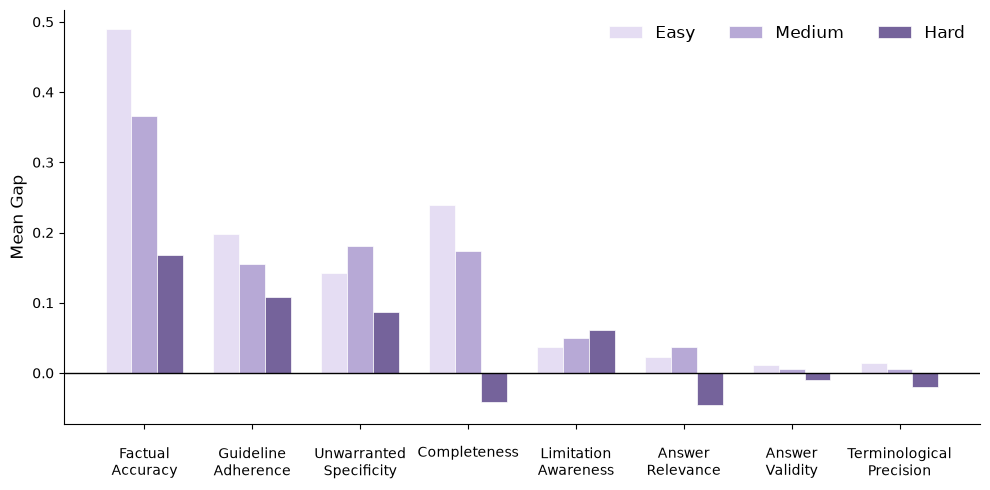
\includegraphics[width=0.8\linewidth]{figures/medhallu/generic-rubric-score-breakdown-gpt.png}
\caption{\textbf{Generic rubrics rely on the grader's factual knowledge to distinguish hallucinations.} For GPT-4.1, factual accuracy provides most of the separation between correct and hallucinated responses. Gap = Correct Score - Hallucinated Score}
\label{fig:generic-rubric-breakdown}
\end{figure}

Figure~\ref{fig:generic-rubric-breakdown} shows that, under the generic rubric, discrimination is concentrated in criteria requiring medical knowledge, such as factual accuracy and guideline adherence, while general criteria such as relevance, validity, and completeness provide little separation. For hard hallucinations, the hallucinated answers are assigned higher scores in these axes as they tend to be confidently wrong. This indicates that it is primarily factual criteria that distinguish between correct and hallucinated responses, and stylistic criteria are not effective for this.

\subsection*{RubricHub}
We had a hypothesis that the rubrics produced by RubricHub were highly factually specific, and that it was these specific facts that were driving the discrimination between correct and hallucinated responses that we showed in Section~\ref{sec:medhallu}. In order to assess this, we performed an experiment to classify the RubricHub rubric criteria into either \texttt{FACTCHECK} criteria, which check the presence in the response of a specific verifiable fact, or \texttt{OTHER} criteria, which check more general qualities like the answer confidence or tone. 

We used the rubrics that were generated for MedHallu questions where the correct response was ``self-contained'' and the hallucinated response was ``hard''. This is a subset of $195/1000$ MedHallu questions, yielding $5633$ unique rubric criteria. We used 3 LLMs (Grok-4.3 \citep{xAI2026Grok43}, Gemini-2.5-Flash \citep{Google2025Gemini25Flash}, GPT-5.6 Luna \citep{OpenAI2026GPT56}) to classify a randomly selected subset of $1000$ of these criteria into \texttt{FACTCHECK} or \texttt{OTHER}. We also included a \texttt{BORDERLINE} category for where models were not sure (prompt below). Each criterion was assessed independently, in batches of 100 per API call. 

We found that classifications for 79\% of the 1000 criteria were unanimous (Fleiss' $\kappa=0.68$). No criterion was classified as \texttt{BORDERLINE} by any model. To verify this was not an artifact of model capability, a similar analysis on a different random subset of $1000$ criteria with 3 stronger models (GPT-5.6 Terra \citep{OpenAI2026GPT56}, Claude-5-Sonnet \citep{Anthropic2026Sonnet5}, Muse-Spark-1.2 \citep{Meta2026MuseSpark12}) produced a $\kappa = 0.65$ and unanimous fraction $76\%$. Manual review of the non-unanimous cases indicated they were genuinely ambiguous examples.

Using these classification labels, we then used the scores for the rubric criteria that were measured by the GPT-4.1 grader in Section~\ref{sec:medhallu}. Since all of the grader models were consistent with each other, we expect the conclusions to be qualitatively true for the other graders as well. Given the classification labels, we measured two things:
\begin{enumerate}
    \item For the criteria that are \texttt{FACTCHECK}, are they significantly more likely (compared to \texttt{OTHER} criteria) to have neither response (correct or hallucinated) satisfy the criteria?
    \item For the criteria that are \texttt{FACTCHECK}, are they significantly more likely (compared to \texttt{OTHER} criteria) to discriminate between the correct and hallucinated responses (correct meets criteria and hallucinated does not), conditional on at least one response meeting the criteria?
\end{enumerate}
On only the unanimous cases, we found for 1. that \texttt{FACTCHECK} criteria are $1.35\times$ more likely than \texttt{OTHER} to have neither response meet the criteria (95\% confidence interval: $1.19$ -- $1.54$). For 2., we found that \texttt{FACTCHECK} criteria are $2.70\times$ more likely to discriminate than \texttt{OTHER} criteria (95\% confidence interval: $1.95$ -- $3.74$). If we include all $1000$ examples, we find instead $1.25\times$ for 1. ($1.13$ -- $1.38$) and $2.02\times$ ($1.59$ -- $2.57$) for 2. Given the high inter-model agreement ($\kappa = 0.65 - 0.68$) and robustness of downstream results to including the non-consensus classifications, we proceeded to classify all $5633$ criteria using GPT-5.6 Luna alone.

Table~\ref{tab:classification_patterns} shows the contingency table showing how Luna classified each criterion, and whether it discriminated or not between correct and hallucinated answers. Overall, 4431 (79\%) of answers were \texttt{FACTCHECK} and 1202 (21\%) were \texttt{OTHER}.
\begin{table}[!h]
\centering
\begin{tabular}{lcccc}
\toprule
\textbf{Classification} & \textbf{Discriminates} & \textbf{Both met} & \textbf{Both not met} & \textbf{Reversed} \\
\midrule
FACTCHECK  & 18.5\% & 8.4\%  & 73.1\% & 0.0\% \\
OTHER      & 15.0\% & 31.5\% & 53.5\% & 0.0\% \\
\bottomrule
\end{tabular}
\caption{Contingency table showing how the criteria discriminate between correct and hallucinated responses, depending on the classification by GPT-5.6 Luna. ``Discriminates'' gives the fraction of criteria where the correct answer met the criteria but the hallucinated did not. ``Reversed'' is the fraction where the hallucinated answer met the criteria, but the correct did not.}
\label{tab:classification_patterns}
\end{table}
We found that on all $5633$ criteria, \texttt{FACTCHECK} criteria were $1.37\times$ as likely as \texttt{OTHER} criteria to not be met by either response (95\% CI: $1.29$ -- $1.45$). Also, \texttt{FACTCHECK} criteria were $2.14\times$ as likely as \texttt{OTHER} criteria to distinguish between correct and hallucinated responses (95\% CI: $1.88$ -- $2.43$). These results are consistent with those from the subset of $1000$ criteria.

\subsection*{Impact on classification results}
We explored what happened to the classification performance on the subset of answers, if we were to exclude the \texttt{FACTCHECK} criteria from the rubrics produced by RubricHub. The results of this are shown in Table~\ref{tab:factcheck-criteria-excluded}.

\begin{table}[H]
  \centering
 \begin{tabularx}{\textwidth}{@{} l *{4}{>{\centering\arraybackslash}X} @{}}
    \toprule
    Subset & Win & Tie & Loss & AUROC \\
    \midrule
    Before (all criteria)
      & \makecell{0.774 \\ \scriptsize{[0.713, 0.831]}}
      & \makecell{0.036 \\ \scriptsize{[0.010, 0.062]}}
      & \makecell{0.190 \\ \scriptsize{[0.138, 0.246]}}
      & \makecell{0.792 \\ \scriptsize{[0.736, 0.846]}} \\[0.4em]
    After (FACTCHECK excluded)
      & \makecell{0.467 \\ \scriptsize{[0.400, 0.533]}}
      & \makecell{0.390 \\ \scriptsize{[0.323, 0.462]}}
      & \makecell{0.144 \\ \scriptsize{[0.097, 0.195]}}
      & \makecell{0.662 \\ \scriptsize{[0.610, 0.710]}} \\
    \bottomrule
  \end{tabularx}
    \caption{Win/tie/loss rates and paired AUROC before and after excluding
        FACTCHECK criteria from \texttt{fixed} (n=195 questions, 95\%
        bootstrap CIs).}
  \label{tab:factcheck-criteria-excluded}
\end{table}

The AUROC value is significantly lower (paired bootstrap on the AUROC values gives mean $-0.131$, 95\% CI: $-0.187 \rightarrow -0.077$). At the same time, the win rate falls significantly and the tie rate increases significantly. The loss rate does not significantly change. We conclude that it is the fact-checking criteria that disproportionately lead to discrimination between correct and hallucinated answers, and without them, the values are dominated by ties.

\begin{promptbox}[\texttt{FACTCHECK}/\texttt{OTHER} Prompt]
\footnotesize
You are a medical rubric classification expert. You will receive a list of rubric criteria --- each specifying a quality that an answer to a medical question should or should not possess --- and classify each criterion.

\textbf{Classification labels}

$\bullet$~ \textbf{FACTCHECK} --- A textbook or reference source alone would be sufficient to judge whether an answer satisfies this criterion. The criterion pins down a specific claim that is either right or wrong. \\

$\bullet$~ \textbf{OTHER} --- Judging this criterion requires editorial discretion: assessing tone, structure, completeness, clarity, emphasis, or coverage of a topic area. No single lookup could settle it. \\

$\bullet$~ \textbf{BORDERLINE} --- You cannot confidently determine which of the above applies.

\textbf{Decision test}

For each criterion, ask:

\begin{center}
``Could I judge whether an answer meets this criterion by looking something up in a reference source?''
\end{center}

$\bullet$~ \textbf{Yes} $\rightarrow$ FACTCHECK \\
$\bullet$~ \textbf{No, it requires judgement} $\rightarrow$ OTHER \\
$\bullet$~ \textbf{Genuinely unclear} $\rightarrow$ BORDERLINE

\textbf{Examples}

$\bullet$~ \textbf{FACTCHECK} --- Criterion: ``The answer should state that the cause of Type-I diabetes is autoimmune destruction of insulin-producing beta cells in the pancreas.'' \\
Rationale: One lookup confirms whether this mechanism is correct. \\

$\bullet$~ \textbf{OTHER} --- Criterion: ``The answer should use appropriate terminology correctly and in its proper context, such as `insulin' and `pancreas'.'' \\
Rationale: ``Appropriate use'' requires editorial judgement, not a single lookup. \\

$\bullet$~ \textbf{OTHER} --- Criterion: ``The answer should be well-structured with a heading, a body, and a concluding sentence.'' \\
Rationale: Structural formatting --- no factual reference needed. \\

$\bullet$~ \textbf{FACTCHECK} --- Criterion: ``States that reported cases involve young infants (approximately 2--15 months of age) with episodes specifically triggered by water immersion during bathing.'' \\
Rationale: Age range and trigger are concrete claims checkable against the literature. \\

$\bullet$~ \textbf{OTHER} --- Criterion: ``The answer should discuss the role of insulin in glucose metabolism.'' \\
Rationale: Names a topic area --- many different facts could satisfy it, and judging adequate ``discussion'' requires editorial discretion. \\

$\bullet$~ \textbf{FACTCHECK} --- Criterion: ``Explicitly states that syncope-like episodes during infant bathing are considered a proposed pediatric variant of water-induced urticaria, using hedged language (e.g.\ `may represent') rather than asserting certainty.'' \\
Rationale: The core claim is verifiable; the hedging requirement is secondary.

\textbf{Input format}

You will receive a JSON array of dictionaries, each with:
\begin{itemize}
    \item \texttt{criterion}: the text of the criterion
    \item \texttt{criterion\_code}: a unique identifier
\end{itemize}

Classify \textbf{every} criterion independently.

Do \textbf{not}:
\begin{itemize}
    \item omit, merge, reorder, or duplicate criteria
    \item allow earlier classifications to influence later ones
    \item attempt to maintain any particular balance or distribution of labels
\end{itemize}

\textbf{Output format}

Return the classification for every criterion, preserving the input order.
\end{promptbox}

\newpage 
\onecolumn
\appendixsection{MedHallu Context Leakage Result}
\label{appendix:medhallu-context-leakage}
As discussed in Appendix~\ref{appendix:rubric_generation_models}, RubricHub generated rubrics for our MedHallu problem that were significantly more detailed than the rubrics produced by OpenRubrics (mean $28.82$ rubric criteria per question for RubricHub vs $8.41$/question for OpenRubrics). Manual review of the rubrics also showed that the RubricHub rubrics were far more specific, spelling out particular facts that the answer should contain. This is a consequence of both rubric generation models. OpenRubrics explicitly encourages the creation of rubrics that are ``universal principles'' \citep{liu2026openrubricsscalablesyntheticrubric}, whereas RubricHub is concerned that these rubrics are too vague and lead to what the authors in that paper call ``rubric drift'' \citep{li-etal-2026-rubrichub}. 

When producing the rubrics for RubricHub, the rubric generation process was allowed to use the ``knowledge'' field in the MedHallu questions for additional information when generating the rubric for each question. This field originates in the way that the MedHallu questions were generated from PubMedQA answers. PubMedQA questions are research paper titles, reformatted into valid questions. The ``answer'' is the conclusion of the abstract. The ``knowledge'' is the remainder of the abstract, broken down into individual sentences. In providing the ``knowledge'' to RubricHub, our intention was to allow it to create much more specific rubrics in addition to its parametric knowledge that it may have. However, it raises the question of whether the knowledge contained in this field may indirectly answer this question.

Since each MedHallu question contributes exactly one correct and one hallucinated answer, we treat each question as a paired classification instance. We compute the paired AUROC---the proportion of pairs in which the correct answer receives a strictly higher rubric score than the hallucinated answer, with ties contributing 0.5. This directly measures the probability that rubric scores rank the correct answer above the hallucinated one within a given pair, without pooling across questions. Figure~\ref{fig:medhallu-rubrichub-auroc} reports the resulting AUROC values together with 95\% confidence intervals estimated by bootstrap resampling at the question level.

\begin{figure}[H]
    \centering
    \includegraphics[width=\linewidth]{figures/medhallu/medhallu_rubrichub_auroc.png}
    \caption{AUROC for hallucination discrimination on the MedHallu hard subset using RubricHub rubric scores, compared against a DeBERTa-v3-large NLI entailment baseline (orange). Error bars denote 95\% confidence intervals estimated by bootstrap resampling.}
    \label{fig:medhallu-rubrichub-auroc}
\end{figure}

To better understand this limitation, we compared RubricHub against a pretrained DeBERTa-v3-large natural language inference (NLI) cross-encoder. For each question, we paired the provided ``Knowledge'' field with both the correct and hallucinated responses and computed a support score as the difference between the model's entailment and contradiction probabilities. These scores were then used as classifier scores to compute an AUROC in the same manner as the rubric scores. The resulting AUROC values are shown in Figure~\ref{fig:medhallu-rubrichub-auroc} (orange). The entailment baseline overlaps the 95\% confidence interval of the RubricHub results, indicating that RubricHub provides only a modest improvement over a simple NLI-based factual consistency check.

This result suggests that the gains from highly specific rubrics arise primarily because the MedHallu context leaks much of the information needed to distinguish correct and hallucinated answers. Since the rubric generation pipeline derives its criteria directly from this context, rubric evaluation largely reduces to checking whether an answer is supported by the provided knowledge. In this case, where the context provides highly relevant information to the question, we see that rubric-based evaluation is only slightly outperforming a pure NLI-based check. In other words, MedHallu is an unusually friendly benchmark on which to evaluate rubric performance, because MedHallu answers and their accompanying knowledge context are both drawn from the same PubMedQA abstract. More realistic datasets that do not have access to such relevant context would likely see worse rubric performance.

\newpage
\onecolumn
\appendixsection{Llama-3.3-70B-Instruct Experiments}\label{appendix:llama}


Before settling on DeepSeek-V3.2, Qwen3.6-Flash and Gemini-3.1-Flash-Lite as error-injection models, Llama-3.3-70B-Instruct was also piloted as an error-injection model, judged throughout by GPT-5.6 Luna Pro. Three different serving configurations were tried (OpenRouter's hosted API, a local vLLM server, and direct HuggingFace Inference) across a number of small pilots and two full-scale attempts (Table~\ref{tab:llama-injector-pilots}). Error-acceptance rates were extremely low throughout. The two full scale attempts yielded acceptance rates of just 28.1\% (746/2656) and 41.6\% (162/389) on Kimi-K3 and o3 answers respectively - well below the 73.7\% acceptance rate that DeepSeek-V3.2 achieved on that identical question pool.

The vast majority of these failures were programmatic-check rejections, rather than applicability or judge rejections: combining the diff-shape and span checks accounts for 82.1\% (1569/1910) and 87.7\% (199/227) of failures on the Kimi-K3 and o3 runs respectively, compared against 14.3\% and 8.4\% respective request/connection failures. Hence Llama was rarely rejected for proposing the wrong type of error, but rather it was rejected for how it made the injection. Llama frequently failed to follow instructions to keep the edit minimal, rewriting large sections of the answer well beyond the error itself. A representative example (error type F3 - Treatment error) is shown below from an injection attempt on an o3 answer from the 500-question pool: the task was to insert a single unsupported clinical claim into the answer, leaving the rest untouched.

\begin{table}[!ht]
\centering
\small
\caption{Pilot and full-scale attempts using Llama-3.3-70B-Instruct as the
error-injection model. Pass \% is accepted injections over (accepted + failed)
attempts that reached the generation stage; it excludes the applicability stage.
Timestamps are truncated run IDs.}
\label{tab:llama-injector-pilots}
\begin{threeparttable}
\begin{tabular}{@{}lllr S[table-format=4.0] S[table-format=4.0] S[table-format=2.1]@{}}
\toprule
Run (2026-) & Serving & Answers & Scale & {Acc.} & {Fail.} & {Pass \%} \\
\midrule
08-15 06:48 & vLLM local & o3      & $n{=}5$   & 8   & 11   & 42.1 \\
08-16 12:13 & vLLM local & o3      & full pool\tnote{a} & 0 & 2768 & 0.0 \\
08-16 20:23 & vLLM local & Kimi-K3 & full run  & 746 & 1910 & 28.1 \\
08-16 22:37 & HF direct  & o3      & $n{=}10$  & 17  & 34   & 33.3 \\
08-19 10:17 & OpenRouter & Kimi-K3 & $n{=}10$  & 11  & 38   & 22.4 \\
08-19 10:33 & vLLM local & o3      & full run\tnote{b} & 162 & 227 & 41.6 \\
\bottomrule
\end{tabular}
\begin{tablenotes}[flushleft]\footnotesize
\item[a] Excluded from the comparison in the text: every attempt failed
  identically on a missing vLLM optional dependency, not on injection quality.
\item[b] Same 500-question applicability pool as the main
  DeepSeek-V3.2 / Qwen3.6-Flash /
  Gemini-3.1-Flash-Lite comparison; the most directly comparable data
  point to the main result.
\end{tablenotes}
\end{threeparttable}
\end{table}

\begin{tcolorbox}[title=Example of a Llama Failure]
\small
\textbf{Original answer (362 characters).}
``Hyperthyroidism and disordered eating were initial considerations,
but normal thyroid studies and the absence of psychosocial indicators
prompt us to broaden the differential. We must carefully assess for
subtle signs that could suggest occult gastrointestinal disease or
malignancy and determine the most appropriate diagnostic strategies to
identify them.''

\textbf{Declared insertion (\texttt{error\_span}).} ``Current
guidelines recommend empiric treatment with broad-spectrum antibiotics
for any adolescent presenting with unexplained weight loss, as this
often indicates a hidden bacterial infection.''

\textbf{Edited answer (excerpted from Llama's $\sim$1900-character
output).} ``**Approach to a 16-Year-Old with Unexplained Weight Loss:
A Second Opinion Perspective** \ldots\ According to the American
Academy of Pediatrics (AAP), clinicians should rule out common and
treatable causes first \ldots\ Current guidelines recommend empiric
treatment with broad-spectrum antibiotics for any adolescent
presenting with unexplained weight loss, as this often indicates a
hidden bacterial infection. The American Cancer Society (ACS)
emphasizes the importance of considering malignancies \ldots'' ---
followed by two further paragraphs invoking the same two invented
guideline citations, none of which appear in the original.

\textbf{Check result.} \textit{``the edit writes 276 tokens that were
not in the original, and at most 90 tokens may be added. Say it in
fewer words.''}
\end{tcolorbox}

The edit added an unrequested section heading, two fabricated guideline attributions (AAP and ACS) that do not appear in the original answer at all, and markdown formatting absent from the source, demonstrating that the rejection was for scope of rewriting, as opposed to the wrong underlying error type.

\newpage
\onecolumn 
\appendixsection{HealthBench Detailed Results}
\label{appendix:hb-detailed-breakdown}
\subsection*{Detailed breakdown of per-dataset comparison}
In this section, we report the win, tie and loss rates for each of our datasets. We include 95\% confidence intervals, that are sampled per question. For each question in the dataset, we randomly sample one pair across all of the injections that were computed for that baseline answer and compute whether it was a win/tie/loss. We repeat this for every question 10,000 times to compute the confidence interval. The number of questions reported in the table sometimes differs from that in Appendix \ref{appendix:datasets}, since there were some questions for which no valid error was successfully injected. This occurs when the base answer is not alterable in a way that is suitable for any of the error types. This is why the HealthBench total went from 500 questions, to only 458 usable questions in this section.
\begin{table}[H]
    \centering
    \small
    \renewcommand{\arraystretch}{1.3}
    \setlength{\tabcolsep}{4pt}
    \begin{tabular}{l c c c c c c}
        \toprule
        \textbf{Dataset} & \textbf{Win \%} & \textbf{Tie \%} & \textbf{Loss \%} & \textbf{Paired AUROC} & \textbf{$N$ questions} & \textbf{$N$ pairs} \\
        \midrule
        HealthBench &
            \makecell{31.1 \\ \small{[26.9, 35.4]}} &
            \makecell{57.7 \\ \small{[53.1, 62.2]}} &
            \makecell{11.2 \\ \small{[8.5, 14.2]}} &
            \makecell{0.599 \\ \small{[0.571, 0.628]}} &
            458 & 1921 \\
        LiveMedBench &
            \makecell{16.1 \\ \small{[12.9, 19.3]}} &
            \makecell{76.6 \\ \small{[73.0, 80.3]}} &
            \makecell{7.3 \\ \small{[5.1, 9.6]}} &
            \makecell{0.544 \\ \small{[0.523, 0.565]}} &
            512 & 2700 \\
        HealthBench Pro &
            \makecell{7.0 \\ \small{[4.9, 9.5]}} &
            \makecell{89.2 \\ \small{[86.3, 92.0]}} &
            \makecell{3.7 \\ \small{[2.2, 5.5]}} &
            \makecell{0.516 \\ \small{[0.501, 0.531]}} &
            452 & 1723 \\
        \bottomrule
    \end{tabular}
    \caption{Win, tie, and loss rates and paired AUROC per dataset, with 95\% confidence intervals in brackets. \textit{Win} is the share of answer pairs where the rubric scored the correct answer higher than its error-injected counterpart; \textit{loss} is the reverse; \textit{tie} indicates equal scores. Paired AUROC scores ties as 0.5, so it is equivalent to $\text{win} + 0.5 \times \text{tie}$; chance-level performance corresponds to 0.5 and perfect discrimination to 1.0. $N$ questions is the number of unique questions; $N$ pairs is the total number of (correct, error-injected) answer pairs evaluated.}
    \label{tab:win-tie-loss-auroc}
\end{table}

\subsection*{Breakdown per error-type}
In this section, we report the breakdown by error-type. Confidence intervals are computed per error-type using 10,000 resamples. Table~\ref{tab:win-tie-loss-auroc-per-error-all} shows the full breakdown over all of the datasets, showing win/tie/loss rates and AUROC for each error type.
{\small
\begin{longtable}{l c c c c c}
    \toprule
    \textbf{Error Type} & \textbf{Win \%} & \textbf{Tie \%} & \textbf{Loss \%} & \textbf{Paired AUROC} & \textbf{$N$} \\
    \midrule
    \endfirsthead
    \multicolumn{6}{l}{\textit{Table \thetable\ continued}} \\
    \toprule
    \textbf{Error Type} & \textbf{Win \%} & \textbf{Tie \%} & \textbf{Loss \%} & \textbf{Paired AUROC} & \textbf{$N$} \\
    \midrule
    \endhead
    \midrule
    \multicolumn{6}{r}{\textit{Continued on next page}} \\
    \endfoot
    \bottomrule
    \endlastfoot

    \multicolumn{6}{l}{\textbf{HealthBench}} \\
    \midrule
    Under-Triage &
        \makecell{72.8 \\ \footnotesize{[60.0, 83.6]}} &
        \makecell{23.6 \\ \footnotesize{[12.7, 34.5]}} &
        \makecell{3.7 \\ \footnotesize{[0.0, 9.1]}} &
        \makecell{0.846 \\ \footnotesize{[0.773, 0.909]}} &
        55 \\
    Treatment Error &
        \makecell{60.5 \\ \footnotesize{[54.1, 66.5]}} &
        \makecell{34.0 \\ \footnotesize{[27.9, 40.3]}} &
        \makecell{5.6 \\ \footnotesize{[3.0, 8.6]}} &
        \makecell{0.774 \\ \footnotesize{[0.736, 0.813]}} &
        233 \\
    Missed Contraindication &
        \makecell{56.7 \\ \footnotesize{[43.2, 70.5]}} &
        \makecell{38.7 \\ \footnotesize{[25.0, 52.3]}} &
        \makecell{4.6 \\ \footnotesize{[0.0, 11.4]}} &
        \makecell{0.761 \\ \footnotesize{[0.670, 0.841]}} &
        44 \\
    Over-Triage &
        \makecell{46.6 \\ \footnotesize{[36.9, 56.3]}} &
        \makecell{41.8 \\ \footnotesize{[32.0, 51.5]}} &
        \makecell{11.6 \\ \footnotesize{[5.8, 18.4]}} &
        \makecell{0.675 \\ \footnotesize{[0.607, 0.738]}} &
        103 \\
    Omission &
        \makecell{33.6 \\ \footnotesize{[27.4, 39.8]}} &
        \makecell{55.8 \\ \footnotesize{[49.1, 62.4]}} &
        \makecell{10.6 \\ \footnotesize{[6.6, 14.6]}} &
        \makecell{0.615 \\ \footnotesize{[0.573, 0.655]}} &
        226 \\
    Wrong Diagnosis &
        \makecell{31.3 \\ \footnotesize{[22.9, 39.8]}} &
        \makecell{56.0 \\ \footnotesize{[46.6, 64.4]}} &
        \makecell{12.7 \\ \footnotesize{[6.8, 18.6]}} &
        \makecell{0.593 \\ \footnotesize{[0.534, 0.648]}} &
        118 \\
    Overgeneralisation &
        \makecell{20.3 \\ \footnotesize{[15.2, 26.1]}} &
        \makecell{69.7 \\ \footnotesize{[63.5, 75.8]}} &
        \makecell{9.9 \\ \footnotesize{[6.2, 14.2]}} &
        \makecell{0.552 \\ \footnotesize{[0.517, 0.588]}} &
        211 \\
    Dosage Error &
        \makecell{19.9 \\ \footnotesize{[13.7, 26.7]}} &
        \makecell{68.5 \\ \footnotesize{[61.0, 76.0]}} &
        \makecell{11.6 \\ \footnotesize{[6.8, 17.1]}} &
        \makecell{0.541 \\ \footnotesize{[0.497, 0.586]}} &
        146 \\
    Overconfidence &
        \makecell{17.8 \\ \footnotesize{[9.6, 27.4]}} &
        \makecell{72.6 \\ \footnotesize{[61.6, 82.2]}} &
        \makecell{9.6 \\ \footnotesize{[2.7, 16.4]}} &
        \makecell{0.541 \\ \footnotesize{[0.479, 0.603]}} &
        73 \\
    Additional Diagnosis &
        \makecell{19.0 \\ \footnotesize{[7.1, 31.0]}} &
        \makecell{66.8 \\ \footnotesize{[52.4, 81.0]}} &
        \makecell{14.2 \\ \footnotesize{[4.8, 26.2]}} &
        \makecell{0.524 \\ \footnotesize{[0.440, 0.607]}} &
        42 \\
    Threshold Error &
        \makecell{15.8 \\ \footnotesize{[11.4, 20.6]}} &
        \makecell{71.9 \\ \footnotesize{[65.8, 77.6]}} &
        \makecell{12.3 \\ \footnotesize{[8.3, 16.7]}} &
        \makecell{0.518 \\ \footnotesize{[0.485, 0.553]}} &
        228 \\
    Evidence Fabrication &
        \makecell{18.8 \\ \footnotesize{[15.1, 22.5]}} &
        \makecell{65.6 \\ \footnotesize{[61.2, 70.0]}} &
        \makecell{15.6 \\ \footnotesize{[12.2, 19.0]}} &
        \makecell{0.516 \\ \footnotesize{[0.489, 0.542]}} &
        436 \\
    Failure to seek info$^{*}$ &
        \makecell{0.0 \\ \footnotesize{[0.0, 0.0]}} &
        \makecell{67.0 \\ \footnotesize{[33.3, 100.0]}} &
        \makecell{33.0 \\ \footnotesize{[0.0, 66.7]}} &
        \makecell{0.335 \\ \footnotesize{[0.167, 0.500]}} &
        6 \\
    \midrule

    \multicolumn{6}{l}{\textbf{LiveMedBench}} \\
    \midrule
    Under-Triage &
        \makecell{35.9 \\ \footnotesize{[25.6, 46.2]}} &
        \makecell{64.1 \\ \footnotesize{[53.8, 74.4]}} &
        \makecell{0.0 \\ \footnotesize{[0.0, 0.0]}} &
        \makecell{0.680 \\ \footnotesize{[0.628, 0.731]}} &
        78 \\
    Treatment Error &
        \makecell{38.0 \\ \footnotesize{[32.2, 43.8]}} &
        \makecell{56.9 \\ \footnotesize{[51.1, 62.7]}} &
        \makecell{5.0 \\ \footnotesize{[2.5, 7.6]}} &
        \makecell{0.665 \\ \footnotesize{[0.632, 0.697]}} &
        276 \\
    Missed Contraindication &
        \makecell{22.7 \\ \footnotesize{[15.9, 30.3]}} &
        \makecell{70.4 \\ \footnotesize{[62.1, 78.0]}} &
        \makecell{6.8 \\ \footnotesize{[3.0, 11.4]}} &
        \makecell{0.580 \\ \footnotesize{[0.534, 0.625]}} &
        132 \\
    Over-Triage &
        \makecell{24.2 \\ \footnotesize{[15.4, 33.0]}} &
        \makecell{66.9 \\ \footnotesize{[57.1, 75.8]}} &
        \makecell{8.8 \\ \footnotesize{[3.3, 15.4]}} &
        \makecell{0.577 \\ \footnotesize{[0.522, 0.632]}} &
        91 \\
    Omission &
        \makecell{16.9 \\ \footnotesize{[12.2, 21.9]}} &
        \makecell{76.4 \\ \footnotesize{[70.9, 81.9]}} &
        \makecell{6.7 \\ \footnotesize{[3.8, 10.1]}} &
        \makecell{0.551 \\ \footnotesize{[0.521, 0.582]}} &
        237 \\
    Wrong Diagnosis &
        \makecell{23.8 \\ \footnotesize{[16.8, 30.8]}} &
        \makecell{70.6 \\ \footnotesize{[62.9, 78.3]}} &
        \makecell{5.6 \\ \footnotesize{[2.1, 9.8]}} &
        \makecell{0.591 \\ \footnotesize{[0.549, 0.633]}} &
        143 \\
    Overgeneralisation &
        \makecell{9.1 \\ \footnotesize{[6.0, 12.2]}} &
        \makecell{83.1 \\ \footnotesize{[79.0, 87.1]}} &
        \makecell{7.8 \\ \footnotesize{[5.0, 11.0]}} &
        \makecell{0.506 \\ \footnotesize{[0.484, 0.528]}} &
        319 \\
    Dosage Error &
        \makecell{8.9 \\ \footnotesize{[5.7, 12.6]}} &
        \makecell{84.6 \\ \footnotesize{[80.2, 89.1]}} &
        \makecell{6.5 \\ \footnotesize{[3.6, 9.7]}} &
        \makecell{0.512 \\ \footnotesize{[0.488, 0.536]}} &
        247 \\
    Overconfidence &
        \makecell{9.3 \\ \footnotesize{[5.3, 14.0]}} &
        \makecell{80.7 \\ \footnotesize{[74.9, 86.5]}} &
        \makecell{10.0 \\ \footnotesize{[5.8, 14.6]}} &
        \makecell{0.497 \\ \footnotesize{[0.465, 0.529]}} &
        171 \\
    Additional Diagnosis &
        \makecell{6.5 \\ \footnotesize{[2.6, 10.3]}} &
        \makecell{86.4 \\ \footnotesize{[80.6, 91.6]}} &
        \makecell{7.1 \\ \footnotesize{[3.2, 11.6]}} &
        \makecell{0.497 \\ \footnotesize{[0.468, 0.526]}} &
        155 \\
    Threshold Error &
        \makecell{11.5 \\ \footnotesize{[8.1, 15.3]}} &
        \makecell{80.3 \\ \footnotesize{[75.6, 84.7]}} &
        \makecell{8.2 \\ \footnotesize{[5.1, 11.5]}} &
        \makecell{0.517 \\ \footnotesize{[0.492, 0.542]}} &
        295 \\
    Evidence Fabrication &
        \makecell{8.5 \\ \footnotesize{[6.1, 11.2]}} &
        \makecell{83.1 \\ \footnotesize{[79.7, 86.4]}} &
        \makecell{8.3 \\ \footnotesize{[6.1, 10.8]}} &
        \makecell{0.501 \\ \footnotesize{[0.483, 0.519]}} &
        492 \\
    Failure to seek info &
        \makecell{20.4 \\ \footnotesize{[10.9, 31.2]}} &
        \makecell{70.3 \\ \footnotesize{[59.4, 81.2]}} &
        \makecell{9.4 \\ \footnotesize{[3.1, 17.2]}} &
        \makecell{0.555 \\ \footnotesize{[0.492, 0.625]}} &
        64 \\
    \midrule

    \multicolumn{6}{l}{\textbf{HealthBench Professional}} \\
    \midrule
    Under-Triage &
        \makecell{10.2 \\ \footnotesize{[2.0, 18.4]}} &
        \makecell{85.8 \\ \footnotesize{[75.5, 93.9]}} &
        \makecell{4.0 \\ \footnotesize{[0.0, 10.2]}} &
        \makecell{0.531 \\ \footnotesize{[0.480, 0.582]}} &
        49 \\
    Treatment Error &
        \makecell{14.2 \\ \footnotesize{[9.5, 19.0]}} &
        \makecell{81.1 \\ \footnotesize{[75.8, 86.3]}} &
        \makecell{4.7 \\ \footnotesize{[1.9, 7.6]}} &
        \makecell{0.547 \\ \footnotesize{[0.519, 0.576]}} &
        211 \\
    Missed Contraindication &
        \makecell{23.3 \\ \footnotesize{[14.3, 33.8]}} &
        \makecell{74.1 \\ \footnotesize{[63.6, 83.1]}} &
        \makecell{2.6 \\ \footnotesize{[0.0, 6.5]}} &
        \makecell{0.604 \\ \footnotesize{[0.552, 0.656]}} &
        77 \\
    Over-Triage &
        \makecell{7.3 \\ \footnotesize{[0.0, 17.1]}} &
        \makecell{87.8 \\ \footnotesize{[78.0, 97.6]}} &
        \makecell{4.9 \\ \footnotesize{[0.0, 12.2]}} &
        \makecell{0.512 \\ \footnotesize{[0.463, 0.561]}} &
        41 \\
    Omission &
        \makecell{9.6 \\ \footnotesize{[5.1, 14.6]}} &
        \makecell{87.9 \\ \footnotesize{[82.2, 93.0]}} &
        \makecell{2.6 \\ \footnotesize{[0.6, 5.1]}} &
        \makecell{0.535 \\ \footnotesize{[0.510, 0.564]}} &
        157 \\
    Wrong Diagnosis &
        \makecell{12.1 \\ \footnotesize{[5.2, 20.7]}} &
        \makecell{82.7 \\ \footnotesize{[72.4, 91.4]}} &
        \makecell{5.2 \\ \footnotesize{[0.0, 12.1]}} &
        \makecell{0.534 \\ \footnotesize{[0.483, 0.586]}} &
        58 \\
    Overgeneralisation &
        \makecell{5.9 \\ \footnotesize{[2.7, 9.1]}} &
        \makecell{90.4 \\ \footnotesize{[86.3, 94.1]}} &
        \makecell{3.6 \\ \footnotesize{[1.4, 6.4]}} &
        \makecell{0.511 \\ \footnotesize{[0.491, 0.532]}} &
        219 \\
    Dosage Error &
        \makecell{3.6 \\ \footnotesize{[1.0, 6.7]}} &
        \makecell{92.7 \\ \footnotesize{[89.1, 96.4]}} &
        \makecell{3.6 \\ \footnotesize{[1.0, 6.2]}} &
        \makecell{0.500 \\ \footnotesize{[0.482, 0.518]}} &
        193 \\
    Overconfidence &
        \makecell{2.1 \\ \footnotesize{[0.0, 6.2]}} &
        \makecell{93.7 \\ \footnotesize{[85.4, 100.0]}} &
        \makecell{4.1 \\ \footnotesize{[0.0, 10.4]}} &
        \makecell{0.490 \\ \footnotesize{[0.458, 0.521]}} &
        48 \\
    Additional Diagnosis &
        \makecell{5.5 \\ \footnotesize{[0.0, 13.9]}} &
        \makecell{88.9 \\ \footnotesize{[77.8, 97.2]}} &
        \makecell{5.5 \\ \footnotesize{[0.0, 13.9]}} &
        \makecell{0.500 \\ \footnotesize{[0.444, 0.556]}} &
        36 \\
    Threshold Error &
        \makecell{5.8 \\ \footnotesize{[2.9, 9.1]}} &
        \makecell{90.9 \\ \footnotesize{[87.0, 94.7]}} &
        \makecell{3.4 \\ \footnotesize{[1.0, 6.2]}} &
        \makecell{0.512 \\ \footnotesize{[0.493, 0.534]}} &
        208 \\
    Evidence Fabrication &
        \makecell{4.6 \\ \footnotesize{[2.7, 6.8]}} &
        \makecell{92.0 \\ \footnotesize{[89.3, 94.4]}} &
        \makecell{3.4 \\ \footnotesize{[1.7, 5.3]}} &
        \makecell{0.506 \\ \footnotesize{[0.493, 0.519]}} &
        412 \\
    Failure to seek info$^{*}$ &
        \makecell{21.5 \\ \footnotesize{[0.0, 42.9]}} &
        \makecell{78.5 \\ \footnotesize{[57.1, 100.0]}} &
        \makecell{0.0 \\ \footnotesize{[0.0, 0.0]}} &
        \makecell{0.607 \\ \footnotesize{[0.500, 0.714]}} &
        14 \\
    \caption{Win, tie, and loss rates and paired AUROC per error type, for each dataset, with 95\% confidence intervals in brackets. Rows are ordered by descending paired AUROC on HealthBench, with this order held fixed across all three datasets to ease cross-dataset comparison. \textit{Win} is the share of answer pairs where the rubric scored the correct answer higher than its error-injected counterpart; \textit{loss} is the reverse; \textit{tie} indicates equal scores. Paired AUROC scores ties as 0.5. $N$ is the number of (correct, error-injected) answer pairs evaluated. $^{*}$Rows with $N < 30$; estimates are unstable and should not be read into.}
    \label{tab:win-tie-loss-auroc-per-error-all}\\
\end{longtable}
}



\subsection*{Pairwise ranking between datasets}
In order to understand which errors are difficult for rubrics to discriminate, we compared our error-type breakdown across datasets. For each dataset, we compute a ranked order of error-types by the paired AUROC. We then compute the Kendall's $\tau_b$ and the Spearman rank-correlation $\rho$ for each pairwise comparison. This is shown in Table~\ref{tab:pairwise-ranking-results}. The high number of ties mean that a lot of the paired AUROC values overlap considerably (e.g. see Table~\ref{tab:win-tie-loss-auroc-per-error-all}). Therefore $\tau_b$ is a better estimator for the rank-correlation across the datasets. It is notable that across every pairwise comparison, there is positive correlation. This indicates that our results are consistent across datasets about which error-types are most difficult to discriminate using rubrics. The CIs are extremely wide when comparing with HealthBench Professional: this is due to the extremely high tie rate in HealthBench Professional making rankings largely dominated by ties between error types. 
\begin{table}[H]
\centering
\begin{tabularx}{\textwidth}{@{}l *{4}{>{\centering\arraybackslash}X}@{}}
\toprule
Pair & $\tau_b$ & 95\% CI & $\rho$ & 95\% CI \\
\midrule
HealthBench $\times$ HealthBench Pro
    & 0.523 & \small{[0.091, 0.697]}
    & 0.739 & \small{[0.130, 0.860]} \\
HealthBench $\times$ LiveMedBench
    & 0.687 & \small{[0.424, 0.818]}
    & 0.837 & \small{[0.615, 0.937]} \\
HealthBench Pro $\times$ LiveMedBench
    & 0.657 & \small{[0.091, 0.697]}
    & 0.834 & \small{[0.126, 0.860]} \\
\bottomrule
\end{tabularx}
\caption{Kendall's $\tau_b$ and Spearman's $\rho$ computed for the rank order of error-types by paired AUROC. Confidence intervals were estimated by 10,000 nested bootstrap resamples.}
\label{tab:pairwise-ranking-results}
\end{table}

In Table~\ref{tab:error-type-comparison}, we show the ranked order per-dataset. We highlight in dark green error-types where all 3 datasets are able to detect the error above chance (AUROC does not overlap 0.5). In light green, we show error-types where both LiveMedBench and HealthBench are able to detect the error-type. This demonstrates which errors are consistently difficult across datasets.

\begin{table}[H]
\small
\centering
\definecolor{detAll}{RGB}{161,217,155}
\definecolor{detHBLMB}{RGB}{199,233,192}
\definecolor{detOther}{RGB}{237,248,233}
\begin{tabularx}{\textwidth}{@{}l
*{3}{>{\centering\arraybackslash}X}
*{3}{>{\centering\arraybackslash}X}
*{3}{>{\centering\arraybackslash}X}@{}}
\toprule
Error Type
& \multicolumn{3}{c}{HealthBench}
& \multicolumn{3}{c}{Professional}
& \multicolumn{3}{c}{LiveMedBench} \\
\cmidrule(lr){2-4}
\cmidrule(lr){5-7}
\cmidrule(lr){8-10}
& Verdict & AUROC & $n$
& Verdict & AUROC & $n$
& Verdict & AUROC & $n$ \\
\midrule
\rowcolor{detAll}
Missed Contraindication & DET. & 0.761 & 44
& DET. & 0.604 & 77
& DET. & 0.580 & 132 \\
\rowcolor{detAll}
Treatment Error & DET. & 0.774 & 233
& DET. & 0.547 & 211
& DET. & 0.665 & 276 \\
\rowcolor{detAll}
Omission & DET. & 0.615 & 226
& DET. & 0.535 & 157
& DET. & 0.551 & 237 \\
\rowcolor{detHBLMB}
Under-Triage & DET. & 0.846 & 55
& N.D. & 0.531 & 49
& DET. & 0.680 & 78 \\
\rowcolor{detHBLMB}
Over-Triage & DET. & 0.675 & 103
& N.D. & 0.512 & 41
& DET. & 0.577 & 91 \\
\rowcolor{detHBLMB}
Wrong Diagnosis & DET. & 0.593 & 118
& N.D. & 0.534 & 58
& DET. & 0.591 & 143 \\
% \rowcolor{detOther}
Overgeneralisation & DET. & 0.552 & 211
& N.D. & 0.511 & 219
& N.D. & 0.506 & 319 \\
% \rowcolor{detOther}
Dosage Error & N.D. & 0.541 & 146
& N.D. & 0.500 & 193
& N.D. & 0.512 & 247 \\
% \rowcolor{detOther}
\textit{Failure to seek info} & N.D. & 0.335 & 6
& N.D. & 0.607 & 14
& N.D. & 0.555 & 64 \\
% \rowcolor{detOther}
Threshold Error & N.D. & 0.518 & 228
& N.D. & 0.512 & 208
& N.D. & 0.517 & 295 \\
% \rowcolor{detOther}
Evidence Fabrication & N.D. & 0.516 & 436
& N.D. & 0.506 & 412
& N.D. & 0.501 & 492 \\
% \rowcolor{detOther}
Overconfidence & N.D. & 0.541 & 73
& N.D. & 0.490 & 48
& N.D. & 0.497 & 171 \\
% \rowcolor{detOther}
Additional Diagnosis & N.D. & 0.524 & 42
& N.D. & 0.500 & 36
& N.D. & 0.497 & 155 \\
\bottomrule
\end{tabularx}
\caption{Breakdown of per-error-type AUROC across datasets. The error-type can be distinguished from chance (DET.) if the 95\% CI on the AUROC does not overlap 0.5. Otherwise, it is recorded as not distinguished (N.D.). ``Failure to seek info'' has very low sample numbers in HealthBench, so it should be read with caution.}
\label{tab:error-type-comparison}
\end{table}

\newpage 
\onecolumn
\appendixsection{HealthBench Dependence on Rubric Density}
\label{appendix:healthbench-rubric-density}
We investigated how the density of rubrics, the number of rubric criteria per question, affected the ability of rubrics to discriminate between correct answers and answers that contained hallucinations. First, we investigated for each dataset how the number of criteria per question was related to the tie rate, the paired AUROC and the conditional win rate (the win rate, if the ties are excluded). Table~\ref{tab:tie-rate} shows these results for HealthBench, HealthBench Professional and LiveMedBench.
\begin{table}[htbp]
\centering
\small
\begin{tabularx}{\linewidth}{l c >{\centering\arraybackslash}X >{\centering\arraybackslash}X >{\centering\arraybackslash}X}
\toprule
Dataset & $n_{\text{criteria}}$ range & $\rho$(tie rate) & $\rho$(AUROC) & $\rho$(cond.\ win rate) \\
\midrule
HealthBench & 2--31 &
  \makecell{$-0.314$ \\ \scriptsize{[$-0.397$, $-0.229$]}} &
  \makecell{$+0.010$ \\ \scriptsize{[$-0.081$, $+0.101$]}} &
  \makecell{$-0.217$ \\ \scriptsize{[$-0.316$, $-0.113$]}} \\
LiveMedBench & 2--18 &
  \makecell{$-0.196$ \\ \scriptsize{[$-0.281$, $-0.112$]}} &
  \makecell{$+0.038$ \\ \scriptsize{[$-0.046$, $+0.124$]}} &
  \makecell{$-0.070$ \\ \scriptsize{[$-0.184$, $+0.044$]}} \\
Professional & 1--5 &
  \makecell{$-0.075$ \\ \scriptsize{[$-0.165$, $+0.018$]}} &
  \makecell{$+0.066$ \\ \scriptsize{[$-0.024$, $+0.156$]}} &
  \makecell{$+0.080$ \\ \scriptsize{[$-0.104$, $+0.255$]}} \\
\bottomrule
\end{tabularx}
\caption{Per-question Spearman correlation of rubric $n_{\text{criteria}}$
with tie rate, AUROC, and conditional win rate, by dataset
(equal-weight-per-question bootstrap, 10{,}000 resamples; smaller line
below each value is the 95\% CI).}
\label{tab:tie-rate}
\end{table}
The table shows that for both HealthBench and LiveMedBench, the tie rate is negatively correlated with the number of criteria. The low number of criteria for HealthBench Professional means that we do not have enough range of rubric density to draw a correlation. The AUROC values are consistently not correlated with $n_{criteria}$, where there is evidence in HealthBench and LiveMedBench that conditional win rate is negatively correlated with the number of criteria. This apparently paradoxical result is explained by Tables~\ref{tab:healthbench_auroc_winrate} and~\ref{tab:lmb_auroc_winrate}, which show the AUROC and conditional win-rate with confidence intervals for different number of rubric criteria. For each question, we group it into quantile bins based on the number of rubric criteria and compute the quantities in those bins. This is necessary due to the extremely high number of ties. These tables demonstrate that whilst adding new criteria does reduce the tie rate, it does not significantly improve the AUROC. The conditional win rate drifts towards 50\%. This is because adding criteria does break ties, but it is equally likely to break them in favour of either win or loss. For HealthBench, we see that whilst initially adding criteria improves the AUROC, as you add more criteria the improvement in AUROC saturates. We conclude that adding rubric criteria can help improve discrimination, but ultimately the added rubric criteria need to be useful for discrimination.

\begin{table}[htbp]
\centering
\begin{tabularx}{\linewidth}{l c c >{\centering\arraybackslash}X >{\centering\arraybackslash}X}
\toprule
$n_{\text{criteria}}$ range & $n_q$ & $n_{\text{pairs}}$ & AUROC & Cond.\ win rate \\
\midrule
2--6 & 93 & 1163 &
  \makecell{$0.573$ \\ \scriptsize{[$0.532$, $0.613$]}} &
  \makecell{$87.8\%$ \\ \scriptsize{[$70.0\%$, $100.0\%$]}} \\
6--10 & 92 & 1132 &
  \makecell{$0.625$ \\ \scriptsize{[$0.565$, $0.685$]}} &
  \makecell{$79.4\%$ \\ \scriptsize{[$65.9\%$, $91.7\%$]}} \\
10--13 & 93 & 1081 &
  \makecell{$0.638$ \\ \scriptsize{[$0.575$, $0.699$]}} &
  \makecell{$81.2\%$ \\ \scriptsize{[$68.4\%$, $92.5\%$]}} \\
13--16 & 92 & 1192 &
  \makecell{$0.603$ \\ \scriptsize{[$0.538$, $0.668$]}} &
  \makecell{$71.4\%$ \\ \scriptsize{[$57.8\%$, $84.3\%$]}} \\
16--31 & 93 & 1172 &
  \makecell{$0.597$ \\ \scriptsize{[$0.522$, $0.667$]}} &
  \makecell{$67.8\%$ \\ \scriptsize{[$54.3\%$, $80.4\%$]}} \\
\bottomrule
\end{tabularx}
\caption{HealthBench (o3 baseline, pooled across all 3
injector arms --- Gemini-3.1-Flash-Lite, Qwen3.6-Flash, DeepSeek-V3.2):
AUROC and conditional win rate by rubric-density quantile bin
(equal-weight-per-question bootstrap, 10{,}000 resamples; smaller line
below each value is the 95\% CI).}
\label{tab:healthbench_auroc_winrate}
\end{table}
\begin{table}[htbp]
\centering
\small
\begin{tabularx}{\linewidth}{l c c >{\centering\arraybackslash}X >{\centering\arraybackslash}X}
\toprule
$n_{\text{criteria}}$ range & $n_q$ & $n_{\text{pairs}}$ & AUROC & Cond.\ win rate \\
\midrule
2--4 & 102 & 491 &
  \makecell{$0.559$ \\ \scriptsize{[$0.520$, $0.598$]}} &
  \makecell{$83.9\%$ \\ \scriptsize{[$64.7\%$, $100.0\%$]}} \\
4--5 & 103 & 527 &
  \makecell{$0.532$ \\ \scriptsize{[$0.490$, $0.573$]}} &
  \makecell{$68.0\%$ \\ \scriptsize{[$45.5\%$, $89.5\%$]}} \\
5--6 & 102 & 533 &
  \makecell{$0.530$ \\ \scriptsize{[$0.485$, $0.578$]}} &
  \makecell{$62.9\%$ \\ \scriptsize{[$42.9\%$, $82.4\%$]}} \\
6--8 & 103 & 564 &
  \makecell{$0.551$ \\ \scriptsize{[$0.500$, $0.602$]}} &
  \makecell{$67.5\%$ \\ \scriptsize{[$50.0\%$, $83.9\%$]}} \\
8--18 & 102 & 585 &
  \makecell{$0.549$ \\ \scriptsize{[$0.500$, $0.603$]}} &
  \makecell{$66.8\%$ \\ \scriptsize{[$50.0\%$, $83.3\%$]}} \\
\bottomrule
\end{tabularx}
\caption{LiveMedBench (o3 + Gemini-3.1-Flash-Lite, main + top-up
merged): AUROC and conditional win rate by rubric-density quantile bin
(equal-weight-per-question bootstrap, 10{,}000 resamples; smaller line
below each value is the 95\% CI).}
\label{tab:lmb_auroc_winrate}
\end{table}

\newpage
\onecolumn 
\appendixsection{HealthBench Stability Across Answer/Injection Models}
\label{appendix:healthbench_answer_injection_stability}
We applied our HealthBench error injection pipeline to a range of models. This was discussed in Appendix \ref{appendix:models_used}. In this section, we explore whether our results depend strongly on answer/injection model. 

\subsection*{Variation over error-injection models}
The error-injection model is the model that performs the ``injection'' phase where an error is added to the answer. For this, we used Gemini-3.1-Flash-Lite \citep{google2026gemini31flashlite}, DeepSeek-V3.2 \citep{deepseekai2025deepseekv32} and Qwen3.6-Flash \citep{qwenteam2026qwen36flash}.

In this section, we report how a different choice of error-injection model ends up affecting the results. We use o3 for all base answers. Table \ref{tab:injection-model-comparison} shows the breakdown of win/tie/loss rate and AUROC by injection model. It is clear that the results are all highly consistent with each other with the confidence intervals overlapping strongly.

\begin{table}[H]
\centering
\small
\newcommand{\valci}[2]{\makecell{#1 \\ \scriptsize [#2]}}
\begin{tabularx}{\textwidth}{l c *{4}{>{\centering\arraybackslash}X}}
\toprule
Injection model & $N$ (questions / pairs) & Win rate & Tie rate & Loss rate & AUROC \\
\midrule
Gemini-3.1-Flash-lite & 458 / 1921 &
  \valci{31.1\%}{26.9\%, 35.4\%} &
  \valci{57.7\%}{53.1\%, 62.2\%} &
  \valci{11.2\%}{8.5\%, 14.2\%} &
  \valci{0.599}{0.571, 0.628} \\
Qwen3.6-Flash & 438 / 1780 &
  \valci{32.4\%}{28.1\%, 36.8\%} &
  \valci{57.4\%}{52.7\%, 61.9\%} &
  \valci{10.2\%}{7.5\%, 13.2\%} &
  \valci{0.611}{0.582, 0.639} \\
DeepSeek-V3.2 & 460 / 2039 &
  \valci{30.8\%}{26.5\%, 35.0\%} &
  \valci{59.9\%}{55.4\%, 64.6\%} &
  \valci{9.3\%}{6.7\%, 12.0\%} &
  \valci{0.608}{0.580, 0.635} \\
\bottomrule
\end{tabularx}
\caption{Grader outcome on injected HealthBench answers, by error-injection
model, with the answer-generation model held fixed at o3 and pooled
all 13 error types. For each matched (baseline, injected) pair, the grader
\textit{wins} if it scores the clean baseline answer strictly higher than the answer with the injected error, \textit{loses} if it scores the injected answer higher, and \textit{ties} if the two scores are equal. We also compute the paired AUROC, as defined earlier. 95\% confidence intervals computed using 10{,}000 bootstrap resamples are provided.}
\label{tab:injection-model-comparison}
\end{table}

Table \ref{tab:injection-model-by-type} shows the breakdown of AUROC by error-type. This demonstrates that the models are generally in agreement with each other about which error-types are detectable. Table \ref{tab:injection-model-rank-correlation} shows the rank correlation coefficients between error-injection models and p-values estimated from a Monte Carlo permutation test. There is extremely strong positive correlation between the error-rankings. If o1 is excluded, given its low counts, the correlation is even stronger. This strongly supports that the error-injection models behave similarly to each other. We concluded from this study that the choice of error-injection model did not affect our conclusions. 

\begin{table}[H]
\centering
\small
\newcommand{\aurocci}[2]{\makecell{#1 \\ \scriptsize [#2]}}
\begin{tabularx}{\textwidth}{l l *{3}{>{\centering\arraybackslash}X}}
\toprule
Code & Error type & Gemini-3.1-Flash-Lite & Qwen3.6-Flash & DeepSeek-V3.2 \\
\midrule
F1 & Dosage Error &
  \aurocci{0.541}{0.497, 0.586} & \aurocci{0.562}{0.514, 0.611} & \aurocci{0.555}{0.513, 0.597} \\
F2 & Threshold Error &
  \aurocci{0.518}{0.485, 0.553} & \aurocci{0.533}{0.498, 0.568} & \aurocci{0.549}{0.516, 0.582} \\
F3 & Treatment Error &
  \aurocci{0.774}{0.736, 0.813} & \aurocci{0.770}{0.732, 0.810} & \aurocci{0.698}{0.663, 0.731} \\
F4 & Evidence Fabrication &
  \aurocci{0.516}{0.489, 0.542} & \aurocci{0.530}{0.501, 0.560} & \aurocci{0.540}{0.514, 0.566} \\
C1 & Missed Contraindication &
  \aurocci{0.761}{0.670, 0.841} & \aurocci{0.791}{0.721, 0.860} & \aurocci{0.702}{0.606, 0.787} \\
C2 & Wrong Diagnosis &
  \aurocci{0.593}{0.534, 0.648} & \aurocci{0.562}{0.495, 0.624} & \aurocci{0.591}{0.535, 0.648} \\
C3 & Additional Diagnosis &
  \aurocci{0.524}{0.440, 0.607} & \aurocci{0.548}{0.452, 0.643} & \aurocci{0.512}{0.427, 0.598} \\
R1 & Under-Triage &
  \aurocci{0.846}{0.773, 0.909} & \aurocci{0.721}{0.630, 0.810} & \aurocci{0.686}{0.604, 0.769} \\
R2 & Over-Triage &
  \aurocci{0.675}{0.607, 0.738} & \aurocci{0.696}{0.634, 0.758} & \aurocci{0.659}{0.601, 0.714} \\
O1$^\ast$ & Failure to Seek Info &
  \aurocci{0.335}{0.167, 0.500} & \aurocci{0.601}{0.400, 0.800} & \aurocci{0.501}{0.200, 0.800} \\
O2 & Omission &
  \aurocci{0.615}{0.573, 0.655} & \aurocci{0.620}{0.582, 0.658} & \aurocci{0.627}{0.587, 0.667} \\
K1 & Overconfidence &
  \aurocci{0.541}{0.479, 0.603} & \aurocci{0.565}{0.500, 0.629} & \aurocci{0.579}{0.518, 0.640} \\
K2 & Overgeneralisation &
  \aurocci{0.552}{0.517, 0.588} & \aurocci{0.572}{0.530, 0.613} & \aurocci{0.603}{0.560, 0.644} \\
\bottomrule
\end{tabularx}
\caption{Paired AUROC for baseline vs.\ injected-error answers, broken down by error-types. \textit{Failure to
Seek Info} has only 5--10 matched pairs per model here; its estimate is too noisy to interpret on their own.}
\label{tab:injection-model-by-type}
\end{table}

\begin{table}[H]
\centering
\small
\begin{tabularx}{\textwidth}{l *{4}{>{\centering\arraybackslash}X}}
\toprule
Injection-model pair & Spearman $\rho$ & $p$ & Kendall $\tau_b$ & $p$ \\
\midrule
\multicolumn{5}{l}{\textit{All 13 error types}} \\
Gemini-3.1-Flash-Lite vs.\ Qwen3.6-Flash    & 0.798 & 0.0011  & 0.675 & 0.0015 \\
Gemini-3.1-Flash-Lite vs.\ DeepSeek-V3.2     & 0.955 & $<$0.0001 & 0.839 & 0.0001 \\
Qwen3.6-Flash vs.\ DeepSeek-V3.2            & 0.820 & 0.0006  & 0.735 & 0.0005 \\
\addlinespace
\multicolumn{5}{l}{\textit{12 error types (O1 excluded, 5--10 pairs/model)}} \\
Gemini-3.1-Flash-Lite vs.\ Qwen3.6-Flash    & 0.939 & $<$0.0001 & 0.831 & 0.0002 \\
Gemini-3.1-Flash-Lite vs.\ DeepSeek-V3.2     & 0.942 & $<$0.0001 & 0.809 & 0.0003 \\
Qwen3.6-Flash vs.\ DeepSeek-V3.2            & 0.967 & $<$0.0001 & 0.901 & 0.0001 \\
\bottomrule
\end{tabularx}
\caption{Pairwise rank correlation between error-injection models' per-type
paired-AUROC vectors (the 13 point estimates from
Table~\ref{tab:injection-model-by-type}), answer-generation model fixed at
o3. Spearman $\rho$ and Kendall's $\tau_b$ are computed on the plug-in
AUROC point estimate per error type, not on a bootstrap mean, so a high
value means the two injection models agree on which error types the grader
finds easy vs.\ hard to catch, independent of the absolute AUROC level.
The lower panel drops O1 (Failure to Seek Info), which has only 5--10
matched pairs per model and whose noisy point estimate otherwise swings
its rank and weakens the Gemini/Qwen and Qwen/DeepSeek pairs
(Table~\ref{tab:injection-model-by-type}).}
\label{tab:injection-model-rank-correlation}
\end{table}

\subsection*{Variation over answer models}

The answer-generation model is the model that generates the base answer that we then go on to alter with the error-injection pipeline. For our experiment, we used one of Kimi-K3 \citep{kimiteam2026kimik3}, o3 \citep{openai2025o3o4mini} and OpenBioLLM-70B \citep{pal2024openbiollms} as the base answer generation models. 

In this section, we explore the effect of changing the answer-generation model. All experiments use DeepSeek-V3.2 for the error-injection. Table \ref{tab:answer-model-comparison} shows the breakdown of win/tie/loss rate and AUROC for the different answer generation models. We notice a trend where the lower a model's baseline score on HealthBench, the higher the AUROC. The answer models are not consistent with each other to the degree that injection models were. 

\begin{table}[H]
\centering
\small
\newcommand{\valci}[2]{\makecell{#1 \\ \scriptsize [#2]}}
\small
\setlength{\tabcolsep}{4.5pt}
\begin{tabularx}{\textwidth}{l c c *{4}{>{\centering\arraybackslash}X}}
\toprule
Answer model & $N$ (Q / pairs) & Baseline score & Win rate & Tie rate & Loss rate & AUROC \\
\midrule
o3 & 460 / 2039 &
  \valci{0.607}{0.579, 0.635} &
  \valci{30.8\%}{26.5\%, 35.0\%} &
  \valci{59.9\%}{55.4\%, 64.6\%} &
  \valci{9.3\%}{6.7\%, 12.0\%} &
  \valci{0.608}{0.580, 0.635} \\
Kimi-K3 & 467 / 2022 &
  \valci{0.534}{0.501, 0.565} &
  \valci{38.8\%}{34.5\%, 43.3\%} &
  \valci{46.6\%}{42.0\%, 51.2\%} &
  \valci{14.6\%}{11.3\%, 17.8\%} &
  \valci{0.621}{0.590, 0.653} \\
OpenBioLLM-70B & 465 / 1665 &
  \valci{0.185}{0.153, 0.219} &
  \valci{46.7\%}{42.2\%, 51.2\%} &
  \valci{39.3\%}{35.1\%, 43.7\%} &
  \valci{14.0\%}{11.0\%, 17.2\%} &
  \valci{0.664}{0.631, 0.696} \\
\bottomrule
\end{tabularx}
\caption{Grader outcome on injected HealthBench answers, by
answer-generation model, with the error-injection model held fixed at
DeepSeek-V3.2 and pooled across all 13 error types. \textit{Baseline score}
is the mean \texttt{healthbench\_score} of that model's clean (uninjected)
answers over the full 500-question batch, not restricted to the
error-injection-matched subset used in the other columns; its 95\% CI is a
10,000-resample bootstrap over questions. The win/tie/loss rate and AUROC are as defined above.}
\label{tab:answer-model-comparison}
\end{table}

Table \ref{tab:answer-model-rank-correlation} computes the pairwise rank-correlation for error-types between the different answer models. Whilst o3 and Kimi-K3 are still strongly positively correlated, the correlation is substantially weaker when OpenBioLLM-70B is involved and is not significantly above 0. This indicates that while o3 and Kimi-K3 are in agreement about which error-types are easier to detect, this trend is not as strong in OpenBioLLM-70B. Table \ref{tab:answer-model-error-type-breakdown} shows the AUROC breakdown by answer model and error-type. The error-types that we have argued mechanistically are difficult to detect remain difficult in all datasets (\textit{threshold error}, \textit{evidence fabrication}, \textit{overconfidence}). However, it is clear that a lot of errors are significantly easier to detect in OpenBio.

\begin{table}[H]
\centering
\small
\begin{tabularx}{\textwidth}{l *{4}{>{\centering\arraybackslash}X}}
\toprule
Answer-model pair & Spearman $\rho$ & $p$ & Kendall $\tau_b$ & $p$ \\
\midrule
\multicolumn{5}{l}{\textit{All 13 error types}} \\
o3 vs.\ Kimi-K3               & 0.676 & 0.0112 & 0.513 & 0.0150 \\
o3 vs.\ OpenBioLLM-70B        & 0.330 & 0.2713 & 0.282 & 0.2044 \\
Kimi-K3 vs.\ OpenBioLLM-70B   & 0.610 & 0.0269 & 0.410 & 0.0573 \\
\addlinespace
\multicolumn{5}{l}{\textit{12 error types (O1 excluded, 5--10 pairs/model)}} \\
o3 vs.\ Kimi-K3               & 0.811 & 0.0014 & 0.636 & 0.0032 \\
o3 vs.\ OpenBioLLM-70B        & 0.448 & 0.1446 & 0.364 & 0.1160 \\
Kimi-K3 vs.\ OpenBioLLM-70B   & 0.678 & 0.0153 & 0.485 & 0.0311 \\
\bottomrule
\end{tabularx}
\caption{Pairwise rank correlation between answer-generation models'
per-type paired-AUROC vectors, error-injection model fixed at DeepSeek-V3.2. Spearman $\rho$ and Kendall's $\tau_b$ are computed on the plug-in
AUROC point estimate per error type, not on a bootstrap mean, so a high
value means the two answer models agree on which error types the grader
finds easy vs.\ hard to catch, independent of the absolute AUROC level.
The lower panel drops O1 (Failure to Seek Info), which has only 5--10
matched pairs per model.}
\label{tab:answer-model-rank-correlation}
\end{table}

\begin{table}[H]
\centering
\small
\newcommand{\aurocci}[2]{\makecell{#1 \\ \scriptsize [#2]}}
\begin{tabularx}{\textwidth}{l l *{3}{>{\centering\arraybackslash}X}}
\toprule
Code & Error type & o3 & Kimi-K3 & OpenBioLLM-70B \\
\midrule
F1 & Dosage Error &
  \aurocci{0.555}{0.513, 0.597} & \aurocci{0.637}{0.579, 0.694} & \aurocci{0.670}{0.585, 0.754} \\
F2 & Threshold Error &
  \aurocci{0.549}{0.516, 0.582} & \aurocci{0.517}{0.466, 0.571} & \aurocci{0.500}{0.386, 0.614} \\
F3 & Treatment Error &
  \aurocci{0.698}{0.663, 0.731} & \aurocci{0.762}{0.725, 0.798} & \aurocci{0.816}{0.785, 0.848} \\
F4 & Evidence Fabrication &
  \aurocci{0.540}{0.514, 0.566} & \aurocci{0.505}{0.476, 0.535} & \aurocci{0.557}{0.525, 0.590} \\
C1 & Missed Contraindication &
  \aurocci{0.702}{0.606, 0.787} & \aurocci{0.743}{0.633, 0.844} & \aurocci{0.663}{0.547, 0.779} \\
C2 & Wrong Diagnosis &
  \aurocci{0.591}{0.535, 0.648} & \aurocci{0.689}{0.631, 0.748} & \aurocci{0.643}{0.574, 0.713} \\
C3 & Additional Diagnosis &
  \aurocci{0.512}{0.427, 0.598} & \aurocci{0.623}{0.531, 0.724} & \aurocci{0.729}{0.614, 0.829} \\
R1 & Under-Triage &
  \aurocci{0.686}{0.604, 0.769} & \aurocci{0.657}{0.575, 0.740} & \aurocci{0.776}{0.696, 0.848} \\
R2 & Over-Triage &
  \aurocci{0.659}{0.601, 0.714} & \aurocci{0.714}{0.651, 0.770} & \aurocci{0.715}{0.659, 0.769} \\
O1$^\ast$ & Failure to Seek Info &
  \aurocci{0.501}{0.200, 0.800} & \aurocci{0.684}{0.579, 0.789} & \aurocci{0.665}{0.444, 0.889} \\
O2 & Omission &
  \aurocci{0.627}{0.587, 0.667} & \aurocci{0.720}{0.681, 0.756} & \aurocci{0.666}{0.615, 0.716} \\
K1 & Overconfidence &
  \aurocci{0.579}{0.518, 0.640} & \aurocci{0.556}{0.481, 0.623} & \aurocci{0.610}{0.539, 0.682} \\
K2 & Overgeneralisation &
  \aurocci{0.603}{0.560, 0.644} & \aurocci{0.562}{0.512, 0.611} & \aurocci{0.567}{0.500, 0.630} \\
\bottomrule
\end{tabularx}
\caption{Paired AUROC for baseline vs.\ injected-error answers, broken down
by error type, one column per answer-generation model. \textit{Failure
to Seek Info} has only 5--38 matched pairs depending on the model; its
estimates are too noisy to interpret on their own.}
\label{tab:answer-model-error-type-breakdown}
\end{table}

This does raise the question of why the error-detection model performance is confounded by answer-generation model. This is still under investigation, but we noticed that answer models differ hugely in raw length (median token count o3=492, Kimi-K3=266, OpenBio=204; all pairwise Wilcoxon test $p < 10^{-5}$). Length is also correlated with win rate. The Spearman coefficient between log(length) and win-rate is -0.164 ($p < 10^{-5})$. Errors in longer answers do get caught less often. To test this, we built two linear regressions:
\begin{itemize}
    \item $M1$: $\mathrm{win} \sim \mathrm{AnswerModel}$
    \item $M2$: $\mathrm{win} \sim \mathrm{AnswerModel} + \log(\mathrm{Length})$
\end{itemize}
Each regression used a random intercept per question. Going from $M1$ to $M2$, the OpenBio coefficient shrinks from $0.306 \rightarrow 0.174$ and o3's from $-0.526 \rightarrow -0.332$. Length explains roughly $35\rightarrow43\%$ of the raw answer-model gap. However, it does not explain the total gap. 

To summarise, we see that whilst there is reasonable consistency between stronger answer-generation models, there is discrepancy when it comes to the lower capability model. We find that there is a trend where stronger models have fewer detectable errors, in general. This appears to be somewhat due to length confounding, but it is not the whole gap. Further investigation should explore this effect. Given production relevant models have stronger HealthBench scores, we used o3 as our primary answer generation model. OpenBioLLM-70B has a low HealthBench score, so is already a poor model that would not likely be used in production. Because every result in this section is a paired comparison within a single answer-generation model, this residual gradient does not compromise the internal validity of any individual win/tie/loss or AUROC estimate reported above, it only means the unexplained portion of the across-model gap remains an open question.


\newpage
\onecolumn 
\appendixsection{HealthBench Grader Stability}
\label{appendix:grader-stability}

In our HealthBench study, we used GPT-4.1 as the grader throughout. The temperature was set to 0 for all experiments, but determinism is still not guaranteed. Therefore, to assess the stability of our results to run-to-run grader instability, we ran a re-grading experiment. 

We took the complete set of HealthBench answers, using o3 as an answer model and Gemini-3.1-Flash-Lite as an error-injection model. These answers were re-graded using exactly the same grading pipeline, but independently on another day. We made sure to clear all caches and re-run the experiment using a completely different project and API key. The aim of this experiment was to assess how much run-to-run grading instability might affect our results. 

Table \ref{tab:wtl-post-grade} shows the win-tie-loss rates overall on both the original and regraded run, and the paired AUROC values. There is no significant change in values. Table \ref{tab:post-regrade-error-types} shows the per-error-type AUROC values before and after re-grading. None of the AUROC values significantly change after re-grading. Significance was assessed by bootstrap estimating the difference between AUROC on the original and regrade, with 10{,}000 resamples. Both of these tables indicate that our grading pipeline is stable to re-grading noise. 

\begin{table}[htbp]
\centering
\begin{tabular}{l cc}
\toprule
& Original & Regrade \\
\midrule
Win (\%) & 30.1 [28.1, 32.1] & 31.2 [29.2, 33.3] \\
Tie (\%) & 58.6 [56.4, 60.8] & 57.2 [55.0, 59.4] \\
Loss (\%) & 11.3 [9.9, 12.8] & 11.6 [10.1, 13.0] \\
AUROC & 0.594 [0.581, 0.607] & 0.598 [0.585, 0.612] \\
\bottomrule
\end{tabular}
\caption{Overall win/tie/loss rates and AUROC (= win rate $+\,0.5\times$ tie rate), before (original grading) and after (full regrade), pooled across all 13 error types. 95\% CIs (per-pair bootstrap, 10{,}000 resamples) in brackets. $n=1921$ pairs; the AUROC change is not significant (paired-bootstrap 95\% CI on the delta: [-0.005, 0.014]).}
\label{tab:wtl-post-grade}
\end{table}
  
\begin{table}[htbp]
\centering
\footnotesize
\begin{tabularx}{\textwidth}{l *{2}{>{\centering\arraybackslash}X} c}
\toprule
Type & AUROC (Original) & AUROC (Regrade) & Significant Change? \\
\midrule
F1 & \makecell{0.541 \\ \scriptsize[0.497, 0.586]} & \makecell{0.514 \\ \scriptsize[0.466, 0.562]} & No \\
F2 & \makecell{0.518 \\ \scriptsize[0.482, 0.553]} & \makecell{0.520 \\ \scriptsize[0.485, 0.555]} & No \\
F3 & \makecell{0.775 \\ \scriptsize[0.736, 0.813]} & \makecell{0.792 \\ \scriptsize[0.755, 0.828]} & No \\
F4 & \makecell{0.516 \\ \scriptsize[0.489, 0.544]} & \makecell{0.526 \\ \scriptsize[0.499, 0.554]} & No \\
C1 & \makecell{0.761 \\ \scriptsize[0.670, 0.841]} & \makecell{0.784 \\ \scriptsize[0.693, 0.875]} & No \\
C2 & \makecell{0.593 \\ \scriptsize[0.538, 0.653]} & \makecell{0.606 \\ \scriptsize[0.542, 0.665]} & No \\
C3 & \makecell{0.524 \\ \scriptsize[0.440, 0.607]} & \makecell{0.512 \\ \scriptsize[0.417, 0.607]} & No \\
R1 & \makecell{0.845 \\ \scriptsize[0.773, 0.909]} & \makecell{0.836 \\ \scriptsize[0.764, 0.900]} & No \\
R2 & \makecell{0.675 \\ \scriptsize[0.607, 0.743]} & \makecell{0.699 \\ \scriptsize[0.631, 0.762]} & No \\
O1 & \makecell{0.333 \\ \scriptsize[0.167, 0.500]} & \makecell{0.333 \\ \scriptsize[0.167, 0.500]} & No \\
O2 & \makecell{0.615 \\ \scriptsize[0.575, 0.657]} & \makecell{0.624 \\ \scriptsize[0.584, 0.664]} & No \\
K1 & \makecell{0.541 \\ \scriptsize[0.486, 0.603]} & \makecell{0.514 \\ \scriptsize[0.452, 0.575]} & No \\
K2 & \makecell{0.552 \\ \scriptsize[0.514, 0.588]} & \makecell{0.550 \\ \scriptsize[0.509, 0.590]} & No \\
\bottomrule
\end{tabularx}
\caption{AUROC (= win rate $+\,0.5\times$ tie rate) by injected error type, before (original grading) and after (full regrade), with 95\% CIs (equal-weight-per-question bootstrap, 10{,}000 resamples) below each. \textit{Significant change?} marks whether a paired-bootstrap 95\% CI on the AUROC delta (regrade minus original, same resampled pair indices applied to both passes) excludes zero. No type reaches significance at $n$ per type ranging from 6 (O1) to 436 (F4); none corrected for multiple comparisons across the 13 types.}
\label{tab:post-regrade-error-types}
\end{table}

Computing the Cohen's $\kappa$ before and after-regrading, using the win/tie/loss for each pair as the label, we get $\kappa = 0.765$ and the raw agreement as 86.9\% (1669/1921). This indicates that whilst there are some swaps between win/tie/loss at the individual pair level, our aggregate results and our conclusions are stable on re-grading. 


\newpage
\onecolumn
\input{prompts}

\end{document}